%Document vide aux normes de l'École nationale des Chartes
%Dernières modifications E. Rouquette (12/2023)

%%%%%%%%%%%%%%%%%%%%%% PRÉAMBULE
%%%%%%%%%%%%%% partie obligatoire du préambule
\documentclass[a4paper,12pt,twoside]{book}
\usepackage{fontspec}
\usepackage{xunicode}
\usepackage[french]{babel}

%%%%%%%%%%%%%%%%%%%%%%%%%%%%%%%%% PACKAGES UTILISÉS
\usepackage{csquotes} 
\usepackage{lettrine} 
\usepackage[style=enc,sorting=nyt,maxbibnames=10]{biblatex}
\addbibresource{./biblio/bibliographie.bib}

%%%Faire un ou plusieurs index
\usepackage{imakeidx}
\makeindex[intoc]
\usepackage{idxlayout}

%RAJOUTEZ ICI VOS PACKAGES
\usepackage{listings}%pour la mise en forme du code source
\usepackage{mdframed}%pour un environnement qui sera coupé
\usepackage{tcolorbox}%pour les couleurs
\usepackage{graphicx}%pour insérer des images
\usepackage{float}%pour un placement d'images strict
\usepackage{afterpage}%pour contrôler le texte qui suit l'image
\usepackage{pdflscape}%pour mettre l'image en format paysage
\usepackage{subfigure}%pour mettre des images côte à côte
\usepackage{caption}%pour répartir les images
\usepackage{url}%pour certaines URL
\usepackage{array}%pour le tableau

%%%%%%%%%%%%%%%%%%%%%%%%%%%%%%%%% CONFIGURATION DE MISE EN PAGE
%%%%%% Les compteurs (sections, subsections, etc)
\renewcommand{\thesection}{\Roman{section}.}

%%%%%  Configurer le document selon les normes de l'école
\usepackage[margin=2.5cm]{geometry}
\usepackage{setspace}
\onehalfspacing
\setlength\parindent{1cm}

%%%%% Mise en forme des headers (haut de page)
\usepackage{fancyhdr}
\pagestyle{fancy}
\setlength\headheight{16pt}
\renewcommand{\sectionmark}[1]{}
\renewcommand{\chaptermark}[1]{\markboth{\small\textit{#1}}{}}

%%%%%%% Package hyperref
\usepackage[colorlinks=false, breaklinks=true, pdfusetitle, pdfsubject ={Mémoire HN}, pdfkeywords={visualisation, carte interactive, frise chronologique, fac-similé numérique}]{hyperref} %
\usepackage[numbered]{bookmark}%
% Compléter pdfsubjet et pdfkeywords

%%%%%%%%%%%%%%%%%% DÉFINITION DES COMMANDES ET ENVIRONNMENTS
% Commande pour simplifier l'index
\newcommand{\indexmot}[1]{#1\index{#1}}

% Définition des couleurs personnalisées
\definecolor{eclipseStrings}{RGB}{42,0.0,255}  % Couleur pour les chaînes de caractères (bleu)
\definecolor{eclipseKeywords}{RGB}{127,0,85}  % Couleur pour les mots-clés (rose)
\colorlet{numb}{magenta!60!black}  % Couleur pour les chiffres (magenta foncé)

% Configuration de la mise en forme pour le langage JSON
\lstdefinelanguage{json}{
	basicstyle=\normalfont\ttfamily,  % Style de base : police à chasse fixe normale
	commentstyle=\color{eclipseStrings},  % Style des commentaires : couleur 'eclipseStrings'
	stringstyle=\color{eclipseKeywords},  % Style des chaînes de caractères : couleur 'eclipseKeywords'
	numbers=left,  % Affiche les numéros de ligne à gauche
	numberstyle=\scriptsize,  % Style des numéros de ligne : petite taille
	stepnumber=1,  % Numérote chaque ligne
	numbersep=8pt,  % Espace entre les numéros de ligne et le code
	showstringspaces=false,  % Ne montre pas les espaces dans les chaînes de caractères
	breaklines=true,  % Autorise le retour à la ligne automatique pour les lignes longues
	frame=lines,  % Encadre le code avec des lignes simples
	backgroundcolor=\color{lightgray!20},  % Couleur de fond du code : gris clair
	string=[s]{"}{"},  % Délimiteurs pour les chaînes de caractères (guillemets doubles)
	comment=[l]{:\ "},  % Délimiteur pour les commentaires (deux-points suivi de guillemets)
	morecomment=[l]{:"},  % Délimiteur supplémentaire pour les commentaires (deux-points suivi de guillemets)
	literate=
	*{0}{{{\color{numb}0}}}{1}  % Colorie les chiffres de 0 à 9 en magenta foncé
	{1}{{{\color{numb}1}}}{1}
	{2}{{{\color{numb}2}}}{1}
	{3}{{{\color{numb}3}}}{1}
	{4}{{{\color{numb}4}}}{1}
	{5}{{{\color{numb}5}}}{1}
	{6}{{{\color{numb}6}}}{1}
	{7}{{{\color{numb}7}}}{1}
	{8}{{{\color{numb}8}}}{1}
	{9}{{{\color{numb}9}}}{1}
}

% Définir les styles pour le code JavaScript
\lstdefinelanguage{JavaScript}{
	keywords={break, case, catch, continue, debugger, default, delete, do, else, false, finally, for, function, if, in, instanceof, new, null, return, switch, this, throw, true, try, typeof, var, void, while, with, let, const, yield},
	keywordstyle=\color{blue}\bfseries,
	ndkeywords={class, export, boolean, throw, implements, import, this},
	ndkeywordstyle=\color{darkgray}\bfseries,
	identifierstyle=\color{black},
	sensitive=false,
	comment=[l]{//},
	morecomment=[s]{/*}{*/},
	commentstyle=\color{purple}\ttfamily,
	stringstyle=\color{red}\ttfamily,
	morestring=[b]',
	morestring=[b]"
}

\lstset{
	language=JavaScript,
	backgroundcolor=\color{lightgray!20},
	extendedchars=true,
	basicstyle=\footnotesize\ttfamily,
	showstringspaces=false,
	showspaces=false,
	numbers=left,
	numberstyle=\footnotesize,
	numbersep=9pt,
	tabsize=2,
	breaklines=true,
	showtabs=false,
	captionpos=b
}

% L'environnement pour mirador
\mdfdefinestyle{graybox}{
	backgroundcolor=gray!10,
	linecolor=gray!80,
	linewidth=0.5pt,
	roundcorner=4pt,
	innermargin=2pt,
	outermargin=2pt,
	innertopmargin=2pt,
	innerbottommargin=2pt,
	splittopskip=\topskip,
	splitbottomskip=\topskip,
	skipabove=\baselineskip,
	skipbelow=\baselineskip
}

% Configuration de l'index
\idxlayout{
	columns=1, % une seule colonne
}

%%%%%%%%%%%%%% INFORMATIONS POUR LA PAGE DE TITRE
\author{Théo Burnel - M2 TNAH}
\title{Exploration visuelle d'une base de données~: apports de la datavisualisation à l’interprétation des analyses physico-chimiques des enluminures}

%%%%%%%%%%%%%%%%%%%%%% DOCUMENT
\begin{document}
	\begin{titlepage}
		\begin{center}
			
			\bigskip
			
			\begin{large}				
				ÉCOLE NATIONALE DES CHARTES\\
				UNIVERSITÉ PARIS, SCIENCES \& LETTRES
			\end{large}
			\begin{center}\rule{2cm}{0.02cm}\end{center}
			
			\bigskip
			\bigskip
			\bigskip
			\begin{Large}
				\textbf{Théo Burnel}\\
			\end{Large}
			%selon le cas
			\begin{normalsize} \textit{docteur en histoire moderne}\\
			\end{normalsize}
			
			\bigskip
			\bigskip
			\bigskip
			
			\begin{Huge}
				\textbf{Exploration visuelle d'une base de données~: apports de la datavisualisation à l’interprétation des analyses physico-chimiques des enluminures}\\
			\end{Huge}
			\bigskip
			\bigskip
			\begin{LARGE}
				\textbf{Carte interactive, frise chronologique et facs-similés numériques}\\
			\end{LARGE}
			
			\bigskip
			\bigskip
			\bigskip
			\begin{large}
			\end{large}
			\vfill
			
			\begin{large}
				Mémoire 
				pour le diplôme de master \\
				\enquote{Technologies numériques appliquées à l'histoire} \\
				\bigskip
				2024
			\end{large}
			
		\end{center}
	\end{titlepage}
	
	\thispagestyle{empty}	
	\cleardoublepage
	
	\frontmatter
	
	\chapter{Résumé}
	\medskip
	Ce mémoire propose de revenir sur les trois visualisations produites autour des projets \enquote{La couleur~: artefacts, matière et cognition} de Charlotte Denoël et \enquote{La fabrique matérielle du visuel~: panneaux peints en Méditerranée} de Sigrid Mirabaud. Une cartographie interactive (avec Leaflet) et une frise chronologique (avec Vikus) proposent une mise en ordre du temps et de l’espace selon l’histoire des enluminures des manuscrits et des panneaux peints. Une édition de fac-similés numériques (avec des manifestes IIIF) contribue à la communication et à la médiation de la recherche.	\\
	
	\textbf{Mots-clés:} visualisation~; carte interactive~; frise chronologique~; fac-similé numérique
	
	\textbf{Informations bibliographiques:} Théo Burnel, \textit{Exploration visuelle d'une base de données~: apports de la datavisualisation à l’interprétation des analyses physico-chimiques des enluminures. Carte interactive, frise chronologique et facs-similés numériques}, mémoire de master \enquote{Technologies numériques appliquées à l'histoire}, dir. Chloé Pochon, École nationale des chartes, 2024.
	
	\newpage{\pagestyle{empty}\cleardoublepage}
	
	\chapter{Remerciements}
	\lettrine{M}Mes premiers remerciements vont à Madame Charlotte Denoël pour m'avoir accueilli au sein du département des manuscrits de la Bibliothèque nationale de France pendant la durée de ce stage. Je tiens à la remercier publiquement de m'avoir permis de réaliser ce travail dans des conditions si agréables et enrichissantes.\par
	Je tiens également à remercier Madame Chloé Pochon d'avoir accepté de diriger ce mémoire et de m'avoir proposé des solutions techniques au cours de ces trois mois.\par
	Enfin, je souhaite exprimer ma gratitude à Madame Emmanuelle Bermès pour m'avoir accepté dans son Master et pour son suivi tout au long de cette année.
	\newpage{\pagestyle{empty}\cleardoublepage}
	
	%%%%%%%%%%%% \bibliographie ici (normes de l'EnC)
	\printbibliography
	\newpage{\pagestyle{empty}\cleardoublepage}
	
	\chapter{Introduction}
	\section{L’exemple du \indexmot{bleu égyptien}, ou ce que l’investigation physico-chimique apporte à l’histoire de l’art}

Les couleurs connaissent des trajectoires, changeantes avec les époques, les lieux et les découvertes. Elles témoignent des connaissances d'une société, des modes d'un milieu, des besoins, aussi, des artistes et des commanditaires. Les couleurs sont un reflet des savoirs techniques de leur création, des échanges commerciaux pour leur acheminement et d’une interprétation sémantique de leur usage, de la force symbolique de leur choix. La \enquote{fabrique visuelle} d’une enluminure n'est pas qu'une création artistique, à moins de considérer cette dernière comme le miroir de ce qui précède \footcite[Pour une introduction à la trajectoire des couleurs travers le temps, voir][]{pastoureau_petit_2014}.\par
L’histoire de l'utilisation du bleu d’Alexandrie, communément appelé \enquote{\indexmot{bleu égyptien}}, semble être un parfait exemple de ce que la présence – ou l'absence – d'une couleur peut nous apprendre sur la localisation et la datation des œuvres, sur les pratiques d’un artiste ou d’un atelier, sur les différentes interventions au sein d’une même œuvre, sur les circuits commerciaux et la circulation des pigments ou encore sur les transferts techniques entre les cultures.\par
Le bleu ne se résume pas à une couleur, mais à une multitude de teintes et de nuances, tantôt lumineuses, tantôt sombres. Parmi les variétés de bleu, l’égyptien se démarque par son origine : il est le plus ancien pigment de synthèse connu. Charlotte Denoël, dans l’édition critique du \textit{\indexmot{Beatus de Saint-Sever}}, retrace son histoire~:\par
\begin{quote}
« Apparu en Égypte sous la IVe dynastie, vers 2620 av. J.-C., et très employé en peinture, notamment sur les portraits du Fayoum, ce composé de silicate double de cuivre et de calcium était obtenu artificiellement par cuisson à 850°C dans des conditions très contrôlées, avec un savoir-faire élaboré, le plus souvent au contact de métallurgistes. C’est pourquoi ce pigment est longtemps passé pour disparu avec la fin du monde antique, sa toute dernière occurence apparaissant dans le célèbre Pentateuque d’Ashburnham exécuté aux environs de 600, probablement à Rome. De récentes analyses ont cependant permis d’attester la présence du \indexmot{bleu égyptien} dans quelques peintures murales et manuscrits enluminés du premier Moyen Âge, dont l’Évangéliaire de Charlemagne, daté de 781-783. Son identification dans le Beatus vient documenter de façon remarquable la permanence de l’utilisation de ce pigment au XIe siècle, en même temps qu’elle souligne l’extraordinaire niveau de technicité des artistes de Saint-Sever.\footnote{\cite{denoel_beatus_2022}. Pour son utilisation dans l’évangéliaire de Charlemagne, voir~: \cite{roger_etude_2007}. Pour une présentation des l’analyse physico-chimique du bleu : \cite{gameson_pigments_2023}.} » 
\end{quote} \par
Des investigations physico-chimiques permettent ainsi de retracer et de comprendre des conditions matérielles et un contexte iconographique d’utilisation de ce pigment. Le \indexmot{bleu égyptien} s’inscrit dans une \indexmot{chronologie} et une \indexmot{géographie} qui, par l’analyse d’un corpus de manuscrits, s’éclaircissent progressivement. Il en est du \indexmot{bleu égyptien} comme d’autres couleurs et le projet de recherche sur la \enquote{La couleur~: artefacts, matière et cognition}, qui a obtenu un financement dans le cadre de l’appel 2020-23, permet de proposer aux chercheurs en sciences des matériaux du patrimoine, aux historiens ou aux historiens de l’art des informations précieuses sur les enluminures des manuscrits.

\section{Une recherche scientifique et culturelle}

Le cas du \indexmot{bleu égyptien} semble représentatif des nouvelles recherches qui sont menées sur les enluminures médiévales depuis une dizaine d’années maintenant. Plus que d’autres recherches, les travaux sur les manuscrits anciens lient, avec bénéfice, les différents apports de l’interdisciplinarité – qui dépassent ceux des sciences humaines. La recherche sur la couleur, la matière et la technique utilisées dans la composition des enluminures permet d’enrichir scientifiquement et culturellement nos connaissances sur ce monde passé et encore préservé, où chefs-d’œuvre textuels et picturaux cohabitent.\footnote{La création en 2022 d’un musée à la \indexmot{Bibliothèque nationale de France} sur le site de Richelieu participe à la connaissance du grand public des trésors de la bibliothèque, dont les manuscrits occupent la première place.}. \par
La découverte est dans un premier temps scientifique. Elle s’appuie sur les dernières techniques mises au point dans l’investigation des manuscrits – des techniques qui, à la différence d’un passé récent encore, sont désormais non invasives et permettent d’explorer les manuscrits les plus précieux et en plus grand nombre. Il n’est pas lieu ici de présenter les différentes techniques qui permettent la réalisation des analyses physico-chimiques~; les personnes intéressées pourront se référer au chapitre dédié dans l’ouvrage \textit{The pigments of british medieval illuminators}\footcite[Pp. 1-42.][]{gameson_pigments_2023}. À titre d’exemple, dans le cas des bleus rencontrés dans le \textit{Beatus de Saint-Server}, trois technologies sont combinées afin de produire une analyse ponctuelle, une cartographie de la surface des feuillets et une de ses différentes couches~:\par 
\begin{quote}
	« […] la tomographie en cohérence optique, pour rendre compte de la structure des couches colorées et de leurs épaisseurs~; l’imagerie hyperspectrale dans le visible et dans l’infrarouge, pour accéder à la réflectance des matériaux et identifier certaines espèces colorantes~; la cartographie de fluorescence X et UV pour rendre compte de l’analyse élémentaire composant les matériaux et renseigner certains composés de notre organique ou inorganique \footcite[Pp. 78.][Ces analyses ont été réalisées par le centre de recherche et de restauration des musées de France et le Centre de recherche sur la conservation.]{denoel_beatus_2022} ». \par
\end{quote}
Ces analyses permettent de mettre en avant différentes teintes, nuances et techniques autour de la couleur bleu. Dans le seul cas de la représentation du paon et du serpent dans le \textit{Beatus de Saint-Server}, quatre bleus sont ainsi identifiés~: l’indigo, l’azurite, l’outremer et, enfin, le \indexmot{bleu égyptien}\footnote{Cf. annexe 1.}. La découverte devient aussi culturelle, tant l’analyse apporte des éléments sur nos connaissances des colorants, des matériaux, des enlumineurs et des manuscrits d’une époque. L’exploration d’un corpus aussi important que celui réalisé dans le cadre du projet \enquote{La couleur~: artefacts, matière et cognition} permet d’interroger à nouveau frais la circulation des matières premières essentielles à l’enlumination, la sémantique des couleurs ou encore la localisation et la temporalité des productions artistiques. \par
Les analogies, les rapprochements sont essentiels à l’heuristique dans le cadre d’une histoire transculturelle sur plus d’un millénaire et marquée par une pauvreté des sources primaires comme il en est ici. Mais, sans rien ôter à la singularité de chaque manuscrit, en témoigne le regard porté sur les artistes eux-mêmes, la comparaison des résultats met en avant des transferts ou des influences culturelles qui peuvent représenter de nouvelles interprétations et analyses à la réalisation des enluminures sur un temps long. Les questions sont nombreuses et quelques exemples peuvent illustrer de la richesse de la recherche : comment apparaît et se diffuse l’utilisation du vert de cuivre? le sens d’un rouge ou d’un pourpre dans une enluminure change-t-il au cours du temps? le jaune est-il nécessairement doré pour le sacré? Les réponses à ces différentes interrogations trouvent leur élucidations dans la comparaison des occurrences du \indexmot{thésaurus} constitué et dans son architecture\footnote{Je reviendrai plus longuement sur l’importance du \indexmot{thésaurus} dans la première partie de ce mémoire.}. Un répertoire structuré de termes sur des critères comme les matières colorantes, les objets, les supports, les centre de production, les époques et les aires géographiques est essentiel au comparatisme. Les recherches conduites dans le cadre du projet, sur près de cinq milles couches matérielles, permettent dès lors l’élaboration d’un corpus quantitatif, qui vient s’ajouter à l’existence des données qualitatives obtenues par les analyses. Ces données, complexes et disséminées dans l’immensité de la recherche effectuée, peuvent être utilisées, avec bénéfice, dans le cadre d’une projet de \indexmot{visualisation}.

\section{La \indexmot{visualisation}~: la représentation au service de l’interprétation}

Les apports de la conduite d’un projet de \indexmot{visualisation} pour accompagner la recherche scientifique sont aujourd’hui suffisamment reconnus pour qu’il ne faille pas à nouveau les expliciter et les justifier ici. Mais plus que des apports, ces projets sont en passe de devenir des conditions \textit{sine qua non} à l’obtention de contrats de recherche. La \indexmot{visualisation}, définie comme une représentation de données, est conçue pour aider à comprendre, interpréter et communiquer des informations et des résultats de manière efficace. La \indexmot{visualisation} n’est pas seulement la dernière séquence d’un projet scientifique qui, d’une certaine façon, matérialiserait la recherche menée – un faire-valoir des résultats~; elle est essentielle à tous les niveaux de la recherche, depuis la collecte et l’analyse des données jusqu'à la communication des résultats. Dans le cadre d’un projet comme celui qui m’intéresse dans le cas présent, il me semble que la conduite d’un projet de \indexmot{visualisation} comporte au moins trois avantages.
\begin{enumerate}
	\item Elle participe à la compréhension des données. Les \indexmot{visualisation}s permettent aux chercheurs d’interpréter rapidement et intuitivement des données initialement complexes, parfois illisibles – illisibles dans le sens où elles nécessitent de parcourir et de retenir près de cinq mille lignes pour en comprendre le sens. En représentant des relations entre des variables, comme par exemple des années, des couleurs ou des matériaux, des tendances et des modèles peuvent être identifiés plus facilement. Les analyses peuvent ainsi être multipliées en des temps réduits. Les \indexmot{visualisation}s permettent aux chercheurs de repérer d’autant plus facilement des tendances lorsqu’une option d’éditorialisation des jeux de données est mise en place\footnote{Les chercheurs ont la possibilité d’éditorialiser leur recherche sur la \indexmot{carte interactive} et la \indexmot{frise chronologique}.}. Les chercheurs peuvent alors explorer les données sous différents angles et identifier des associations qui pourraient ne pas être évidentes autrement.
	\item La communication et la méditation des résultats sont facilitées. Les représentations rendent les résultats de la recherche plus accessibles et attrayants pour un public plus large, y compris les chercheurs dans d'autres domaines. L’aridité de la recherche scientifique, l’initiation préliminaire qu’elle demande, sont compensées par une clarté et une simplicité inhérente à la \indexmot{visualisation}. L’exemple de la \indexmot{carte interactive} qui sera présenté plus avant me semble parfaitement éclairant sur ce point~: la concentration ou, au contraire, la dissémination des marqueurs, qui représentent les résultats du filtre dans les jeux de données, est parfaitement interprétable par un public qui ne serait pas familiarisé avec les manuscrits et les enluminures.
	\item Elle favorise la collaboration interdisciplinaire. Les \indexmot{visualisation}s peuvent servir de point de départ pour des discussions collaboratives entre chercheurs de différents domaines. En représentant visuellement les données, les chercheurs peuvent mieux comprendre et apprécier les contributions des autres membres de l'équipe, ce qui favorise la collaboration interdisciplinaire. Dans le cadre d’annotations sémantiques d’images à partir des technologies \indexmot{IIIF}, il me semble ainsi que le dialogue entre l’historien de l’art, le conservateur et le scientifique réalisant l’analyse physico-chimique est renforcé et simplifié par la désignation précise de l’attendu et sa représentation.
\end{enumerate} \par
En somme, la conduite d’un projet de \indexmot{visualisation} me semble tenir un rôle primordial lors d’un projet de recherche. Elle permet d’interroger à nouveau frais les données récoltées et les résultats obtenus, elle facilite la communication et la médiation de la recherche, et elle peut instaurer un langage commun entre les cultures scientifiques diverses. Dès lors, la représentation des données ne saurait être reléguée au second plan, marginalisée ou conditionnée à un reliquat budgétaire. Elle est et doit être présente dans la réflexion du chercheur, au même titre que celle sur la communication écrite, qu’elle soit d’articles scientifiques ou de vulgarisation. \newline\par
Afin d’appuyer cette hypothèse, ce mémoire est composé en quatre temps. Le premier chapitre propose un retour sur les préliminaires de la conduite d’un projet de \indexmot{visualisation}. Il s’agit d’un chapitre introductif qui revient sur l’antécédent de la base de données qui sert de socle à la \indexmot{visualisation}. Le deuxième et le troisième chapitres retracent les choix et la réalisation de l’éditorialisation des données de la base. Ils présentent les réflexions et les étapes de la construction d’une \indexmot{carte interactive} et d’une \indexmot{frise chronologique}, les deux représentations qui permettent d’ordonner les données selon un espace et un temps – en d’autres termes, de rendre intelligible un fichier CSV à plusieurs milliers de lignes. Ce mémoire se clôture par la présentation de la réalisation de fac-similés numériques. L’édition enrichie des manuscrits selon ce modèle permet une nouvelle communication de la recherche auprès du public, plus interactive et attractive.
	\newpage{\pagestyle{empty}\cleardoublepage}
	
	%%%%%%%%%%%%%%%%%Le corps du mémoire
	\mainmatter	
	
	\chapter{Présentation du projet de recherche }
	Dans le cadre de la réponse à l’appel à projet pour le plan triennal de la recherche de la \indexmot{Bibliothèque nationale de France}, le programme \enquote{La couleur~: artefacts, matière et cognition} prévoit tout un volet d'éditorialisation à partir des données récoltées et analysées. L'éditorialisation doit permettre de \enquote{«répondre aux différents besoins des communautés scientifiques travaillant sur la couleur et ses matériaux\footnote{Appel à projet « La couleur~: artefacts, matière et cognition »}}. Les données sont, pour leur part, renseignées dans une base qui est développée et hébergée par l’Institut national d’histoire de l’art (INHA). La base repose sur un modèle structuré : les données sont hiérarchisées et suivent des référentiels spécialisés. Le programme de recherche \enquote{La couleur : artefacts, matière et cognition} est également lié au programme de recherche de Sigrid Mirabaud sur \enquote{La fabrique matérielle du visuel~: panneaux peints en Méditerranée, XIIIe-XVIe siècle}. Les \indexmot{visualisation}s envisagées et évoquées au cours de ce mémoire concernent les deux projets. \par
Ce chapitre revient sur les étapes qui précèdent et qui permettent l’éditorialisation des données. Il s’agit, d’une certaine façon, d’un chapitre préliminaire à la présentation du travail réalisé au cours de ce stage. Cependant, les pages qui suivent permettent de comprendre les chemins que pouvaient prendre le travail de \indexmot{visualisation} à partir des données présentes. \newpage

\section{Les bases de donnée}

Les programmes de recherche sur \enquote{La couleur : artefacts, matière et cognition} et sur \enquote{La fabrique matérielle du visuel~: panneaux peints en Méditerranée} débutent en janvier 2021. Les premiers temps du projet sont consacrés à la constitution d’un corpus d’œuvres à soumettre aux analyses. Il s’agit principalement de collections du département des manuscrits pour le premier projet. Un peu plus de trois années après le lancement, en juin 2024, trois cent trente-six manuscrits et panneaux peints en ont fait l’objet. Le résultat est un ensemble de données, issues de rapports d’analyses physico-chimiques. Elles proviennent de différents laboratoires avec lesquels la \indexmot{Bibliothèque nationale de France} a conclu des accords~: le Centre de Recherche et de Restauration des Musées de France (C2RMF), l’Institut de recherche sur les archéomatériaux Centre Ernest-Babelon (IRAMAT-CEB), le laboratoire de recherche des monuments historiques (LRMH) ou encore le Centre de Recherche sur la Conservation (CRC). Depuis le début du projet, un carnet de recherche accompagne les travaux menés et leur assure une publicité et une diffusion auprès du public (https://couleur.hypotheses.org). Ce carnet permet également de refléter les croisements interdisciplinaires qui entourent le projet~: histoire de l’art, histoire, archéologie, linguistique, anthropologie, mais aussi, nous l’avons vu, des disciplines issues des sciences dites « dures ». La réunion de chercheurs de traditions scientifiques différentes a produit de nouveaux \indexmot{thésaurus} qui viennent enrichir la description des enluminures, que ce soit pour les matériaux ou les techniques. Aujourd’hui, le projet est à sa phase finale~: les dernières données collectées sont intégrées dans Agorha et la migration vers deux sites Omeka S est prévue pour l’automne. Les \indexmot{visualisation}s réalisées dans le cadre de ce stage trouveront place sur ces derniers. \newline\par
La base produite à l’issue des programmes de recherche contient des données de différentes natures sur les manuscrits et les panneaux peints.
\begin{enumerate}
	\item Premièrement, elle contient des informations propres à chaque objet du corpus~: l’identifiant, la cote ou l’inventaire, l’auteur, la date, l’origine ou encore les dimensions. Ces informations permettent d’identifier l’objet dont il est question, de le recenser au sein du corpus et de le situer pour le public. Ces métadonnées sont le point de départ des interprétations qui sont réalisées avec le résultat des analyses. Elles attachent ces dernières à un contexte et à un cadre de production auxquels il faut toujours se référer.
	\item Ensuite, chaque entrée de la base de données est reliée à une image numérique. Cette image est une reproduction de l’objet analysé. Elle a une double utilité. Elle permet, dans un premier temps, à l’utilisateur de prendre connaissance de l’enluminure avec les métadonnées précédemment décrites. Ensuite, l’image numérique change de sens pour devenir un outil, pour un regard plus précis sur les zones analysées et renseignées dans le point suivant.
	\item En troisième lieu, la base contient toutes les analyses physico-chimiques et techniques réalisées au cours des deux projets de recherche. Ces données renseignent sur la localisation des analyses, avant de passer à la présentation des matériaux pour les couleurs observées~: pigments, colorants, liants, vernis. Les données sont interprétées, datées et sourcées. Elles sont issues des \indexmot{thésaurus} réalisés et sont ainsi normalisées.
	\item Enfin, la base fournit une documentation complémentaire relative à la conservation et à la restauration, une bibliographie spécialisée sur les matériaux, des liens vers les manuscrits numérisés (Gallica) ou encore vers des corpus de sources textuelles sur les pigments (recettes médiévales, traités théoriques…).
\end{enumerate} \par
Le travail d’éditorialisation des données des bases est réalisé à partir de fichiers CSV. Cependant, les données sont visibles pour le public sur le site Agorha pour le moment, puis sur les sites Omeka S à l’automne 2024. Cette exploration des données par une navigation internet fait partie prenante des projets et conditionne, aussi, les \indexmot{visualisation}s qui seront produites. \newpage

\section{La plateforme Agorha}

Mise en ligne en 2011, refondée en 2021, Agorha a aujourd’hui plus de 250 000 notices sur son site. Il donne un accès aux bases de données produites par l’INHA et ses partenaires, comme le département des manuscrits dans le cas présent. Ces données sont issues de programmes de recherche scientifique en histoire de l’art et archéologie. Agorha n’a pas donc pas vocation à l’exhaustivité, mais à proposer une sorte de bibliothèque numérique choisie à ses utilisateurs. Une bibliothèque de référence, qui témoigne d’une recherche numérique ouverte, d’une science partagée. \par
Les données produites sont organisées selon des notices décrivant des œuvres, des personnes et organismes, des références bibliographiques et d’archives, des collections et des événements. Ces notices sont enrichies collaborativement. La plateforme est pensée pour que les notices puissent être liées entre elles, indépendamment de leur type ou des programmes de recherche auxquels elles sont rattachées ; une même notice peut être ainsi reliée à différents programme de recherche. Les données sont également constituées de médias. Elles enrichissent les notices avec des fichiers, principalement d’images. Outre les liens faits entre les notices, celles-ci peuvent aussi être liées à des \indexmot{thésaurus} et ainsi renvoyer à des référentiels de vocabulaire interne ou externe de l’INHA. Je reviendrai sur la question des termes contrôlés plus en avant. \newline\par
Le 1er juillet 2024, Agorha compte 1136 notices pour le projet sur la couleur du département des manuscrits. Toutes ne sont pas encore publiées et disponibles en ligne à cette date, mais elles le seront d’ici l’automne. Ces notices sont majoritairement des œuvres (1013), mais elles portent aussi sur des références (93), des personnes (28) et des collections (2). Il n’y a pas de notice sur des événements. Le projet sur les panneaux a, à la même date, 762 notices~: 227 œuvres, 5 personnes et 530 références.\par
La structuration d’une notice Agorha tient en deux temps pour l’utilisateur. Le premier est celui où il la découvre par son média – ici son image – et les liens qu’elle peut entretenir avec d’autres notices. Il s’agit d’un premier carrousel d’images. En bas de la page, une second carrousel permet d’afficher toutes les œuvres, toutes les personnes ou encore toutes les références liées à la notice en cours. \textit{Voir la figure~1.} \par

\begin{figure}[p]
	\centering
	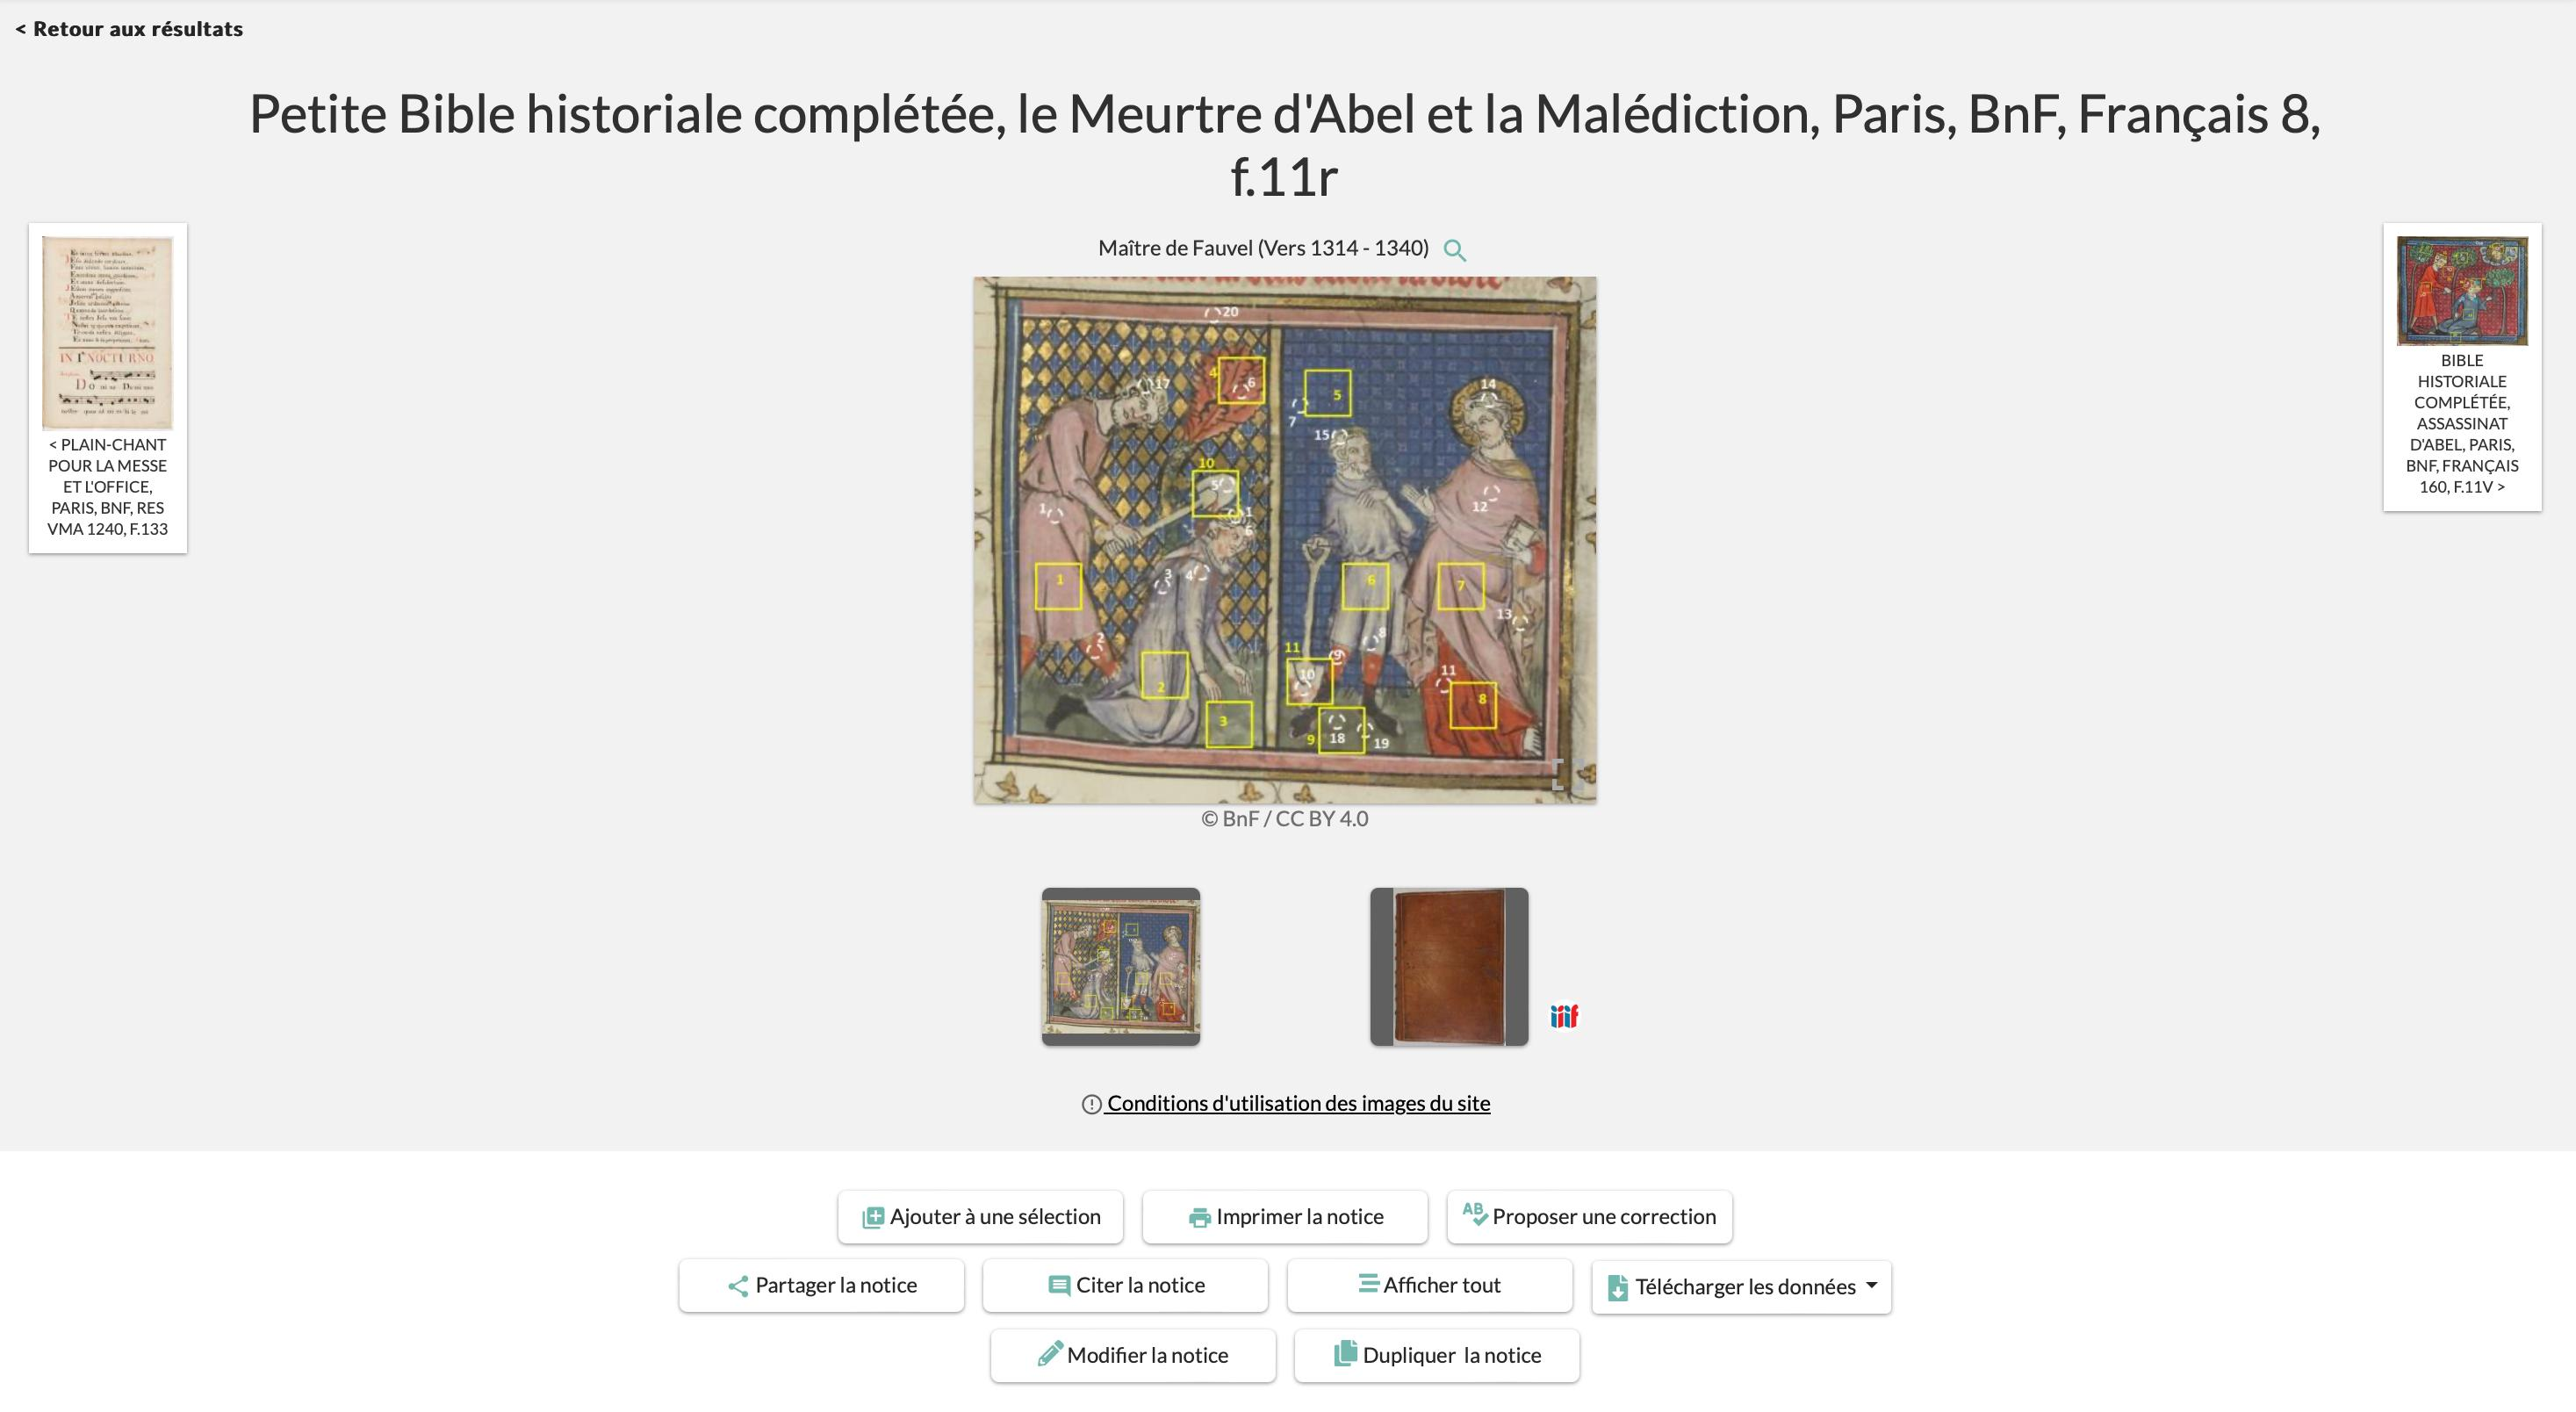
\includegraphics[width=\textwidth]{./textes/chap1/agorha-carrousel.jpg}
	\caption{Le média d'une notice Aghora}
	\label{fig:carrousel}
\end{figure}

Ensuite, la notice repose sur des champs de données structurées. Les informations sur les feuillets des manuscrits sont divisées entre plusieurs catégories, selon le besoin des projets. Pour le projet sur la couleur, huit champs de données sont retenus : l’identification, la localisation, la description (avec les analyses), la création, la qualification entre l’imprimé et le manuscrit, les liens entre les œuvres, la documentation et, pour finir, la gestion de la notice. Ces champs sont à leur tour divisés en de nouveaux qui contiennent les résultats des projets de recherche, soit sous la forme d’une entrée de \indexmot{thésaurus}, soit d’un texte libre entré par la personne qui saisit. \textit{Voir la figure~2.}\par

\begin{figure}[p]
	\centering
	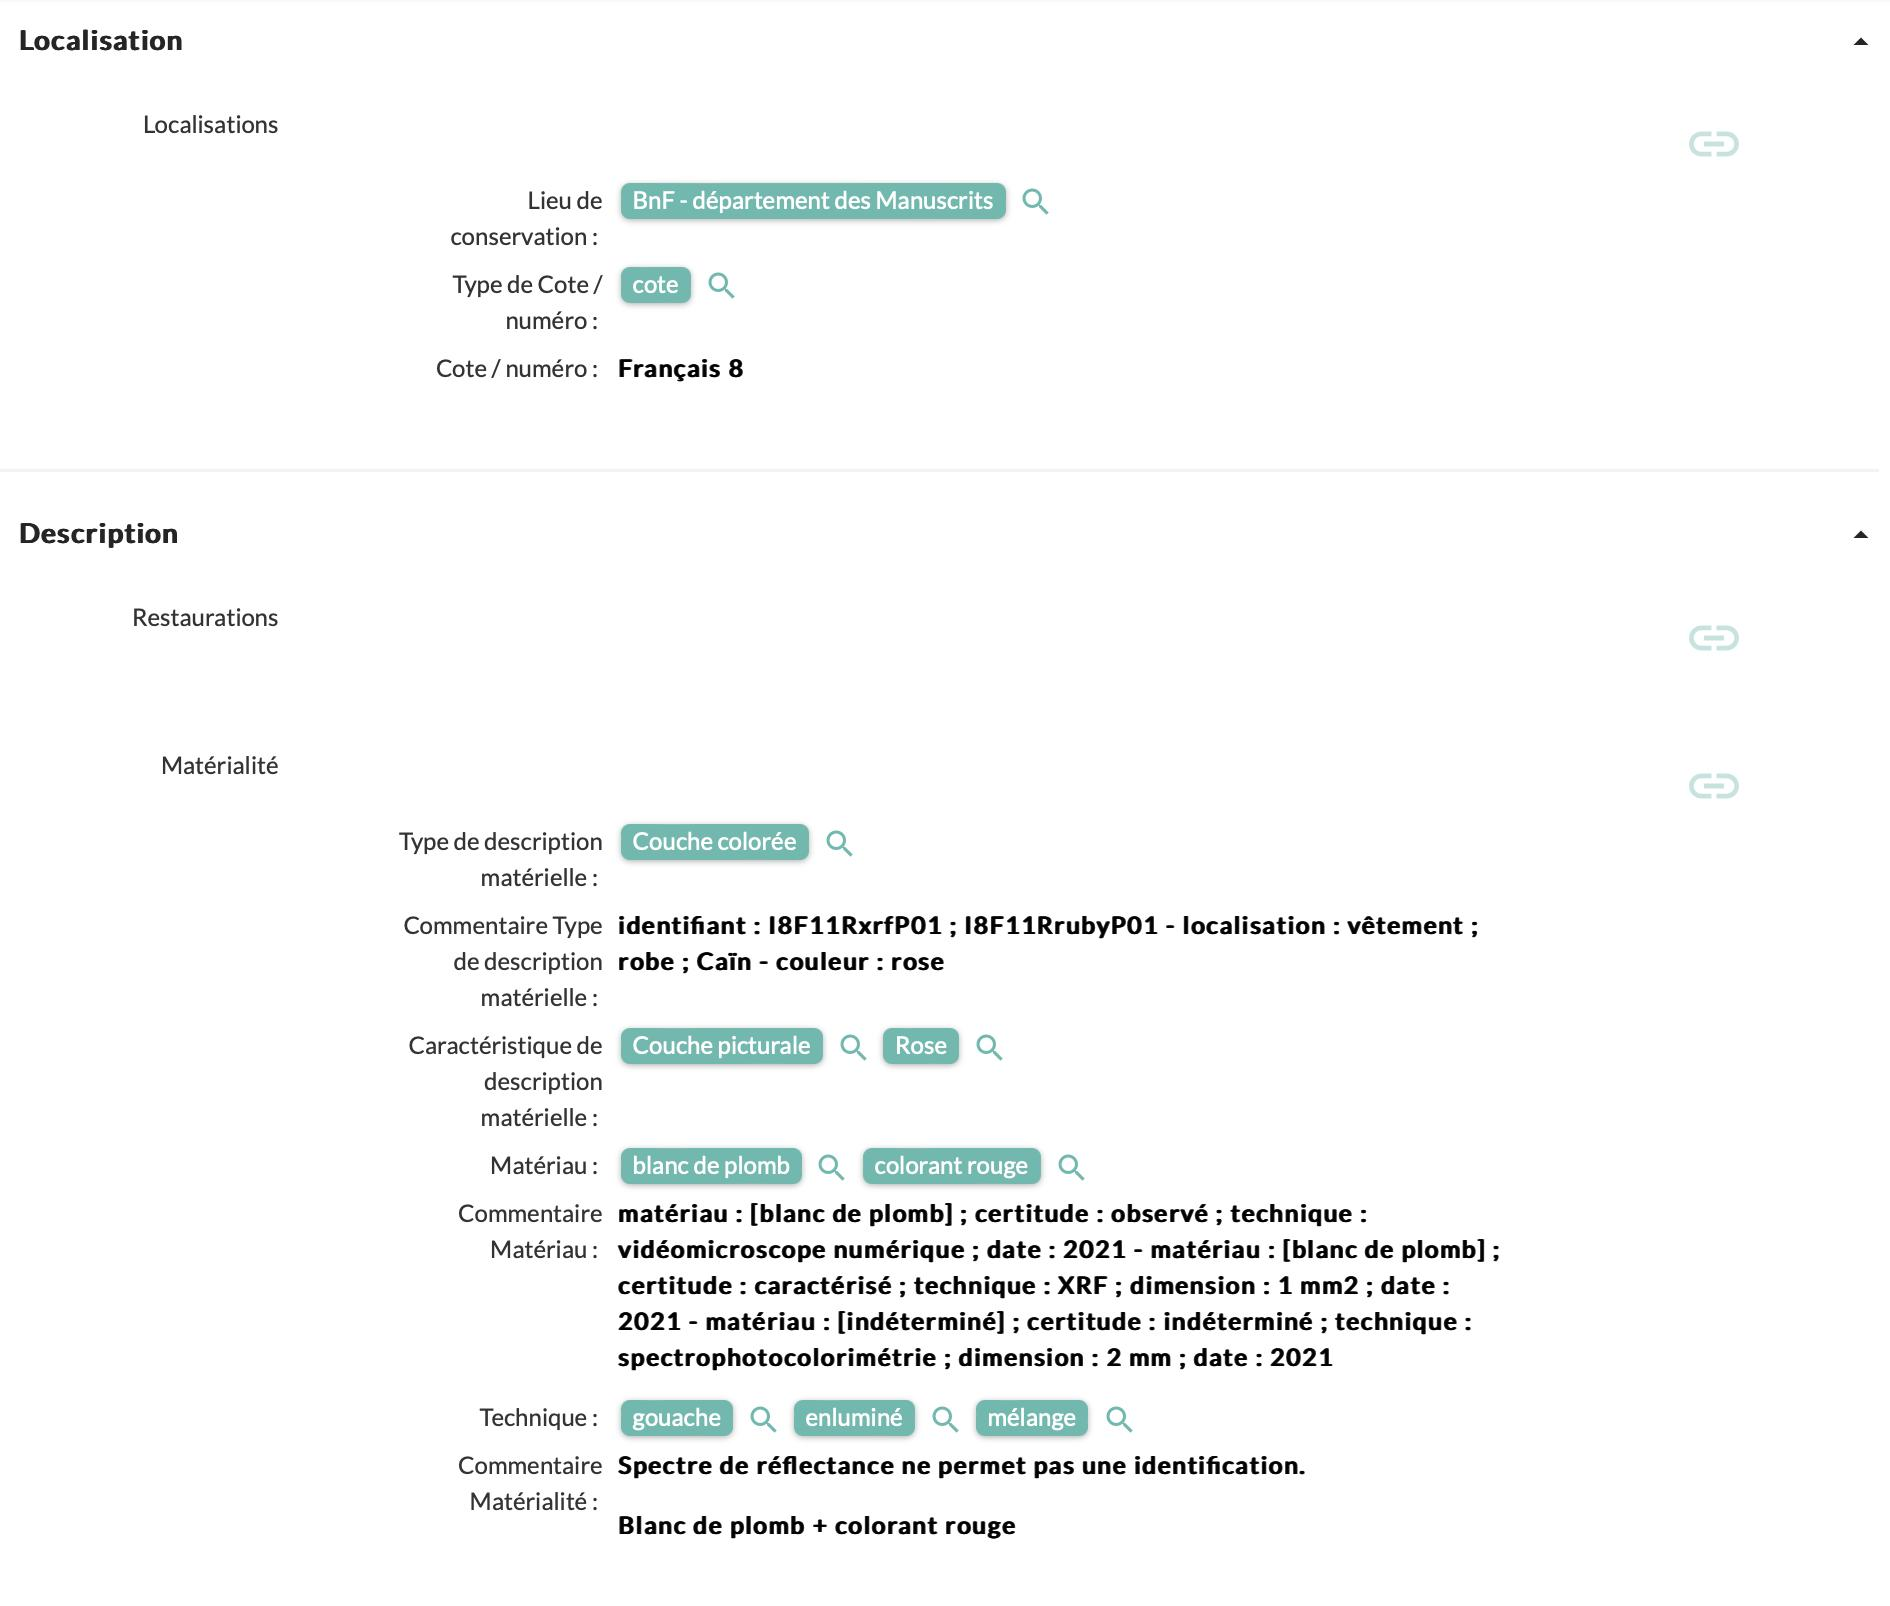
\includegraphics[width=\textwidth]{./textes/chap1/agorha-info.jpg}
	\caption{Les champs structurés sur Agorha}
	\label{fig:info}
\end{figure}

Les notices ont des identifiants uniques attribués automatiquement par le système informatique d’Agorha. L’identifiant est présent dans l’URL, c’est un UUID (Universally unique identifier). Pour retrouver une notice, il suffit ainsi de le renseigner à la fin de l’adresse d’Agorha~: \par
https://agorha.inha.fr/ark:/54721/ + UUID \\\par
En anticipant un peu sur la suite de ce mémoire, il convient ici de souligner que les notices œuvres concernent des feuillets de manuscrit. À titre d’exemple, le verso du feuillet~91 du manuscrit syriaque~47 a pour adresse https://agorha.inha.fr/ark:/54721/4308c58d-6569-489e-8d7d-a7436872b5cd?database=89. Son identifiant est donc~: 4308c58d-6569-489e-8d7d-a7436872b5cd. Ce système d’identification unique, avec le même nombre de caractères, facilite la récupération d’informations et la structuration des différentes notices entre elles, nous le verrons plus en avant. \par
Pour revenir à Agorha, ces identifiants uniformes permettent à la plateforme de s’insérer pleinement dans le web de données liées\footcite{pochon_agorha_nodate}. Ce dernier repose sur un ensemble de bonnes pratiques pour publier et relier des données structurées sur le web. Il vise principalement à faciliter l'intégration et l'interconnexion de données provenant de diverses sources. Agorha suit le modèle RDF (Resource Description Framework) qui représente les informations sous forme de triplet : un sujet, un prédicat, un objet. Par exemple, un feuillet (sujet) est réalisé à (prédicat) tel endroit (objet). La multiplication de triplets RDF permet de constituer un ensemble qui structure et interconnecte les informations. Les données liées peuvent ensuite être sérialisées avec du JSON-LD. Cette syntaxe permet de représenter des graphes RDF de manière compacte et facile à intégrer dans des applications web, tout en conservant les capacités de lien et de description du RDF. Dans Agorha, toutes les notices reposent sur du JSON-LD. Pour faire apparaître la méthode, il suffit de compléter les adresses de cette façon~:\par https://agorha.inha.fr/ark:/54721/ + UUID + .json. \newline\par
Si nous nous penchons sur le cas du manuscrit syriaque précédent, sa localisation apparaît ainsi en JSON-LD~:

\begin{lstlisting}[language=json]
"localizationInformation" : {
	"localization" : [ {
		"place" : {
			"thesaurus" : {
				"ref" : "https://thesaurus.inha.fr/thesaurus/resource/ark:/54721/bd1b5af3-9b44-49e9-98b8-b97ca10dd7f2",
				"prefLabels" : [ {
					"value" : "\indexmot{Bibliothèque nationale de France} (Paris)",
					"language" : "fre"
				} ],
				"conceptPath" : "/Europe/France/Ile-de-France/Paris/\indexmot{Bibliothèque nationale de France} (Paris)",
				"geoPoint" : "48.834355,2.373378"
			}
		},
		"institutionIdentifierType" : {
			"thesaurus" : {
				"ref" : "https://thesaurus.inha.fr/thesaurus/resource/ark:/54721/feccfc54-f2da-458a-a42c-530037a5132b",
				"prefLabels" : [ {
					"value" : "cote",
					"language" : "fre"
				} ],
				"conceptPath" : "/cote"
			}
		},
		"institutionIdentifier" : {
			"value" : "Syriaque 47",
			"language" : "fre"
		},
		"sourcing" : [ {
			"database" : {
				"ref" : "89",
				"value" : "La fabrique de l'art. Couleurs et matériaux de l'enluminure"
			}
		} ]
	} ]
}
\end{lstlisting} \par
Agorha permet donc une intégration structurée et interconnectée des résultats des deux programmes de recherche sur le web. La plateforme de l’INHA contribue à la science ouverte et la communication des résultats des analyses sur les enluminures et les panneaux peints selon les principes du web de données liées. \newpage

\section{Deux sites Omeka~S}

Les deux projets ne seront pas seulement présents sur la plateforme Agorha. L’INHA développe en ce moment deux sites Omeka~S qui permettront d’héberger, à partir de l’automne, les bases de données ainsi que les \indexmot{visualisation}s réalisées. Cette plateforme open source est spécifiquement conçue pour gérer des collections numériques dans l’optique d’une publication en ligne\footcite{noauthor_omeka_nodate}. Elle semble parfaitement correspondre aux attentes d’un projet de recherche scientifique comme ceux sur les manuscrits ou les panneaux peints.\par
En premier lieu, le site Omeka~S permet de créer des collections numériques. Ces dernières peuvent contenir les différentes notices présentes sur Agorha, mais avec une organisation et un archivage qui sont facilités. De plus, l’utilisation du schéma de métadonnées Dublin Core permet de reprendre les éléments des descriptions détaillées des notices. Il n’y a pas de perte de l’information et la normalisation reste. Ensuite, Omeka~S est conçu pour intégrer les données RDF que j’ai présentées précédemment. L’interconnexion entre les différentes données des résultats existera toujours. Il en est de même avec le JSON-LD. Omeka~S permet aussi d'accéder et de manipuler les données via des API, ce qui correspond aussi au critère d’interopérabilité voulu. Le principal avantage, au regard de la plateforme Agorha, réside dans la possibilité de le personnaliser pour les besoins spécifiques du projet. Le site public peut être structuré pour correspondre le mieux possible aux deux bases : navigation entre les onglets, liens entre les pages, visibilité des résultats ou encore insertion des \indexmot{visualisation}s. Le module de recherche lui-même peut être amélioré, afin d’orienter l’utilisateur vers des filtrages, option indispensable pour les projets scientifiques aussi complexes. Avec le site Omeka~S, les utilisateurs pourront sélectionner des paramètres parfois très précis pour isoler certains résultats ou croiser plusieurs filtres afin de faire apparaître des correspondances. En dernier lieu, un site conçu sur Omeka~S est traditionnellement conforme aux standards archivistiques et de gestion des collections, garantissant la pérennité des données. En outre, sa conception est conforme aux normes d’accessibilité, rendant le site utilisable par toute sorte de public.\par
En ce qui concerne les trois \indexmot{visualisation}s proposées pour les projets de recherche, leur intégration dans Omeka~S varie. L’intégration par iframe semble être la meilleure solution pour ce qui est de la \indexmot{carte interactive} et de la \indexmot{frise chronologique}. Un iframe, c’est~:\par
\begin{quote}
	« un élément HTML qui permet d'intégrer un contenu externe dans une page web. L'Iframe peut contenir une vidéo, une carte, une publication de réseau social ou encore une page web tierce. Le contenu s'affiche dans un cadre dont les propriétés peuvent être paramétrées à l'aide d'attributs.\footcite{thach_quest-ce_nodate} »
\end{quote}\par
En récupérant le contenu des deux \indexmot{visualisation}s et en personnalisant leur affichage, le site Omeka~S devrait permettre une navigation confortable pour l’utilisateur. Pour ce qui est des manifestes \indexmot{IIIF} et de leur exploration dans une visionneuse, il ne pouvait être raisonnablement proposé de passer par la solution d’un Iframe. En effet, Omeka~S permet d’implémenter directement une visionneuse, comme Mirador, dans le site réalisé. Cependant, la visionneuse étant insérée par un module propre à Omeka, elle ne possède pas les mêmes propriétés que celle en libre accès sur internet. Un problème de compatibilité des manifestes \indexmot{IIIF} est apparu alors, j’y reviendrai plus un avant.\newpage

\section{L’enjeu du \indexmot{thésaurus}}

Les \indexmot{visualisation}s sont, dans le fond, une certaine forme d’éditorialisation de la donnée. Elles reposent sur une interrogation des jeux et des entrées présents dans la base. Ainsi, plus les termes et les catégories utilisés lors de sa conception sont précis et cohérents, plus la \indexmot{visualisation} sera pertinente d’un point de vue scientifique au moment de sa réalisation. Il me semble que la constitution des \indexmot{thésaurus} a joué un rôle déterminant dans la réussite des deux projets et a permis d’envisager les différentes \indexmot{visualisation}s. Je souhaite donc m’y attarder un moment pour finir ce chapitre introductif. \par
Un \indexmot{thésaurus} est, en quelque sorte, une standardisation du vocabulaire. Son rôle est de garantir que les termes sont utilisés de manière uniforme tout au long du travail de recherche. C’est un vocabulaire contrôlé, qui doit prévenir les éventuelles ambiguïtés et incohérences dans le remplissage des données dans la base. Mais au-delà de cette normalisation, l’instauration d’un \indexmot{thésaurus} est fondamentale en ce qu’il contraint les chercheurs à une réflexion sur les termes utilisés et leur articulation les uns avec les autres. Ainsi, le \indexmot{thésaurus} aide à structurer la description. L’attribution d’un terme à une donnée, à une idée, à une réalité – ce qui est donc une indexation – peut induire une hiérarchie en fonction du vocabulaire retenu. Les données sont alors regroupées selon leur similarité et classées par une logique définie en amont. Ce vocabulaire nécessite un effort théorique de la part des coordinateurs du projet~: les termes doivent être justifiés et explicités et, bien souvent, une documentation est produite pour accompagner un \indexmot{thésaurus}. Elle permet de fournir des définitions claires et précises des termes, des orientations aussi quant à l’indexation à choisir. \\\par
Les porteurs du projet ne cachent pas que l’un des principaux défis a bien été la constitution d’un référentiel d’autorité sur les matériaux et les couleurs qui puisse être applicable à des techniques, des époques et des aires géographiques très diverses\footnote{Appel à projet « La couleur~: artefacts, matière et cognition »}. S’il existait déjà un \indexmot{thésaurus} de référence pour les sciences de la conservation\footnote{Vocabulaire contrôlé réalisé pour les projet PARCOURS, puis SOCORÉ.}, ce n’était pas le cas pour la couleur et ses composants. Quelques précédents étrangers peuvent servir d’exemples cependant, comme la base américaine CAMEO\footcite{conservation__art_materials_encyclopedia_online_pigment_nodate}. L’élaboration du référentiel des matières colorantes est un parfait exemple de la synergie entre les différentes traditions scientifiques qui entourent le projet, puisqu’elle est le fruit d’ateliers réunissant des spécialistes de diverses disciplines (historiens de l’art, chimistes, spécialistes des textes anciens, naturalistes, anthropologues, etc.) et des professionnels issus des institutions partenaires. 
Une fois créés, les \indexmot{thésaurus} « matériaux » et « techniques » viennent enrichir GINCO (Gestion d’Informations Communes). GINCO donne accès à l’ensemble des vocabulaires scientifiques et techniques produits par le Ministère de la Culture et ses partenaires\footcite[En 2024, le logiciel n’est plus maintenu à jour et semble voué à disparaître.]{ministere_charge_de_la_culture_culturecommunicationginco_2022}. L’INHA, pour ses projets, se fournit et alimente les vocabulaires établis, au  moyen du langage de requête SPARQL\footcite{inha_thesaurus_nodate}. De façon concrète, dans le cadre des deux projets qui nous intéressent, le chercheur qui saisit des données dans la base le fait par l’intermédiaire de champs de recherche. À ce moment, un petit moteur de recherche suggère par auto-complétion les termes qui pourraient convenir et qui sont présents dans GINCO. Si aucun terme ne convient, il faut que le chercheur demande son ajout dans le \indexmot{thésaurus}, le vocabulaire serait alors renseigné au format SKOS\footcite[« SKOS (Simple Knowledge Organisation System ou Système simple d’organisation des connaissances) est un langage de représentation de schémas de concepts, ce qui recouvre les langages documentaires tels que les \indexmot{thésaurus}, classifications, listes de vedettes matière, taxonomies, folksonomies, etc. Son nom a été choisi pour mettre en évidence l’objectif même visé par ce langage : proposer un système permettant d’exprimer et de gérer des modèles interprétables par les machines dans la perspective du web sémantique », ][]{lenart_skos_2007} pour pouvoir intégrer GINCO. Cette méthode de travail et de complétion de la base permet de s’assurer de la cohérence du vocabulaire utilisé et de sa normalisation.

Concernant les \indexmot{visualisation}s des jeux de données, la constitution d’un \indexmot{thésaurus} commun aux deux projets permet de les réunir au sein d’un même travail d’éditorialisation. L’utilisation d’un vocabulaire contrôlé identique, pour la recherche sur \enquote{La couleur~: artefacts, matière et cognition} et sur \enquote{La fabrique matérielle du visuel~: panneaux peints en Méditerranée}, autorise leur interrogation selon les mêmes critères et pour l’ensemble des résultats. Cette démarche simplifie aussi le travail technique qui poursuit les projets. La définition des filtres, qui sont les pivots de l’éditorialisation, ne représente dès lors plus un enjeu puisqu’ils sont communs et choisis par les chercheurs. Il n’y aura ni ambiguïté, ni incohérence. \newpage

* \\

Depuis le début du projet, en janvier 2021, les différents porteurs ont œuvré pour que les données constituées dans la base s’inscrivent dans les nouvelles recommandations de l’interopérabilité et dans une politique de science ouverte. La communication des résultats avec le public des chercheurs est pensée en deux temps~: une première sur la plateforme Agorha de l’INHA, où les données rejoignent~–~et sont valorisées avec~–~d’autres programmes de recherche en histoire de l’art et archéologie~; et une seconde, avec une migration des données vers deux sites Omeka~S, afin d’individualiser et de personnaliser les résultats du projet. La constitution de \indexmot{thésaurus} identiques aux deux recherches permet de proposer des \indexmot{visualisation}s communes et ainsi de poursuivre leur collaboration.
	
	\chapter{Ordonner les données dans l'espace, la carte interactive}
	Le projet \enquote{La couleur~: artefacts, matière et cognition} repose sur plus de 8~000 analyses. Ces dernières se déclinent en une multitude d’informations, de définitions et de commentaires qui sont, en les situant dans un contexte informatique, autant de variables pour un traitement personnalisé de la recherche. Dans le cadre d’une politique d’éditorialisation des données par les utilisateurs, il me semble que proposer la mise en ordre des données dans l’espace est l’une des plus importantes. Les chercheurs ont réuni, au cours des années du projet, des informations précieuses sur les lieux de création des œuvres. Illisibles dans l’immensité d’un fichier~CSV, la représentation de ces données sur une carte permet de produire une distribution dans l’espace de la production artistique et, ainsi, de faciliter l’interprétation avec une approche géographique.\newpage

\section{\indexmot{Leaflet}~: une bibliothèque JavaScript open-source et légère}

La cartographie interactive est un outil précieux pour visualiser et interagir avec des données géographiques de manière dynamique et intuitive. \par
Les données de la base des projets de recherche sont une véritable mine d’informations. Elles n’auraient pu que s’appauvrir en les représentant avec une carte statique classique. Premièrement, cette dernière est contrainte par une image numérique qui prédéfinit une dimension et une résolution, là où la \indexmot{carte interactive} permet des manipulations d’échelles qui évitent les excessives accumulations de données. Ensuite, elle ne permet pas de représenter les variables temporelles, à moins d’être multipliées en autant d’exemplaires que de dates voulues. Enfin, la carte classique ne représente finalement qu’une \indexmot{visualisation} des informations conçue et produite par un cartographe, sans personnalisation possible par l’utilisateur. Sans lister exhaustivement toutes les contraintes – et les limites – d’une telle représentation, ces petits exemples permettent de mesurer la nécessité de réaliser dans le cas présent une cartographie interactive, plus  complexe, mais plus fidèle à la richesse des données de la base.\\\par
Aujourd’hui une \indexmot{carte interactive} peut être réalisée à l’aide d’outils et de plateformes en ligne, comme Google My Maps\footcite{noauthor_google_nodate}, Mapbox\footcite{noauthor_mapbox_nodate} ou encore ArcGIS Online\footcite{noauthor_arcgis_nodate}. Ces plateformes sont gratuites et accessibles à toute personne possédant des rudiments d’informatique, mais elles ne parviennent pas à offrir autant d’avantages et de fonctionnalités que les outils qui nécessitent des connaissances en codage. Ces derniers permettent de personnaliser presque toutes les options de la carte, y compris l’apparence, le comportement et les fonctionnalités. Ils sont réputés avoir une meilleure performance si le nombre de données est amené à être important et, surtout, les outils reposant sur du codage peuvent être plus facilement intégrés dans des applications ou sites Web – comme il en est dans le cas présent. 
Les outils de cartographie sont, pour l’essentiel, des bibliothèques JavaScript, en raison de la simplicité, de l’interactivité et de la performance de ce langage. Il possède également une grande communauté de développeurs qui contribuent à le maintenir à jour et à proposer toujours de nouvelles solutions aux utilisateurs. La communauté JavaScript a développé quelques outils populaires, comme \indexmot{Leaflet}.js\footcite{agafonkin_leaflet_nodate}, OpenLayers\footcite{noauthor_openlayers_nodate}, D3.js\footcite{noauthor_d3_nodate} ou encore Mapbox GL JS. Dans le cadre de ce stage, le choix de la bibliothèque \indexmot{Leaflet}.js, bien qu’elle soit réputée comme étant la plus légère, est apparu comme une évidence. Elle propose, malgré sa simplicité, une large gamme de fonctionnalités de cartographie, notamment en ce qui concerne les marqueurs, les pop-ups, la possibilité de cumuler les filtres ou encore de faire apparaître une barre latérale. Elle propose déjà, en somme, toutes les options qui ont été retenues pour la \indexmot{visualisation} interactive\footnote{Cf. infra.}. De plus, elle est utilisée couramment par le service informatique de l’INHA, service qui hébergera la base Omeka~S du projet\footnote{À titre personnel, la bibliothèque \indexmot{Leaflet} est aussi celle qui me fut enseignée au cours de cette année de master.}. Dans le cadre d’un stage d’une durée de trois mois et avec les conditions énoncées préalablement, il ne m’a pas semblé opportun de continuer l’investigation vers les autres bibliothèques, mais au contraire plus pertinent de chercher à déployer pleinement toutes les potentialités de la bibliothèque \indexmot{Leaflet}. Ainsi, les fonctionnalités plus avancées d’OpenLayers, notamment quant aux tuiles ou aux images raster n’étaient d’aucun intérêt dans le cas présent, D3.js n’est pas nativement conçu pour de la cartographie et aurait complexifié inutilement le travail, tandis que la dernière bibliothèque, Mapbox GL JS, semble plus convenir à un autre public que celui de chercheurs au regard de l’éditorialisation à venir.\\\par
À la date du 18 mai 2023, \indexmot{Leaflet} est à sa version 1.9.4\footnote{Pour notre part, nous avons réalisé le travail à partir de la version 1.8.0.}. La bibliothèque est déposée et peut-être librement téléchargée sur la plateforme GitHub~–~elle pèse seulement 42~ko de JS. Son premier développeur, l’Ukrainien Vladimir Agafonkin, s’est entouré depuis une dizaine d’années d’une petite équipe qui veille au maintien de \indexmot{Leaflet}. La bibliothèque répond ainsi aux innovations du web et aux nouveaux besoins des utilisateurs. Pour ces derniers, les développeurs déposent à l’adresse https://leafletjs.com des tutoriels et une riche documentation qui apportent une réponse à la plupart des questions et des difficultés rencontrées.\par
Une fois téléchargé, le code se divise en trois fichiers et un dossier\footcite{agafonkin_leaflet_nodate}~: 
\begin{itemize}
	\item \texttt{leaflet.js}~: il s’agit du code minifié\footnote{En programmation, minifier signifie réduire la taille du code.}
	\item \texttt{leaflet-src.js}~: le code non-minifié cette fois-ci, ce qui peut permettre un débogage
	\item \texttt{leaflet.css}~: la feuille de style
	\item \texttt{images}~: un dossier contenant les images référencées par le fichier précédent\\
\end{itemize}

Cet ensemble doit être décompressé et placé dans le répertoire du site web. Sur la page HTML, il suffit d’ajouter ces deux lignes pour créer le lien avec la bibliothèque \indexmot{Leaflet}~:\par
<link rel="stylesheet" href="/chemin/vers/le/fichier/leaflet.css" />\par
<script src="/chemin/vers/le/fichier/leaflet.js"></script> \\\par

Les fichiers JavaScript sont alors correctement liés à la page~HTML qui permet de visualiser et déployer la carte sur le site web. Avant de débuter le traitement de la donnée, il convient de poursuivre le travail préparatoire sur les objectifs de la \indexmot{visualisation} et de définir, avec une plus grande précision, les attendus de l’éditorialisation.\newpage

\section{Éditorialiser une base de données avec une cartographie interactive}

La constitution de la base de données par les chercheurs du projet, notamment à partir des \indexmot{thésaurus}, permet d’avoir à disposition des variables qui seront à l’origine de l’éditorialisation. Concrètement, il s’agit dans le cadre d’une cartographie interactive de réaliser le choix d’un ou de plusieurs filtres qui s’appuient sur des clefs, représentées par des colonnes dans les fichiers~CSV, et de porter la sélection sur les valeurs associées, limitées raisonnablement par le \indexmot{thésaurus}. À titre d’exemple, que ce soit pour la base materiality88 ou celle 89, au sein de la colonne \enquote{schema:color} qui représente les couleurs identifiées au moment de l’analyse, le filtre porte sur une sélection entre quinze valeurs~: argenté, beige, blanc, bleu, brun, cuivré, doré, gris, jaune, noir, orange, rose, rouge, vert et violet. Une attribution définie au moment de l’analyse scientifique de l’objet devient ainsi ici une variable qui permet d’éditorialiser~–~de filtrer~–~le résultat pour l’utilisateur.\par
La cartographie interactive est une \indexmot{visualisation} parfaitement adaptée à ce processus de sélection, de désélection et de combinaison de filtres. À la manière des cartes statiques qui laissent une place aux légendes, celles interactives permettent de faire apparaître au plus près les besoins en information et en usage pour l’utilisateur. Elles prennent la forme de quadrilatères équiangles pouvant être disposés selon les souhaits du cartographe. Dans notre cas présent, l’éditorialisation se réalise à partir de quatre filtres, qui peuvent tous s’additionner afin d’affiner la recherche.\\\par
La \indexmot{visualisation} a pour objectif de traduire la circulation et l’utilisation des matériaux de couleur dans la fabrique des enluminures et des panneaux peints sur plus d’un millénaire. C’est une \indexmot{visualisation} qui est non seulement géographique, mais également chronologique. Elle repose ainsi sur quatre variables présentes dans les bases de données~: le matériau (schema:material), la couleur obtenue (schema:color), la localisation (schema:geo) et la date de création (crm:P4\_has\_time-span). Toutes les autres informations présentes dans les bases servent à enrichir les informations proposées par les résultats du filtre, mais elles ne constituent pas les pivots de l’éditorialisation.\par
La première option à la disposition de l’utilisateur émane d’une demande des responsables du projet. Madame Charlotte Denoël, responsable du projet \enquote{La couleur~: artefacts, matière et cognition}, et madame Sigrid Mirabaud, responsable du programme \enquote{La fabrique matérielle du visuel}, souhaitent laisser le choix entre une navigation qui réunirait les deux projets et une autre, qui porterait exclusivement sur l’un d’entre eux. Si les deux projets sont réunis sur la plateforme Omeka~S en raison de leur synergie, ils doivent pouvoir être individualisés à la demande. Ainsi, il convient d’insérer un filtre qui permet la bascule d’un projet à l’autre en première option, tout en proposant leur réunion~–~choix initialisé par défaut.\par

\begin{figure}[H]
	\centering
    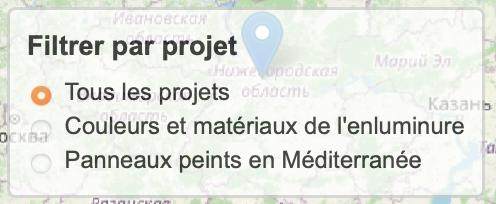
\includegraphics[scale=0.4]{./textes/chap2/filtre-projet.jpg}
	\caption{Filtrer par projet sur la carte}
	\label{fig:info}
\end{figure}

Afin de visualiser l’évolution dans le temps des données, le filtre sur les dates de création est sous la forme d’une jauge. Cette dernière, plus intuitive, est plus à même d’offrir une interaction fluide à l’utilisateur, qui n’a qu’à faire glisser le curseur pour sélectionner une année spécifique. Quant à la granularité de la jauge, les deux bases de données couvrant plus d’un millénaire, j’ai décidé de réaliser une sélection par décennie plutôt que par années. Ce choix doit rendre plus aisé les tendances sur la carte, par une apparition plus fréquente des données. De plus, ce filtre n’est pas, en quelque sorte, \enquote{excluant}, mais au contraire inclut et ajoute progressivement de la donnée à la carte~: le filtre ne représente pas seulement une décennie, mais additionne les créations de ces dernières à celles préexistantes. Ainsi, si nous déplaçons le curseur sur l’année 1060, les manuscrits créent au cours de la décennie s’ajouteront à ceux antérieurs, sans les remplacer. Il me semble que c’est ici proposer une vision plus globale d’un contexte de production, en ne l’isolant pas des dynamiques passées.\par

\begin{figure}[H]
	\centering
	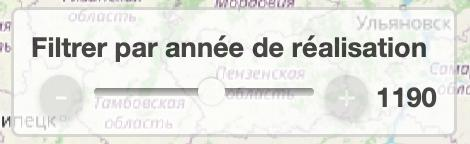
\includegraphics[scale=0.3]{./textes/chap2/filtre-annee.jpg}
	\caption{Filtrer par année sur la carte}
	\label{fig:info}
\end{figure}

La troisième variable est la plus importante du projet. Elle repose sur l’analyse des matériaux et sur leur ontologie. Que ce soit pour la base materiality88 ou celle 89, ces données sont entrées au sein de l’entité \enquote{schema:material}. Fruit d’un long travail, elles reflètent aussi la difficulté de la coordination et de la description manuelle sur un tel corpus. Un script Python révèle qu’à la date du 15~mai 2024, lors d’un travail de normalisation encore en cours, l’entité \enquote{schema:material} possédait 258~valeurs différentes, loin du \indexmot{thésaurus} constitué. Des erreurs d’écriture, plus que de choix, expliquent le résultat~–~nous le remarquons notamment par la présence d’apostrophes qui déprécie l’uniformité\footnote{On rencontre ainsi 1050 occurrences de \enquote{blanc de plomb}, 12 de \enquote{blanc de plomb’} et 10 de \enquote{‘blanc de plomb}.}. De ce fait, un filtre reposant sur une simple sélection n’est pas envisageable. Je propose, pour le choix du matériau, un champ de recherche avec de l’auto-complétion afin de guider l’utilisateur parmi toutes les valeurs~–~l’ordre de la valeur recherchée n’a pas d’importance et le filtre peut être nettoyé à tout moment.\par

\begin{figure}[H]
	\centering
	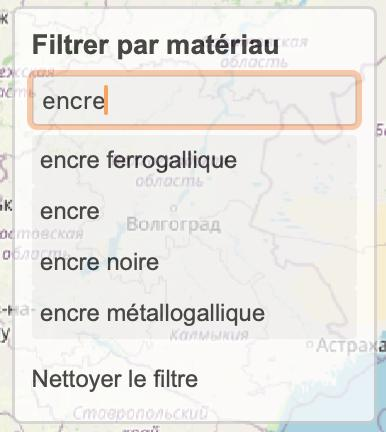
\includegraphics[scale=0.3]{./textes/chap2/filtre-materiaux.jpg}
	\caption{Filtrer par matériau sur la carte}
	\label{fig:info}
\end{figure}

Le dernier et quatrième filtre visible sur la carte porte sur les couleurs. Il semble utile de faire apparaître la concordance ou, au contraire, la discordance de cette variable avec la précédente. Le cumul de ces deux filtres fait ainsi apparaître un maintien ou une disparition de marqueurs que les chercheurs pourront interpréter. Cette entité ne reposant que sur quinze valeurs, j’ai opté pour un sélecteur à choix multiples.\par

\begin{figure}[H]
	\centering
	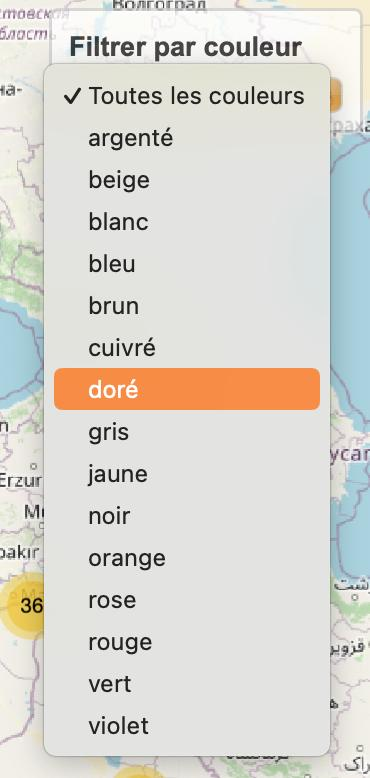
\includegraphics[scale=0.3]{./textes/chap2/filtre-couleur.jpg}
	\caption{Filtrer par couleur sur la carte}
	\label{fig:info}
\end{figure}


L’ensemble de la \indexmot{carte interactive} repose la présence de marqueurs, qui représentent la ou les localisations des feuillets analysés. Ces informations sont entrées au sein de l’entité \enquote{schema:geo}. Cette dernière contient des données de coordonnées géographiques, au format \enquote{latitude, longitude}. Un feuillet peut avoir plusieurs localisations possibles, dans le cadre de contexte de production pluriel ou indéterminé. Au lieu de choisir arbitrairement une seule coordonnée, un même feuillet peut apparaître sur la carte à plusieurs reprises~–~à la condition que les localisations soient éloignées d’au moins trois points de coordonnées pour ne pas surcharger inutilement la \indexmot{visualisation}. Ainsi, le \textit{Pentateuque dit d’Ashburnham ou de Tours} apparaît aussi bien en Afrique du nord, en Espagne, en Italie qu’en France\footnote{\textit{Pentateuque dit d’Ashburnham ou de Tours}, Paris, BnF, NAL 2334}. Lorsqu’ils sont en nombre, les marqueurs sont réunis en clusters – ils sont groupés. Ces derniers indiquent par un chiffre ou un nombre le total des feuillets qu’ils contiennent. Par un agrandissement de la carte ou un clic sur le repère, les marqueurs des feuillets apparaissent. Dans l’exemple ci-dessous, un clic sur le cluster vert situé au niveau de la ville de Milan fait apparaître quatre feuillets analysés du \textit{Liber comitis dit Lectionnaire pourpré}\footnote{\textit{Liber comitis dit Lectionnaire pourpré}, Paris, BnF, Latin 9451}.\par

\begin{figure}[H]
	\centering
	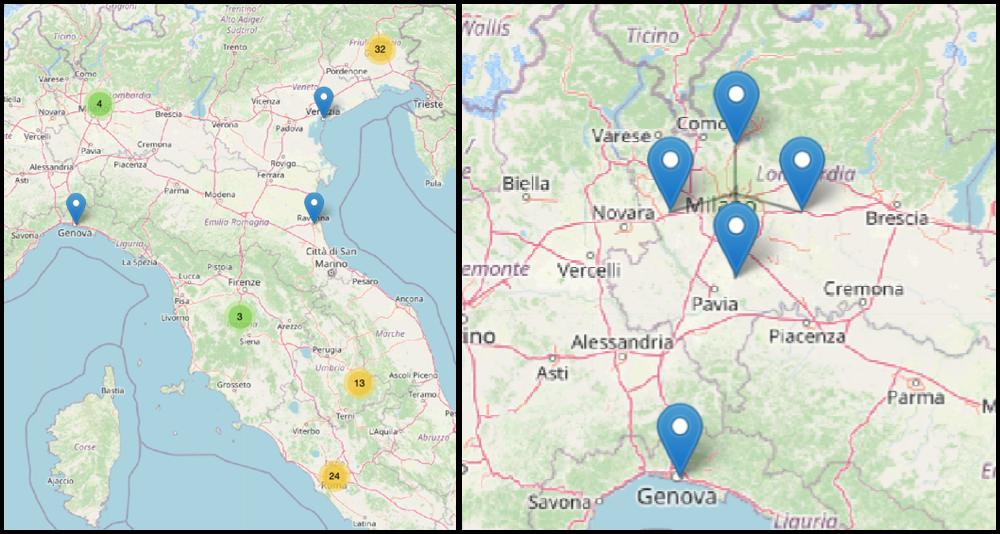
\includegraphics[scale=0.3]{./textes/chap2/localisation.jpg}
	\caption{Marqueurs et clusters}
	\label{fig:info}
\end{figure}

Il est apparu, dans le cadre du projet, qu’il est parfois impossible de proposer une localisation, même indécise, à un manuscrit. Dans ce cas de figure, je prends le parti de définir une localisation par l’absurde afin de faire figurer le marqueur. Situé au large des cotes bretonnes, dans l’Atlantique, le marqueur ne laisse pas de place à une ambiguïté. Une fois le carrousel déployé, il apparaît comme titre du feuillet l’indication \enquote{Lieu de création inconnu}.\\\par
À son lancement, la carte a, par défaut, tous les filtres ouverts et donc tous les marqueurs de représentés. Le filtre \enquote{projet} affiche les résultats sur les deux bases materiality, la date est dans sa dernière décennie, aucun matériau n’est sélectionné, ni aucune couleur définie. L’affichage est centré sur l’Europe et le bassin méditerranéen, où se situent les principaux manuscrits analysés – je crois en l’interactivité de la carte pour que l’utilisateur ait la curiosité de la décentrer et de découvrir des analyses sur des manuscrits produits en d’autres continents. \par

\begin{figure}[H]
	\centering
	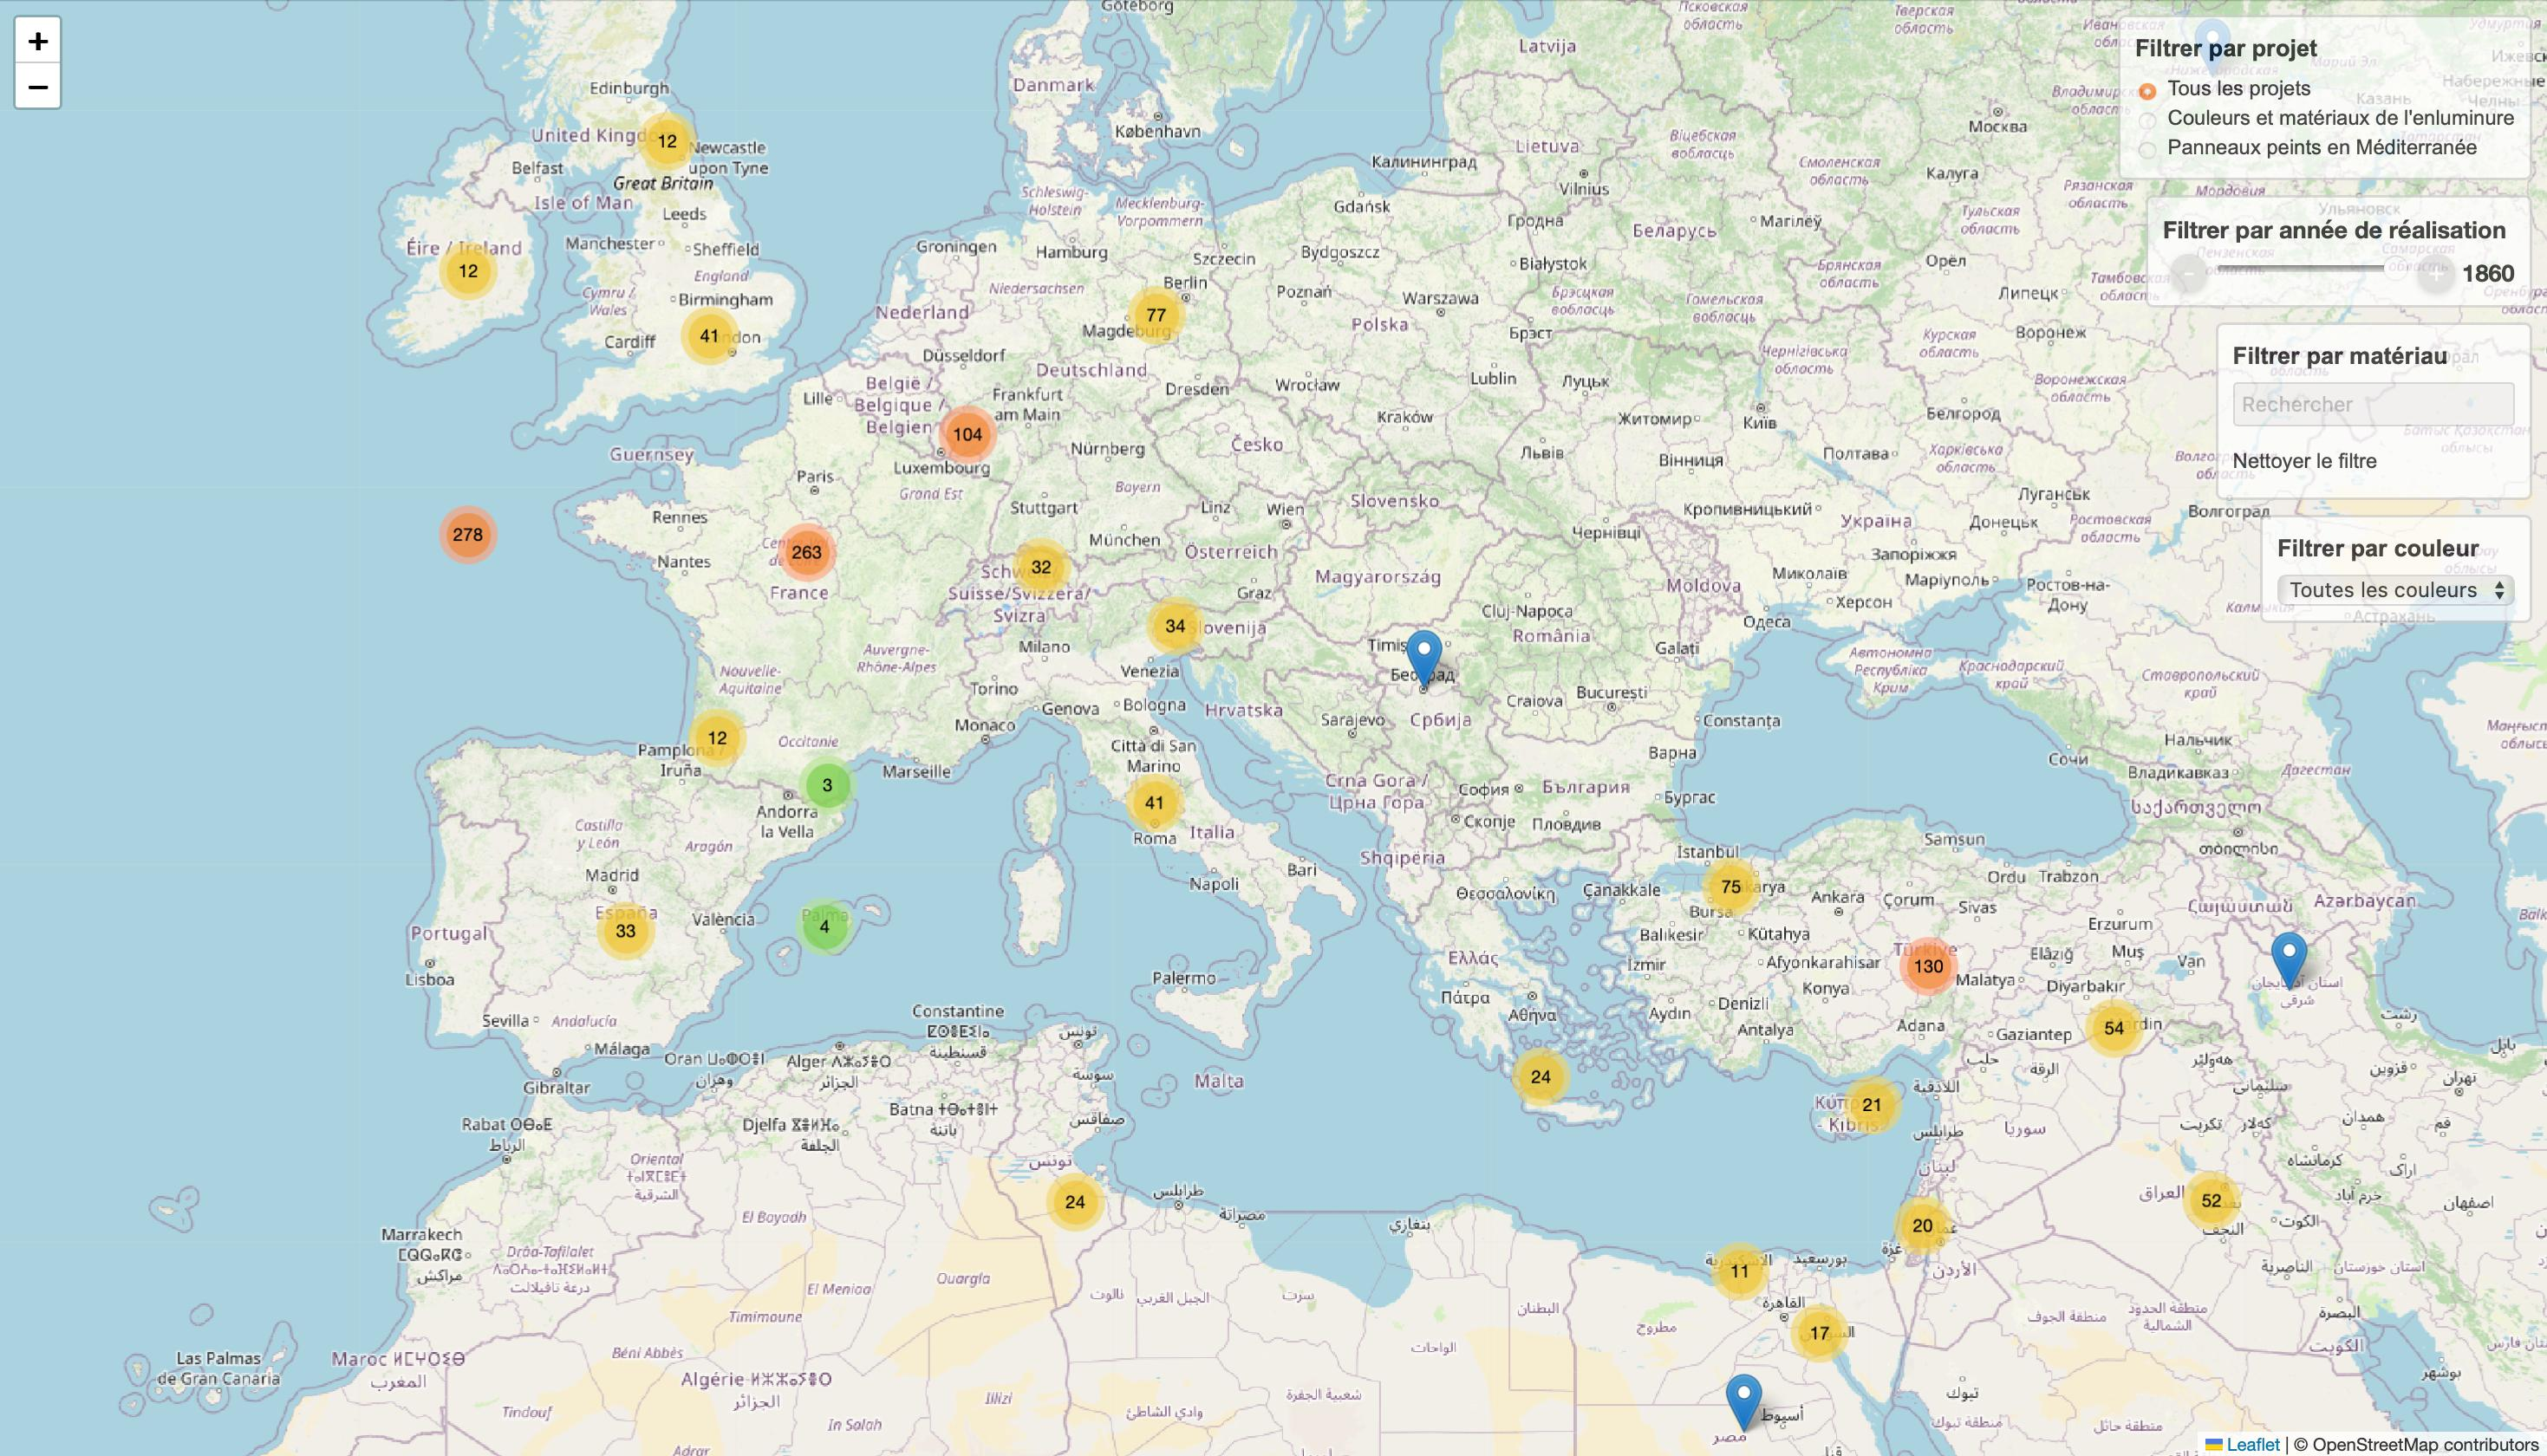
\includegraphics[width=\textwidth]{./textes/chap2/filtre-initialisation.jpg}
	\caption{Initialisation de la carte}
	\label{fig:info}
\end{figure}

Il a été loué précédemment la vertu heuristique du cumul des différents filtres~—~du croisement de variables en interrogeant la base~—~afin de faire apparaître certains résultats dans un contexte géographique et chronologique. La \indexmot{visualisation} ci-dessous, en quatre temps, est insérée à titre d’exemple afin d’apprécier l’efficacité de l’entonnoir produit par les filtres. En partant de la carte initialisée comme précédemment, je définis successivement une base de recherche, les \enquote{Couleurs et matériaux de l’enluminure}, un cadre chronologique avec l’année 1070, la cochenille pour matériau ainsi que la couleur rose. Il apparaît alors vingt-quatre résultats. \textit{Voir la figure 2.7.}\par

\begin{landscape}
	\begin{figure}[ht]
		\centering
		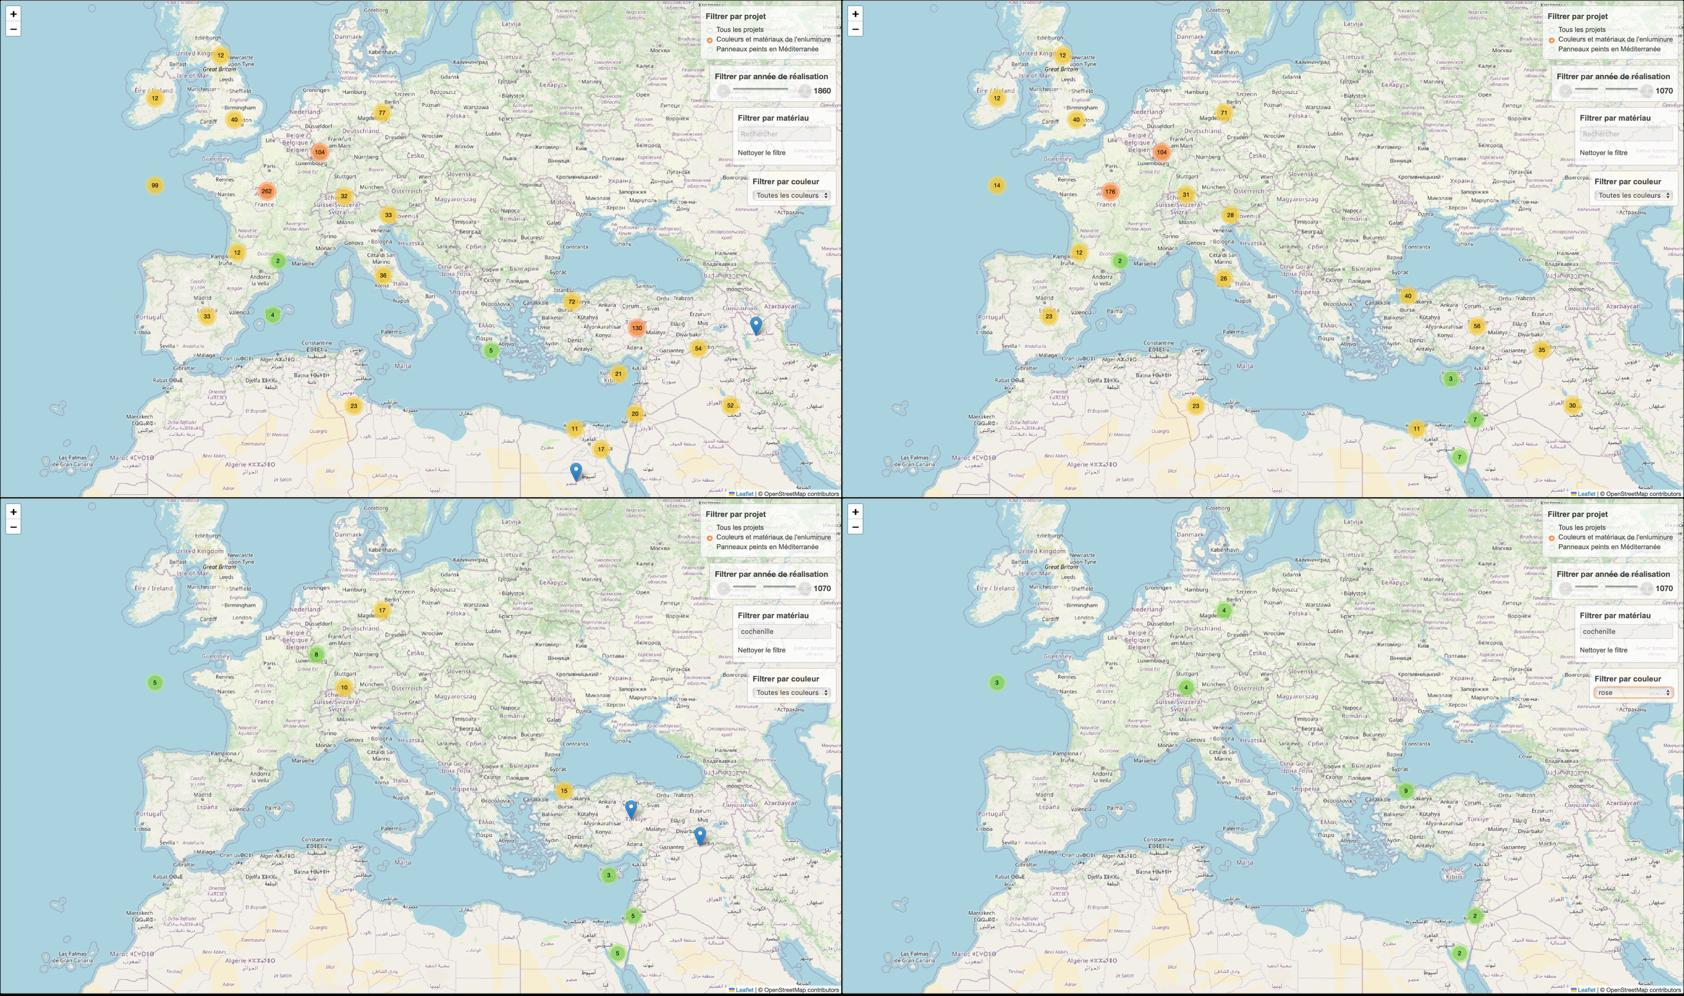
\includegraphics[scale=0.4]{./textes/chap2/filtre-4.jpg}
		\caption{Exemple d'éditorialisation}
		\label{fig:info}
	\end{figure}
\end{landscape}

La lecture des résultats est proposée en trois temps, qui représentent autant de niveaux de détails. Une première info-bulle apparaît lorsqu’un marqueur est survolé par le curseur. Elle reprend l’information entrée dans la colonne \enquote{dcterms:title} et informe sur le titre du manuscrit, sa cote, le nom du feuillet et son numéro. Ce survole rapide accélère le temps de recherche lorsque l’utilisateur est à la recherche d’un feuillet ou d’un manuscrit précis.\textit{Voir la figure 2.8.}\par

Ensuite, un clic permet de déployer un carrousel qui contient les données essentielles sur le feuillet~: une reprise de la colonne \enquote{dcterms:title} comme titre, suivie de l’appel à une image \indexmot{IIIF}~–~image qui peut être agrandie en haute résolution par un nouveau clic. Le carrousel permet une navigation entre les différentes analyses réalisées sur le feuillet. On y trouve ainsi la caractéristique, le motif, la technique, la couleur ainsi que le matériau. \textit{Voir les figures 2.9 et 2.10.}\par


\begin{landscape}
	\begin{figure}[p]
		\centering
		\centering
		\begin{minipage}{0.65\linewidth} % Trois images à gauche
			\centering
			\begin{minipage}{\linewidth}
				\centering
				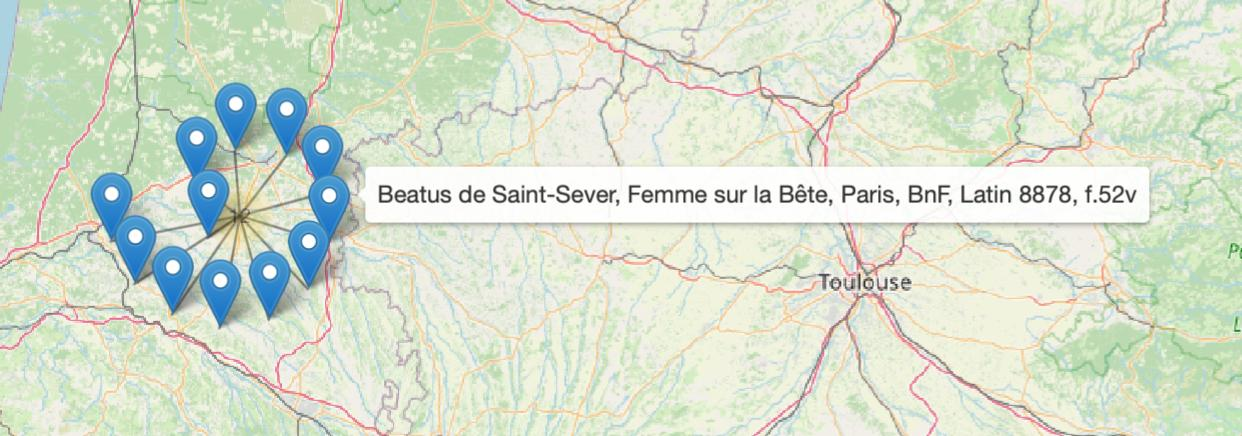
\includegraphics[scale=0.15]{./textes/chap2/info-bulle.jpg}
				\captionof{figure}{Une info-bulle avec les premières informations}
				\label{fig:info1}
			\end{minipage}
			\par\bigskip
			\begin{minipage}{\linewidth}
				\centering
				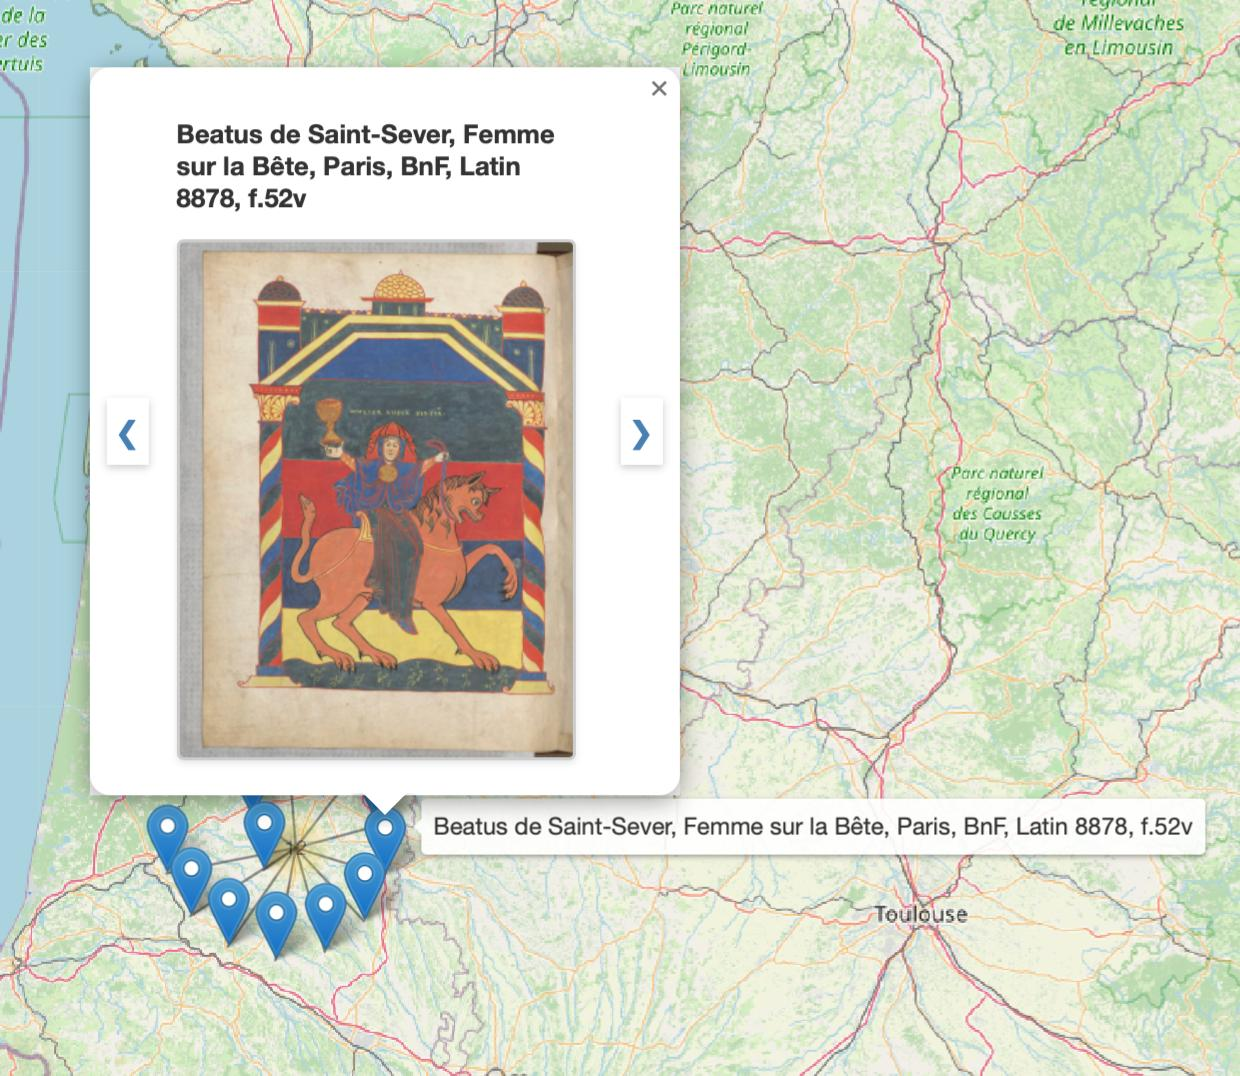
\includegraphics[scale=0.15]{./textes/chap2/carrousel-1.jpg}
				\captionof{figure}{Une image du carrousel}
				\label{fig:carrousel1}
			\end{minipage}
			\par\bigskip
			\begin{minipage}{\linewidth}
				\centering
				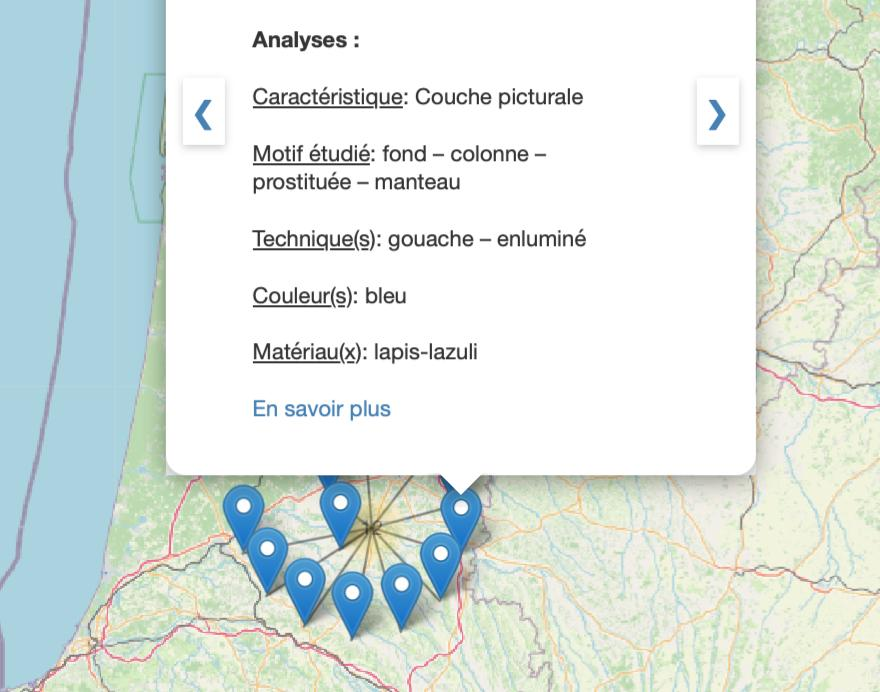
\includegraphics[scale=0.2]{./textes/chap2/carrousel-2.jpg}
				\captionof{figure}{Un descriptif du carrousel}
				\label{fig:carrousel2}
			\end{minipage}
		\end{minipage}\hfill
		\begin{minipage}{0.3\linewidth} % Une image à droite
			\centering
			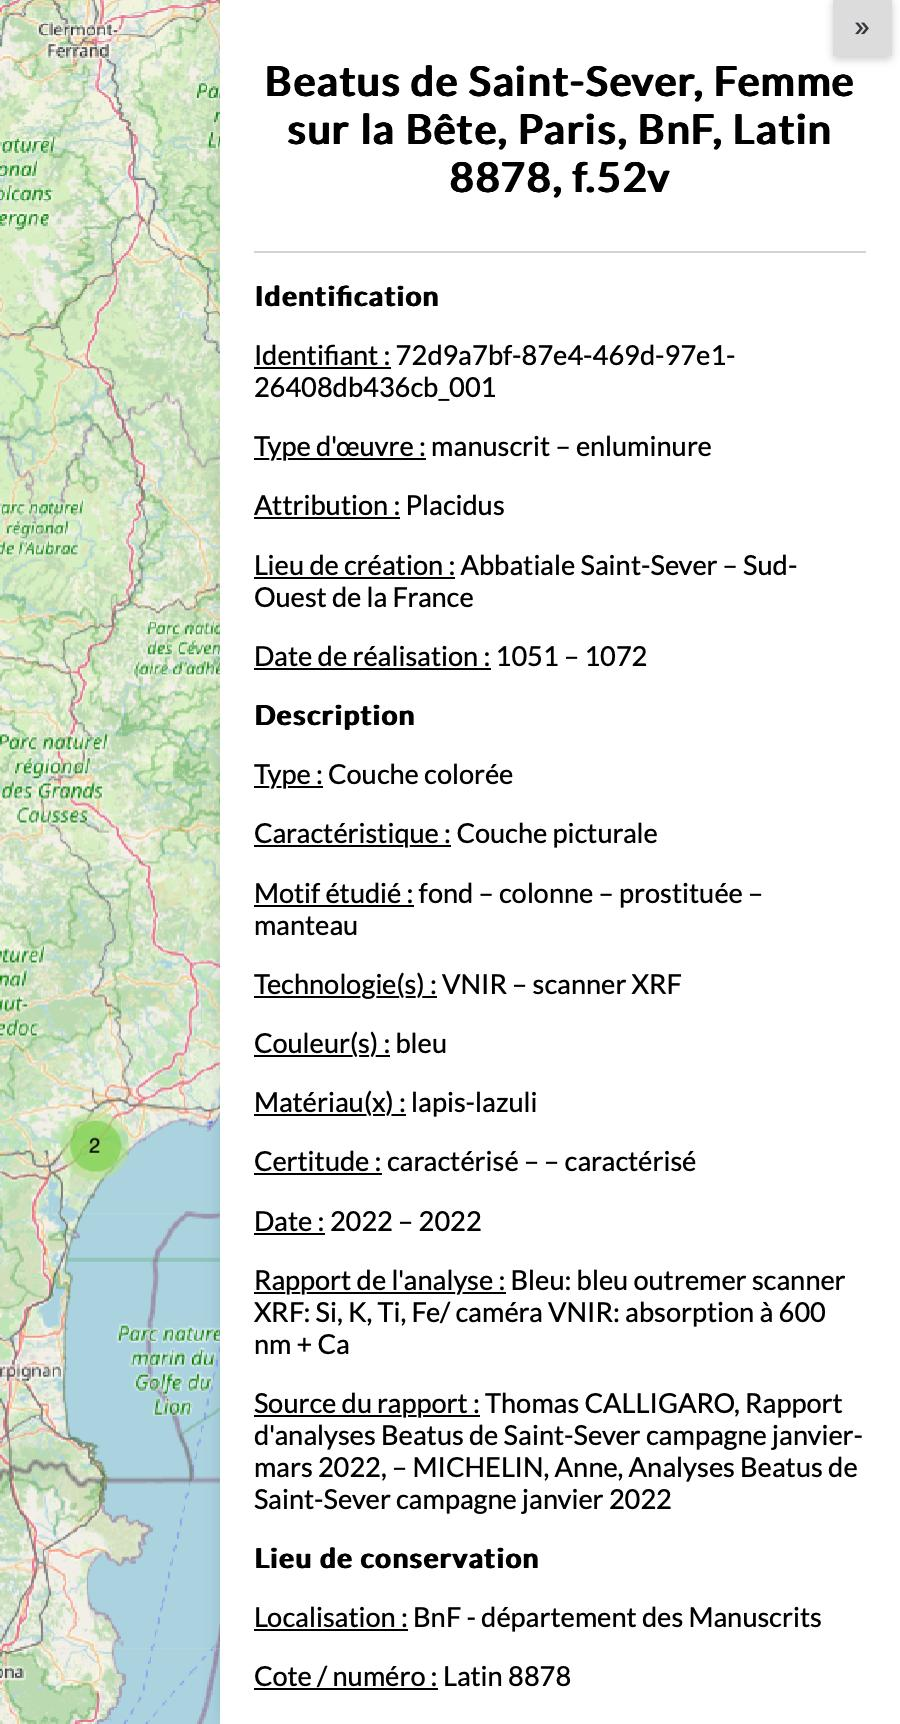
\includegraphics[scale=0.25]{./textes/chap2/slidebar.jpg}
			\caption{Une barre latérale avec la totalité des informations}
			\label{fig:info2}
		\end{minipage}
	\end{figure}
\end{landscape}

Lorsque l’utilisateur trouve le feuillet qui l’intéresse, il peut faire apparaître une barre latérale qui reprend et complète les informations présentes. Il apparaît alors le lieu de création, une éventuelle attribution, d’avantage de détails sur l’analyse, avec notamment les références nécessaires pour la citer, ainsi que des informations sur la conservation actuelle. \textit{Voir la figure 2.11.}\par

La \indexmot{carte interactive} est ainsi le reflet de la richesse du travail réalisé sur les deux bases de données. Elle reprend, d’une façon ordonnée et hiérarchique, toutes les informations essentielles qu’elles contiennent. Si la \indexmot{visualisation} repose sur plus de 8~000 lignes de CSV, elle permet aussi d’individualiser chacune d’entre elles~: le feuillet est représenté dans le travail global du projet de recherche, mais les informations détaillées qui le concernent sont présentes également. La \indexmot{carte interactive} est tout autant une synthèse qu’une analyse. Une synthèse en ce qu’elle propose une vue d’ensemble et cohérente du travail des chercheurs~–~elle est un résumé visuel~; elle est une analyse lorsqu’elle décompose les résultats en fournissant toutes les informations nécessaires pour comprendre les matériaux et les couleurs et que l’utilisateur peut les filtrer selon ses préférences. Pour ce faire, le code doit permettre des allers-retours, des personnalisations, et une exploration plus ou moins profonde des fichiers CSV qui révèlent progressivement les différents niveaux de détail de la recherche. \newpage

\section{Préparer les données}

L’écriture du code se fait sur Visual Studio Code, un éditeur développé par Microsoft pour Windows, Linux et macOS\footcite{noauthor_visual_nodate}. Actuellement dans sa version 1.90.0, cet éditeur inclue une prise en charge du débogage, une mise en évidence de la syntaxe, parfois une complétion intelligente du code et, point important dans le cas présent, une intégration de Git . Ce dernier aspect est essentiel lorsque le code écrit repose sur des essais qui sont validés, corrigés ou invalidés. Le travail sur une bibliothèque de cartographie interactive est dans la pratique essentiellement empirique et ne nécessite que ponctuellement de s’aventurer dans les pages de la documentation. Des lignes de code sont écrites, on observe un résultat, on les corrige par petites touches ou retranchements jusqu’à ce que le résultat finalement soit satisfaisant et conforme à l’attendu. La possibilité de réaliser des allers-retours est ainsi essentiel, tout comme la celle de pouvoir comparer différentes étapes et les réunir le cas échéant. De ce fait, l’implémentation de Git Lens\footcite{noauthor_gitlens_nodate} et de Git Graph\footcite{noauthor_git_nodate} à VSCode, deux extensions qui facilitent l’expérience du codage, notamment par des \indexmot{visualisation}s claires de l’historique des commits, est un plus. Live Server\footcite{noauthor_live_nodate} est la troisième extension nécessaire, elle permet de lancer un serveur web local pour prévisualiser les pages web en temps réel. Chaque modification apportée dans le code est alors aussitôt visible sur la \indexmot{carte interactive}.\\\par
Une fois ces paramétrages effectués, le travail avec la bibliothèque \indexmot{Leaflet} peut commencer. Je ne présenterai ici que les lignes directrices qui conduisent à la \indexmot{visualisation} obtenue, pas une reprise détaillée de chaque ligne du code. Ce dernier est commenté et est disponible à l’adresse \url{https://github.com/TheoBurnel/Stage.git} le cas échéant.\par
Dans un premier temps, le travail repose sur quatre fichiers CSV fournis par l’INHA qui reprennent toutes les informations entrées dans Agorha par les porteurs du projet~: artwork88, artwork89, materiality88 et materiality89. La \indexmot{visualisation} est souhaitée à partir des feuillets analysés, et non pas des manuscrits. De ce fait, l’essentiel des données repose sur les deux derniers fichiers, les premiers n’étant présents dans mon code que pour la récupération des images des feuillets en question~–~la colonne \enquote{dcterms:image} qui contient les liens des images n’existe pas dans les fichiers materiality88 et 89. Un code Python permet de n’extraire de ces CSV que l’identifiant du feuillet ainsi que le lien vers son image, une liaison par l’identifiant peut alors se faire avec les deux autres bases CSV\footnote{Voir le code \enquote{ images.py}, puis \enquote{lien.py} à l’adresse \url{https://github.com/TheoBurnel/Stage/tree/9c0841f622f3f39d51615e129507a4bf9a2abaf9/leaflet/python}}. Concernant les deux CSV principaux, le code Python « nettoyage » me permet d’isoler les identifiants des feuillets, de sélectionner les coordonnées voulues et au bon format, de supprimer d’éventuels doublons et enfin de les réunir en un seul fichier\footnote{Voir le code à l’adresse \url{https://github.com/TheoBurnel/Stage/tree/9c0841f622f3f39d51615e129507a4bf9a2abaf9/leaflet/python}}. Une fois la concaténation faite avec les images présentes dans les fichiers artwork, j’obtiens un tableau de 10701~lignes pour 37~colonnes, soit 395~937~entrées pour l’analyse. La cartographie est bien le reflet d’une grande étude, non seulement qualitative, mais également quantitative.\par
Après la phase préparatoire et avant de passer au code JavaScript, il est nécessaire de transformer le fichier~CSV obtenu en données JSON. À ce moment, le langage Python est encore nécessaire. Il l’est dans un premier temps pour donner une structure appropriée au fichier de sortie~–~un fichier .json, mais il l’est également pour la définition d’une entité \enquote{parent} et d’une \enquote{enfant} qui serviront à la réalisation du carrousel de la carte. Puisque la \indexmot{visualisation} repose sur les feuillets, il convient de définir les valeurs de la colonne \enquote{crm:P106i\_forms\_part\_of} comme des parents des valeurs présentes dans celle \enquote{dcterms:title} où se trouvent les analysées réalisées. En d’autres termes, un feuillet qui a pour valeur~–~identifiant~– \enquote{ 02389266-ee27-48ea-be1e-0b40e5e0144e} sert de pivot~–~de socle à la rotation du carrousel~–~aux analyses \enquote{ 02389266-ee27-48ea-be1e-0b40e5e0144e\_001}, \enquote{02389266-ee27-48ea-be1e-0b40e5e0144e\_002}, \enquote{ 02389266-ee27-48ea-be1e-0b40e5e0144e\_003}, etc. Cette attribution faite, il possible d’encoder le tableau au format idoine pour débuter le travail de cartographie\footnote{Un exemple de résultat pour une analyse est également proposée à l’annexe~2.}.\newpage

\section{Coder la bibliothèque JavaScript \indexmot{Leaflet}}

Le code repose sur un fichier~JSON d’un peu plus de sept cents lignes. Ne pouvant le détailler ici, je me propose de me concentrer sur le traitement de l’entité \enquote{schema:material}, qui concerne les entrées sur les matériaux. Sa présentation permet de montrer un travail réalisé sur une entité de première importance, mais également un modèle de création de filtre avec la bibliothèque \indexmot{Leaflet}.\par
Après les premières lignes qui initialisent la carte, chargent les tuiles et instaurent les principes des clusters pour les marqueurs, il convient de reprendre le travail sur la définition des entités parent ou enfant. Le code est le suivant~:\par
\begin{lstlisting}
	// Fonction pour vérifier si c'est un parent (adulte)
	function isParent(titre) {
		return titre && titre.trim() !== ''; // Considérer comme parent si le titre n'est pas vide
	}
	
	// Fonction pour récupérer les enfants par parent
	function getChildrenByParent(parent) {
		var children = [];
		// Logique pour récupérer les enfants
		geojson_RAMA.features.forEach(function (feature) {
			if (feature.properties.Parent === parent) {
				children.push({
					// Exemple pour récupérer la valeur des matériaux
					// Il faut fonctionner de façon similaire pour toutes les autres entrées
					materiaux: feature.properties.Materiaux || '?',
					// etc etc.
				});
			}
		});
		
		return children;
	}
\end{lstlisting}\par
À présent, le socle du carrousel peut être définie sur les entrées du titre, à savoir la colonne \enquote{dcterms:title}, tandis que le défilement se fera sur l’ensemble des enfants récupérés, à savoir les autres colonnes de la même ligne.\par
Le contenu du carrousel tient en quelques lignes~:\par
\begin{lstlisting}
	// Fonction pour créer le contenu du carrousel pour les enfants
	function createCarousel(parent, identifiant) {
		var carouselContent = "<div class='carousel'><div class='carousel-content'>";
		
		var children = getChildrenByParent(parent);
		children.forEach(function (child, index) {
			var displayStyle = index === 0 ? 'block' : 'none';
			
			carouselContent += "<div class='slide' style='display: " + displayStyle + "; padding-left: 30px;'>";
			if (child.coordinates && child.coordinates.length === 2 && child.coordinates[0] === -8 && child.coordinates[1] === 48) {
				carouselContent += "<p><h4><u>Lieu de création inconnu</u></h4></p>";
			}
			carouselContent += "<h3>" + child.titre + "</h3>";
			
			if (child.image && child.image !== '?') {
				carouselContent += "<img id='carousel-image-" + index + "' src='" + child.image + "' onclick='expandImage(this)' />";
			}
			carouselContent += "<p class='carousel-legend'>Identifiant de la photo :<br>" + child.name + "</p>";
			
			carouselContent += "<p><h4>Analyses :</h4></p>";
			// Jusqu’à présent, le carrousel a un titre, une valeur par défaut pour les lieux de création inconnus, une image téléchargée automatiquement avec une légende et également un paragraphe introduisant les résultats des analyses. Il convient à présent d’y mettre les informations souhaitées. Pour les matériaux : 
			
			if (child.materiaux && child.materiaux !== '?') {
				carouselContent += "<p><u>Matériau(x)</u>: " + child.materiaux + "</p>";
			}
		});
		
		return carouselContent;
	}
\end{lstlisting}\par
Il est en de même pour les autres entrées. Le carrousel se termine par un lien vers la barre latérale, la création des flèches pour le défilement ainsi que la possibilité d’agrandir l’image téléchargée. Les lignes pour la définition du contenu de la barre latérale sont très proches de celles pour la carrousel, il convient simplement de bien veiller à la correspondance entre les éléments parents, autrement dit de faire correspondre les feuillets et les analyses. À la fin du carrousel, le lien est défini par cette ligne~:
\begin{lstlisting}
	 carouselContent += "<p class='slidebar-link' onclick='showSlidebar(" + JSON.stringify(child) + ")'>En savoir plus</p>";
\end{lstlisting}\par
Ce qui permet de récupérer les informations dans la barre latérale~:
\begin{lstlisting}
	// Fonction pour afficher la slidebar avec les détails de l'élément sélectionné
	function showSlidebar(child) {
		var slidebar = document.createElement('div');
		slidebar.className = 'slidebar';
		
		// Création du contenu HTML de la slidebar en vérifiant les valeurs
		var slidebarContent = `
		<div class="slidebar-content">
		<button class="close-btn" onclick="hideSlidebar()">&raquo;</button>
		<div class="slidebar-header">`;
\end{lstlisting}\par
Puis d’appeler le contenu, avec l’exemple des matériaux~:
\begin{lstlisting}
	if (child.materiaux && child.materiaux !== '?') {
		slidebarContent += `<p><u>Matériau(x) :</u> ${child.materiaux}</p>`;
	}
\end{lstlisting}\par
L’entité \enquote{schema:material}, nous l’avons vu, est également à la source d’un filtre. Ses deux cent cinquante-huit valeurs différentes doivent constituer des variables sur lesquelles il est possible de réaliser une sélection. Afin de pouvoir permettre une éventuelle mise à jour de l’ontologie sur les matériaux, notamment sur les corrections que nous avons évoquées précédemment, les valeurs ne sont pas écrites en dur dans le code. Elles sont appelées pour être directement retranscrites dans un ensemble qui les stocke. À cette occasion, les données sont aussi partiellement nettoyées de leurs défauts. Ensuite, un tableau est créé, dans lequel les résultats individualisés sont à la fois clef et valeur pour le filtrage. Une fois ces données prêtes, l’ajout du panneau de contrôle, l’auto-complétion, ainsi que nettoyage du filtre se codent sans difficulté. Plus complexes, en revanche, sont le paramétrage du filtre et sa liaison aux trois autres.\par
Pour le premier, la solution est de réaliser des méthodes \enquote{querySelector} sur les valeurs rassemblées. \enquote{querySelectorAll} renvoie à une liste statique, ici l’ensemble des entrées du tableau~; elle permet ainsi d’initialiser le filtre au lancement de la carte, tout comme de nettoyer le filtre. De son côté, \enquote{querySelector} renvoie l’élément qui correspond à l’entrée voulue.\par
\begin{lstlisting}
	// Appeler la fonction d'initialisation une fois que le DOM est chargé
	document.addEventListener('DOMContentLoaded', function () {
		initMaterialItems();
	});
	
	// Fonction pour réinitialiser le filtre de recherche de matériau
	function resetMaterialFilter() {
		var materialElements = document.querySelectorAll('.material-item');
		
		// Cacher tous les éléments matériau
		materialElements.forEach(function (element) {
			element.style.display = 'none';
		});
	}
	
	// Fonction appelée lors de la sélection d'un matériau dans la liste
	function selectMaterial(material) {
		updateMateriauFilter(material);
		// Réinitialiser le filtre après la sélection d'un matériau
		resetMaterialFilter();
		
		// Sélectionner le champ de recherche
		var searchInput = document.querySelector('input[type="text"][placeholder="Rechercher"]');
		// Mettre à jour la valeur du champ de recherche avec le matériau sélectionné
		if (searchInput) {
			searchInput.value = matériaux[material] || ""; // Utiliser le libellé correspondant à la clé sélectionnée
		}
	}
	
	// Fonction pour nettoyer le filtre de recherche de matériau
	function clearMaterialFilter() {
		// Réinitialiser le champ de recherche
		var searchInput = document.querySelector('input[type="text"][placeholder="Rechercher"]');
		if (searchInput) {
			searchInput.value = ''; // Effacer le texte du champ de recherche
		}
		
		// Réinitialiser et afficher tous les éléments matériau
		var materialElements = document.querySelectorAll('.material-item');
		materialElements.forEach(function (element) {
			element.style.display = 'block'; // Afficher tous les éléments matériau
		});
	}
	
	// Ajouter le contrôle de recherche à la carte
	controlSelect.addTo(map);
\end{lstlisting}\par
Mais pour que ce paramètre fonctionne de manière synchronisée avec les autres, il faut que les filtres sur les projets, la décennie et la couleur soient mis à jour au moment de son lancement. Pour le filtre matière, la fonction tient en trois lignes~–~il convient de faire de même pour les autres filtres~: 
\begin{lstlisting}
	// Fonction pour mettre à jour le filtre par matériau
	function updateMateriauFilter(value) {
		currentMateriauFilter = value;
		filterMarkersByDateTypeAndColorAndMateriau(currentYearFilter, currentMateriauFilter, currentColorFilter, currentBaseFilter);
	}
\end{lstlisting}\par
Dernière partie du code, les marqueurs sont la finalisation de tout ce qui précède. Ils font apparaître sur la \indexmot{carte interactive} les résultats et ils communiquent les informations et les données correspondantes. Ce sont les marqueurs, d’abord réunis en cluster, qui contiennent dans un premier temps l’info-bulle, puis le carrousel et enfin la barre latérale. À chaque étape de la \indexmot{visualisation}, ils délivrent ainsi les renseignements recherchés par l’utilisateur.\par
\begin{lstlisting}
	// FONCTION POUR RÉCUPÉRER LES DONNÉES
	// Fonction pour filtrer les marqueurs par année, matériau, couleur et filtre de base
	function filterMarkersByDateTypeAndColorAndMateriau(yearFilter, materiauFilter, colorFilter, baseFilter) {
		// Nettoie les anciens marqueurs de la carte
		markers.clearLayers();
		
		// Utilisation d'un objet pour suivre les marqueurs parent déjà ajoutés
		var parentMarkers = {};
		
		// Parcours de chaque entité (feature) dans les données géographiques (geojson)
		geojson_RAMA.features.forEach(function (feature) {
			// Extraction de l'année à partir de la propriété 'Date_filtre' de l'entité
			var dateYear = parseInt(feature.properties.Date_filtre.split("-")[0]);
			// Récupération des autres propriétés de l'entité
			var type = feature.properties.Type;
			var couleur = feature.properties.Couleur;
			var parent = feature.properties.Parent;
			var projet = feature.properties.Projet;
			var titre = feature.properties.Titre;
			
			// Nettoyer la valeur du filtre de base en mettant en minuscule et en supprimant les apostrophes
			var cleanedBaseFilter = baseFilter.toLowerCase().replace(/'/g, '');
			
			// Vérifier si l'entité est un parent en fonction de son identifiant
			if (isParent(feature.properties.Identifiant)) {
				// Appliquer les filtres : année, matériau, couleur et filtre de base
				if (
				dateYear <= yearFilter &&
				(materiauFilter === '' || feature.properties.Materiaux.toLowerCase().includes(materiauFilter.toLowerCase())) &&
				(colorFilter === '' || couleur.toLowerCase().includes(colorFilter.toLowerCase())) &&
				(cleanedBaseFilter === '' || projet.toLowerCase().includes(cleanedBaseFilter))
				) {
					// Vérifier si le parent n'a pas encore été ajouté comme marqueur
					if (!(parent in parentMarkers)) {
						// Récupérer les coordonnées de l'entité pour créer un marqueur \indexmot{Leaflet}
						var coordinates = feature.geometry.coordinates;
						var marker = L.marker([coordinates[1], coordinates[0]]);
						var identifiant = feature.properties.Identifiant;
						
						// Créer le contenu de la fenêtre contextuelle (popup) à afficher
						var popupContent = createCarousel(parent, identifiant);
						
						// Créer et attacher une infobulle (tooltip) au marqueur
						var tooltip = L.tooltip().setContent(titre);
						marker.bindTooltip(tooltip);
						
						// Attacher le contenu de la fenêtre contextuelle (popup) au marqueur
						marker.bindPopup(popupContent, {
							maxHeight: 400
						});
						
						marker.on('popupopen', function (e) {
							updatePopupMaxHeight(e.popup); // Mettre à jour la hauteur maximale de la fenêtre contextuelle lors de l'ouverture
						});
						
						marker.on('popupcontentupdate', function (e) {
							updatePopupMaxHeight(e.popup); // Mettre à jour la hauteur maximale de la fenêtre contextuelle lors de la mise à jour du contenu
						});
						
						// Cacher la barre latérale lorsque la fenêtre contextuelle se ferme
						marker.on('popupclose', function () {
							hideSlidebar();
						});
						
						// Ajouter le marqueur à la couche de marqueurs (markers)
						markers.addLayer(marker);
						
						// Marquer le parent comme ayant été ajouté
						parentMarkers[parent] = true;
					}
				}
			}
		});
		
		// Ajouter la couche de marqueurs à la carte
		map.addLayer(markers);
\end{lstlisting}

\newpage

\section{La cartographie interactive et ses biais}

Le chapitre précédent ne propose qu’un aperçu du code pour la réalisation de la \indexmot{carte interactive}. Je me suis restreint à la seule entité des matériaux, soit une seule colonne parmi les trente-sept du tableau obtenues après le prétraitement avec le langage Python. Cependant, le cas des matériaux permet d’avoir un aperçu non seulement sur la récupération des valeurs des entités, mais aussi sur l’encodage d’un filtre. Si l’exercice de la présentation d’un code peut sembler relever d’un aspect purement technique, il me semble que sa compréhension est essentielle en ce qu’il conditionne lui-même l’interprétation.\par
La conception et l’encodage de la cartographie interactive façonnent la manière dont les utilisateurs interagissent avec les données et, par conséquent, comment ils les interprètent. Dans un premier temps, il convient de rappeler que les analyses présentées le sont par feuillet et non par manuscrit. Il existe ainsi, à la lecture de la carte, une surreprésentation des matériaux des manuscrits qui ont le plus de feuillets analysés. En outre, plus de soixante pour cent des analyses proviennent de fonds conservés à la \indexmot{Bibliothèque nationale de France}. \par
Le choix et la présentation des filtres conduisent les utilisateurs à s’intéresser prioritairement aux matériaux, soit en lien avec une \indexmot{chronologie}, soit avec une couleur. Les récurrences de motifs ou de techniques sont partiellement délaissées, du moins renvoyées à des précisions lors du déploiement de la barre latérale. Cependant, je ne pense pas que l’on puisse évoquer un possible biais ici. Il s’agit simplement de faire droit à ce qui est la raison même du projet sur \enquote{La couleur~: artefacts, matière et cognition}, bien que ce dernier ait pu apporter de nouvelles connaissances par la suite, par exemple sur les attributions des œuvres. En revanche, les filtres sur les matériaux et les couleurs ne proposent des \indexmot{visualisation}s que sur une seule sélection au sein de leur ontologie ; là où certains chercheurs auraient pu souhaiter questionner la coexistence de certains matériaux au sein d’un même feuillet\footnote{Il s’agit d’une motivation supplémentaire pour proposer la \indexmot{visualisation} Vikus. Voir le chapitre~3.}.\par
Il n’y a pas de véritable sélection dans le choix de données à inclure ou à exclure. L’affichage en deux temps que permet la \indexmot{carte interactive}, d’abord avec le carrousel, puis avec la barre latérale, permet de retranscrire presque l’intégralité des informations présentes dans les bases materiality88 et 89. Cependant, l’affichage du carrousel conduit bien à une lecture sur les analyses mêmes, tandis que la barre latérale apporte les informations complémentaires sur le manuscrit. En dernier lieu, les marqueurs et les clusters sont neutres dans leur \indexmot{visualisation}. La taille et l’icône ne disent rien, tandis que la couleur vive est réservée logiquement aux clusters avec le plus d’occurences.\newpage

* \\

La \indexmot{carte interactive} ne se limite pas à éditorialiser les données~; elle les organise aussi selon des critères géographiques, rendant ainsi intelligible une base de données complexe. Elle offre une \indexmot{visualisation} claire de la distribution géographique des enluminures et des panneaux peints analysés. Pour les chercheurs, elle facilite une interprétation principalement spatiale des données, tout en servant de moyen de communication auprès d'un public plus large. En permettant une navigation aisée à travers les données, elle permet de découvrir les œuvres dans leur contexte géographique et historique.
	
	\chapter{Ordonner les données dans le temps, la chronologie interactive}
	La cartographie interactive permet une éditorialisation des données selon des paramètres essentiellement géographiques, nous l’avons vu, même si d’autres filtres viennent la compléter et l’enrichir. Dans le cadre de mon stage, il m’a semblé ne pas pouvoir me restreindre à cette seule \indexmot{visualisation}. L’exploration des résultats des analyses m’a convaincu que, dans le cadre d’une recherche sur les matériaux et les couleurs des enluminures, la \indexmot{chronologie} est tout aussi importante que la \indexmot{géographie}. Ainsi, je crois que deux œuvres créées à des époques très différentes dans la même région peuvent avoir peu de points communs~; là où des enluminures réalisées à la même époque, mais dans des régions différentes, peuvent parfois révéler des similitudes significatives dans leurs analyses. Il s’agit donc de proposer une interface interactive qui repose non plus sur une interaction entre une \indexmot{géographie} et des mots-clefs, mais entre ces derniers et une \indexmot{chronologie}.\par
Le programme de recherche \enquote{La couleur~: artefacts, matière et cognition} présente deux atouts majeurs pour une valorisation scientifique~: la richesse tant qualitative que quantitative des analyses menées et la numérisation complète des manuscrits étudiés. Je crois que cette dernière doit être davantage mise en avant dans la conception d’une nouvelle \indexmot{visualisation}. En d’autres termes, l'exploration des données doit permettre une plus grande appréciation des enluminures par l'utilisateur, plutôt que de se focaliser uniquement sur les données, parfois un peu arides. La \indexmot{visualisation} doit être à la fois chronologique et visuelle, et ce sont ces raisons qui m’ont conduit à m’intéresser au projet \textit{\indexmot{VIKUS} Viewer}.\newpage

\section{\indexmot{VIKUS} Viewer~: un système de \indexmot{visualisation} web avancé}

Christopher Pietsch, le principal développeur du projet, présente \indexmot{VIKUS} Viewer comme un système de \indexmot{visualisation} web avancé qui permet d'explorer des collections culturelles à travers des aspects thématiques et temporels\footcite{university_of_applied_sciences_potsdam_vikus_nodate}. Le logiciel peut organiser des milliers d'artefacts culturels sur une toile dynamique. Il offre une exploration, simple d’utilisation, des motifs thématiques et temporels de grandes collections, tout en offrant un accès rapide à des images en haute résolution. Il appartient au projet \textit{Visualisierung kultureller Sammlungen}, qui a vu le jour à l’Université des Sciences Appliquées de Potsdam dans le cadre d’une recherche interdisciplinaire financée de 2014 à 2017. Son objectif était d’étudier de nouvelles formes d'interfaces utilisateur graphiques pour soutenir l'exploration du patrimoine culturel numérique. Ce projet a abouti à plusieurs propositions de \indexmot{visualisation}s qui sont visibles sur sa page internet\footcite{university_of_applied_sciences_potsdam_visualizing_nodate}.\par
Actuellement, \indexmot{VIKUS} Viewer est utilisé pour visualiser quelques collections, notamment les dessins de Frédéric-Guillaume IV de Prusse \footnote{https://vikusviewer.fh-potsdam.de/fw4/}, la bibliothèque de Johann Wolfgang von Goethe \footnote{https://vikusviewer.fh-potsdam.de/goethe/}, les pamphlets de la guerre de Sept Ans\footnote{https://vikusviewer.fh-potsdam.de/recs/}, les dessins et peintures de Vincent van Gogh\footnote{https://vikusviewer.fh-potsdam.de/vangogh/} ou encore les pancartes de la Marche des femmes de Boston en 2017\footnote{https://vikusviewer.fh-potsdam.de/artofthemarch/}​. À ma connaissance, il n’y a pas encore d’utilisation connue de \indexmot{VIKUS} Viewer en France. Avec le dépôt Github que j’ai réalisé au cours de ce stage, la \indexmot{Bibliothèque nationale de France} est probablement l’une des premières à le faire\footnote{https://github.com/TheoBurnel/vikus\_bnf.git}.\\\par
Le code derrière \indexmot{VIKUS} est librement accessible sur un dépôt Github\footnote{ https://github.com/cpietsch/vikus-viewer.git}~–~sous une licence MIT – qu’il suffit de cloner et de faire tourner sur un serveur web\footnote{Comme pour la bibliothèque \indexmot{Leaflet}, j’ai travaillé sur VSCode avec Live Server.}. Il est constitué de HTML, CSS et JS\footnote{Il faut ajouter les bibliothèques pixi.js et d3.js.}. Si la documentation est sommaire, les développeurs ont déposé des modèles pour l’élaboration des métadonnées qui peuvent être repris. Concernant la gestion des images, qu’il faut transformer, un lien vers un script est présent\footnote{https://github.com/cpietsch/vikus-viewer-script.git}. Ainsi, si le futur fichier \enquote{data}, qui contient les fichiers config.json, data.csv, timeline.csv et info.md, est réalisé selon les modèles préexistants en utilisant des transformations Python pour s’en approcher le plus possible~; les images, elles, sont traitées par un script fournit par les développeurs de \indexmot{VIKUS}. Elles sont préparées en texture et en feuilles de \enquote{sprites}, c’est-à-dire en une image qui contient plusieurs plus petites images.\par
Christopher Pietsch propose en complément à son code une vue alternative. Elle repose sur une mise en page t-SNE, basée sur la similitude de l'image. Un script crée un fichier tsne.csv qui contient un tri des images selon leur ressemblance. Cependant, l’essai que j’ai réalisé à partir d’un petit échantillon ne me semble pas suffisamment convaincant pour le proposer dans le cadre de ce stage. Je propose donc ici deux fonctionnalités de la visionneuse \indexmot{VIKUS}~: une articulation entre une \indexmot{chronologie} et des mots-clefs, ainsi qu’une \indexmot{visualisation} en haute résolution des feuillets avec un contenu explicatif. \newpage

\section{Éditorialiser avec Vikus}

\indexmot{VIKUS} Viewer rend accessible de grandes collections de documents historiques avec une interface visuelle dynamique et intuitive. Le nombre de feuillets à faire apparaître au sein de la \indexmot{visualisation} ne représente aucunement un obstacle, mais, bien au contraire, donne un sens supplémentaire au choix de ce logiciel. Plus le corpus est important, plus la \indexmot{visualisation} dynamique gagne en pertinence. Elle permet de quantifier et d’observer les déplacements des feuillets selon les variables retenues, qu’elles soient chronologiques ou par mots-clefs.\par
La capture d’écran ci-dessous représente l’évolution de la \indexmot{visualisation}, depuis son lancement par l’utilisateur, en l’absence de filtre, puis avec la sélection du matériau \enquote{oxyde de plomb}. Le déplacement des icônes, qui sont des images des feuillets, représente le résultat alors obtenu. L’évolution de la hauteur des colonnes traduit la sélectivité effectuée par le filtre.\par
\begin{figure}[H]
	\centering
	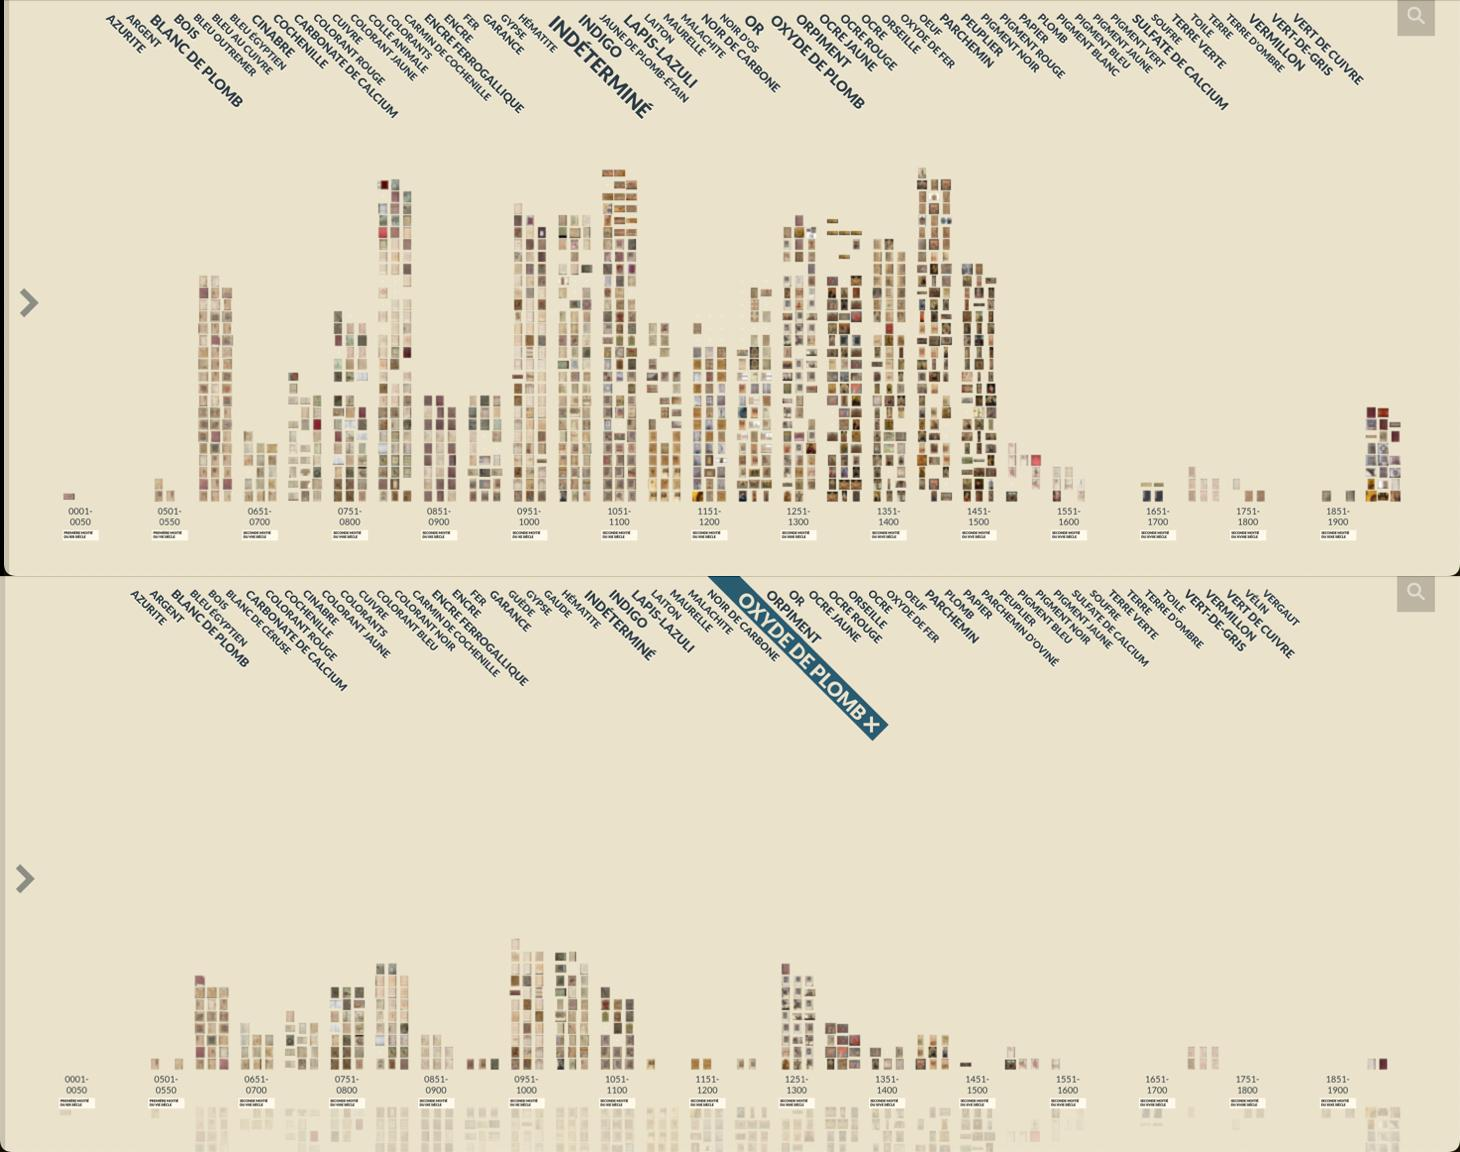
\includegraphics[width=\textwidth]{./textes/chap3/vikus-dyna.jpg}
	\caption{Déplacement d'icônes dans Vikus}
	\label{fig:info}
\end{figure}

Le filtrage repose sur deux paramètres, des séquences chronologiques et des thèmes spécifiques. Les données suivent une distribution temporelle dans \indexmot{VIKUS}. Cette \indexmot{chronologie} doit faciliter la compréhension d’un contexte historique et de tendances au fil du temps. La difficulté, pour un corpus comme le nôtre, réside dans la fragmentation et l’incertitude des datations. Les enluminures des manuscrits ne peuvent être que difficilement datées. Elles font bien souvent l’objet d’une estimation, d’une approximation chronologique afin de proposer un contexte historique vraisemblable. Parfois, l’ordre de grandeur est seulement de quelques années, parfois il est de plusieurs décennies. Dans une \indexmot{frise chronologique} classique, ces incertitudes sont contournées par la figuration de jauges, de segment qui indiquent les bornes de la datation. Une telle approche n’est pas possible sur \indexmot{VIKUS}. Les datations sont elles-mêmes des entités et pas seulement des valeurs. Elles ne peuvent pas se chevaucher ou se croiser. Chaque datation doit avoir une valeur unique et chaque feuillet doit avoir une seule datation. Dès lors, un certain arbitraire s’impose dans l’assignation d’un contexte de création à une enluminure.\par
L’autre difficulté réside dans le découpage de la \indexmot{chronologie}. Les feuillets apparaissent par colonne au-dessus de leur datation~: plus ces dernières seront nombreuses, plus les colonnes seront petites et peu lisibles~; moins les datations seront nombreuses, plus les résultats perdent en sens, diluant les mouvements artistiques dans de grandes ères historiques. Il me semble qu’une répartition par demi-siècle est, au regard du corpus, la meilleure division possible. Elle permet une \indexmot{visualisation} lisible et fluide, tout en n’élargissant pas exagérément les séquences chronologiques. Elle a, néanmoins, l’inconvénient de rapprocher artificiellement des productions séparées parfois de près de quatre décennies et d’en séparer d’autres proches de seulement quelques années. Ainsi, sur une même colonne, pourraient figurer des enluminures des années 1350 et 1390, mais elles seraient séparées de celles du début de la décennie 1400. Il y a là un biais propre à \indexmot{VIKUS} que je ne peux contourner. Néanmoins, la \indexmot{chronologie} de plus d’un millénaire sur laquelle reposent les analyses effectuées permet de lisser ce défaut, lorsque le regard est porté sur un temps long.\textit{Voir la figure 3.2.}\par
\begin{figure}[p]
	\centering
	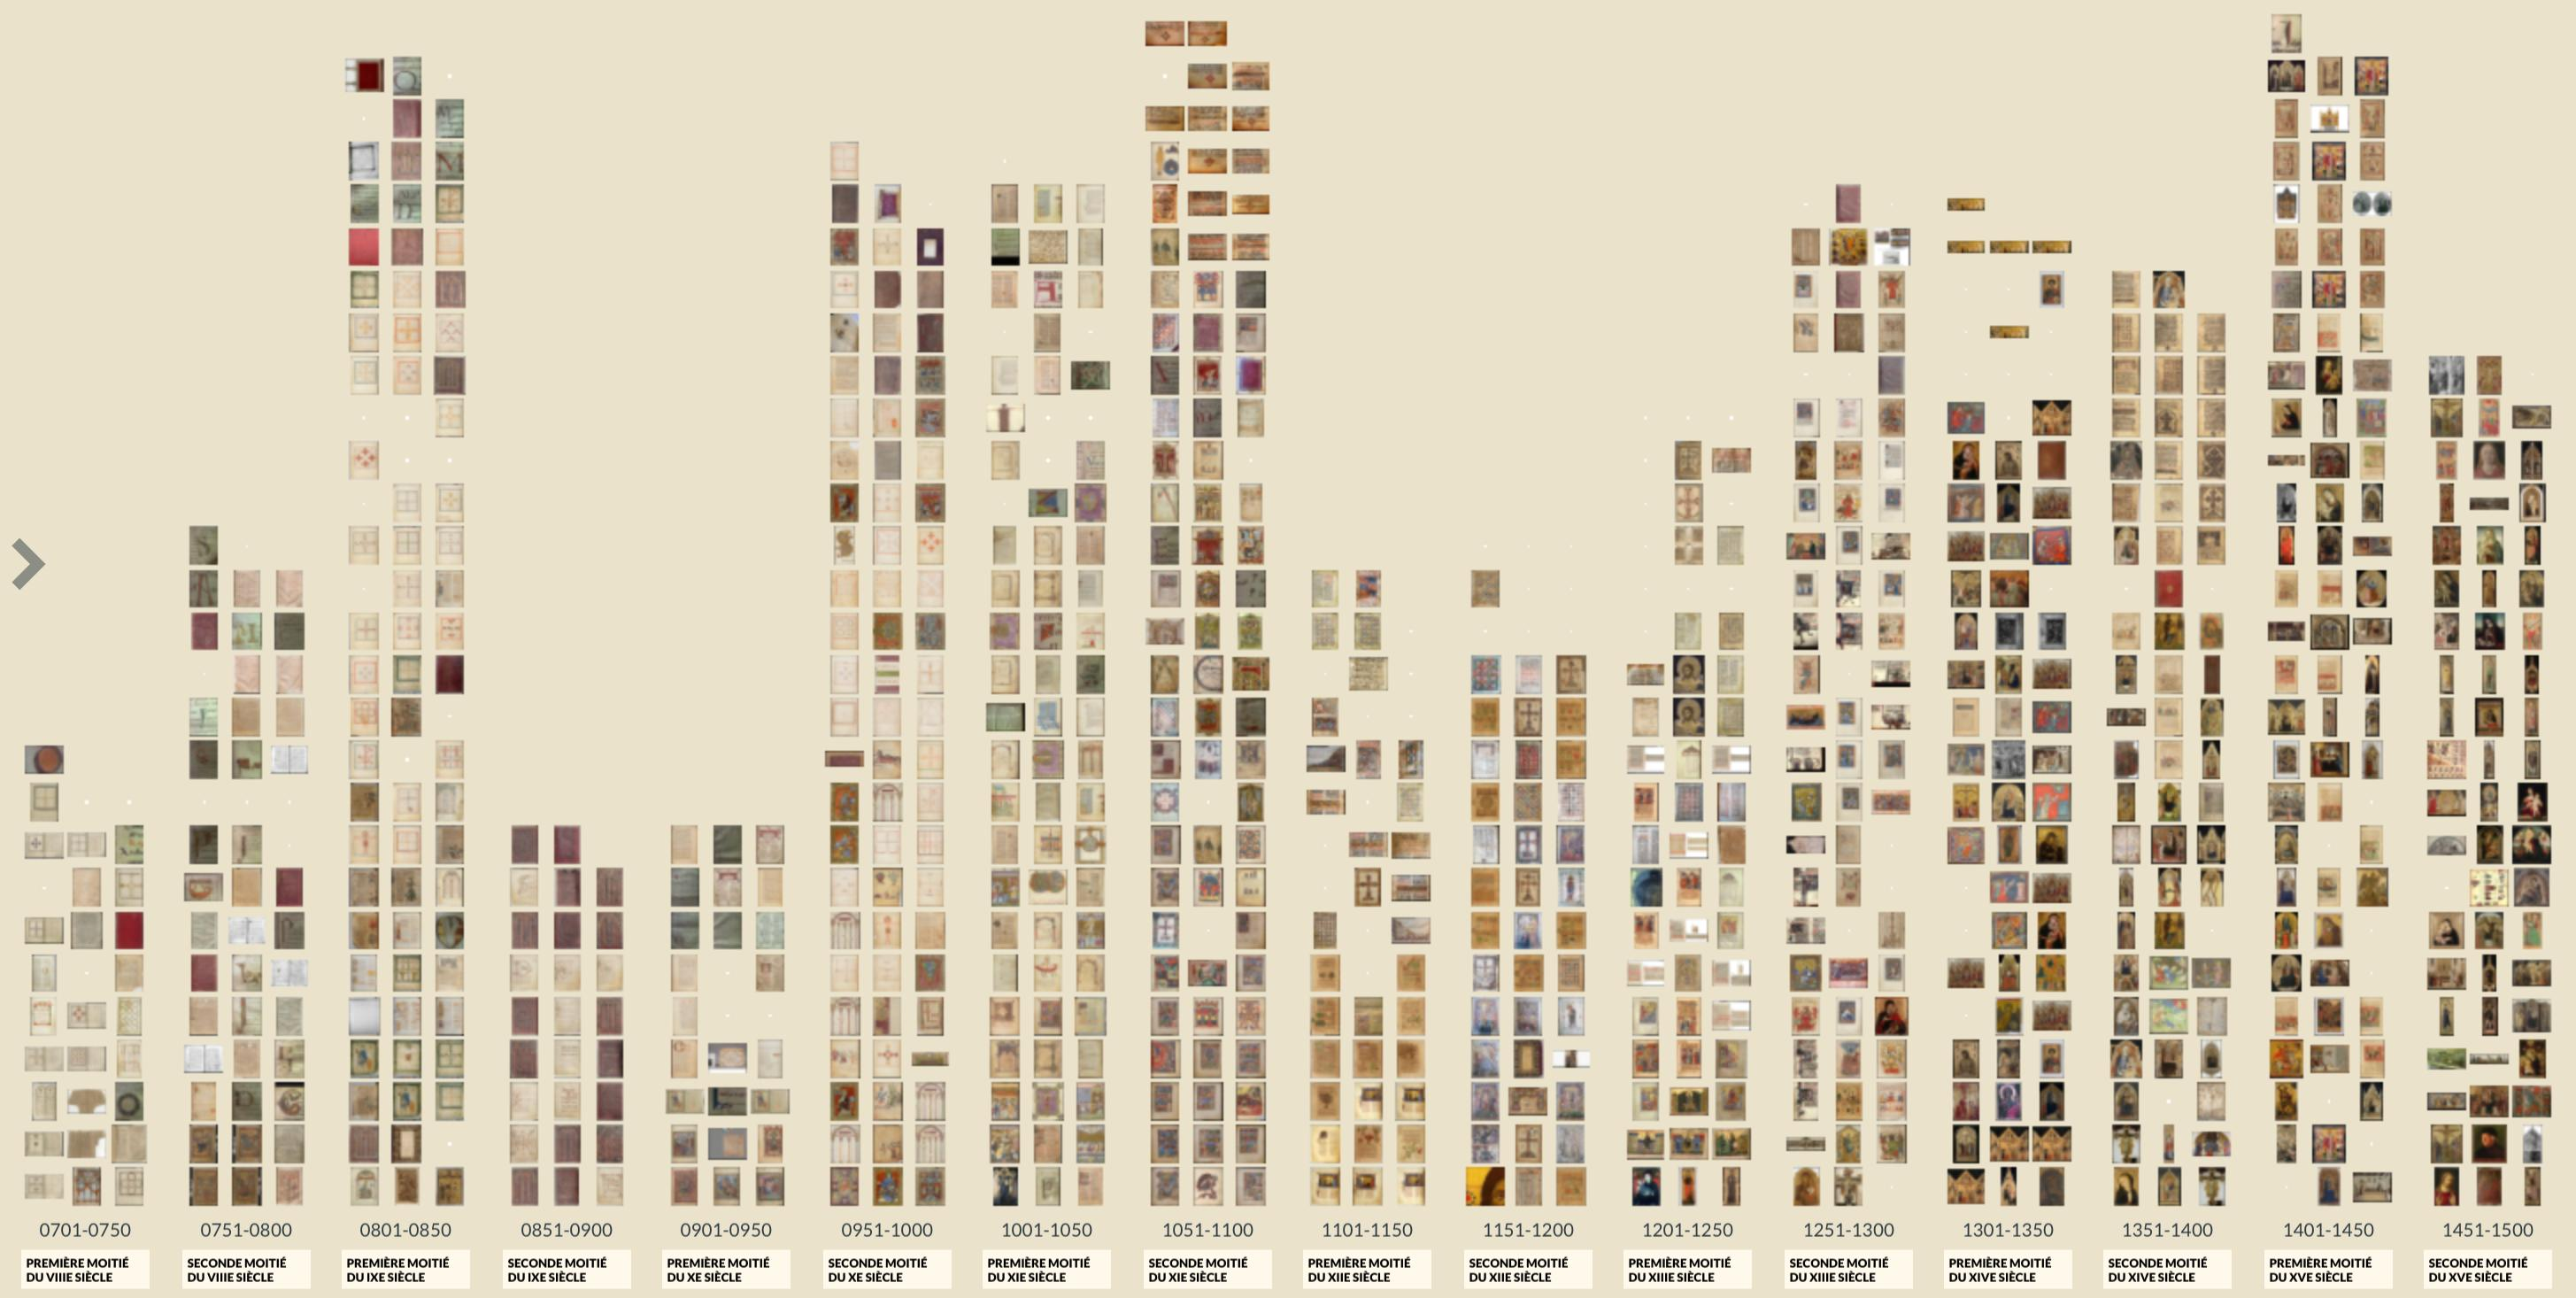
\includegraphics[width=\textwidth]{./textes/chap3/vikus-chrono.jpg}
	\caption{Les séquences chronologiques dans la frise}
	\label{fig:info}
\end{figure}

La seconde variable repose sur l’ontologie des matériaux. Comme pour la \indexmot{carte interactive}, le matériau est à nouveau le pivot des résultats obtenus. La navigation se fait à travers les mots-clefs, isolés et rangés alphabétiquement, présents dans la partie supérieure de la fenêtre. La taille de ces valeurs varie en fonction de leur occurrence~: si un matériau apparaît fréquemment dans le corpus, il aura une police supérieure à celle d’un autre plus rare. Le filtre par matériau proposé dans cette \indexmot{visualisation} permet de combiner les valeurs, ce qui n’est pas le cas sur la \indexmot{carte interactive}. La recherche s’affine et il est possible d’interroger la co-présence de matériaux au sein d’un même feuillet. Dans le cas ci-dessous, la première recherche est faite sur la seule présence de cochenille, puis elle se précise dans un second temps avec celle d’orseille. Le résultat obtenu est une \indexmot{visualisation} très précise sur leur usage commun à partir de la seconde moitié du Xe siècle et qui demeure rare dans le temps.\textit{Voir la figure 3.3.}\par
\begin{figure}[p]
	\centering
	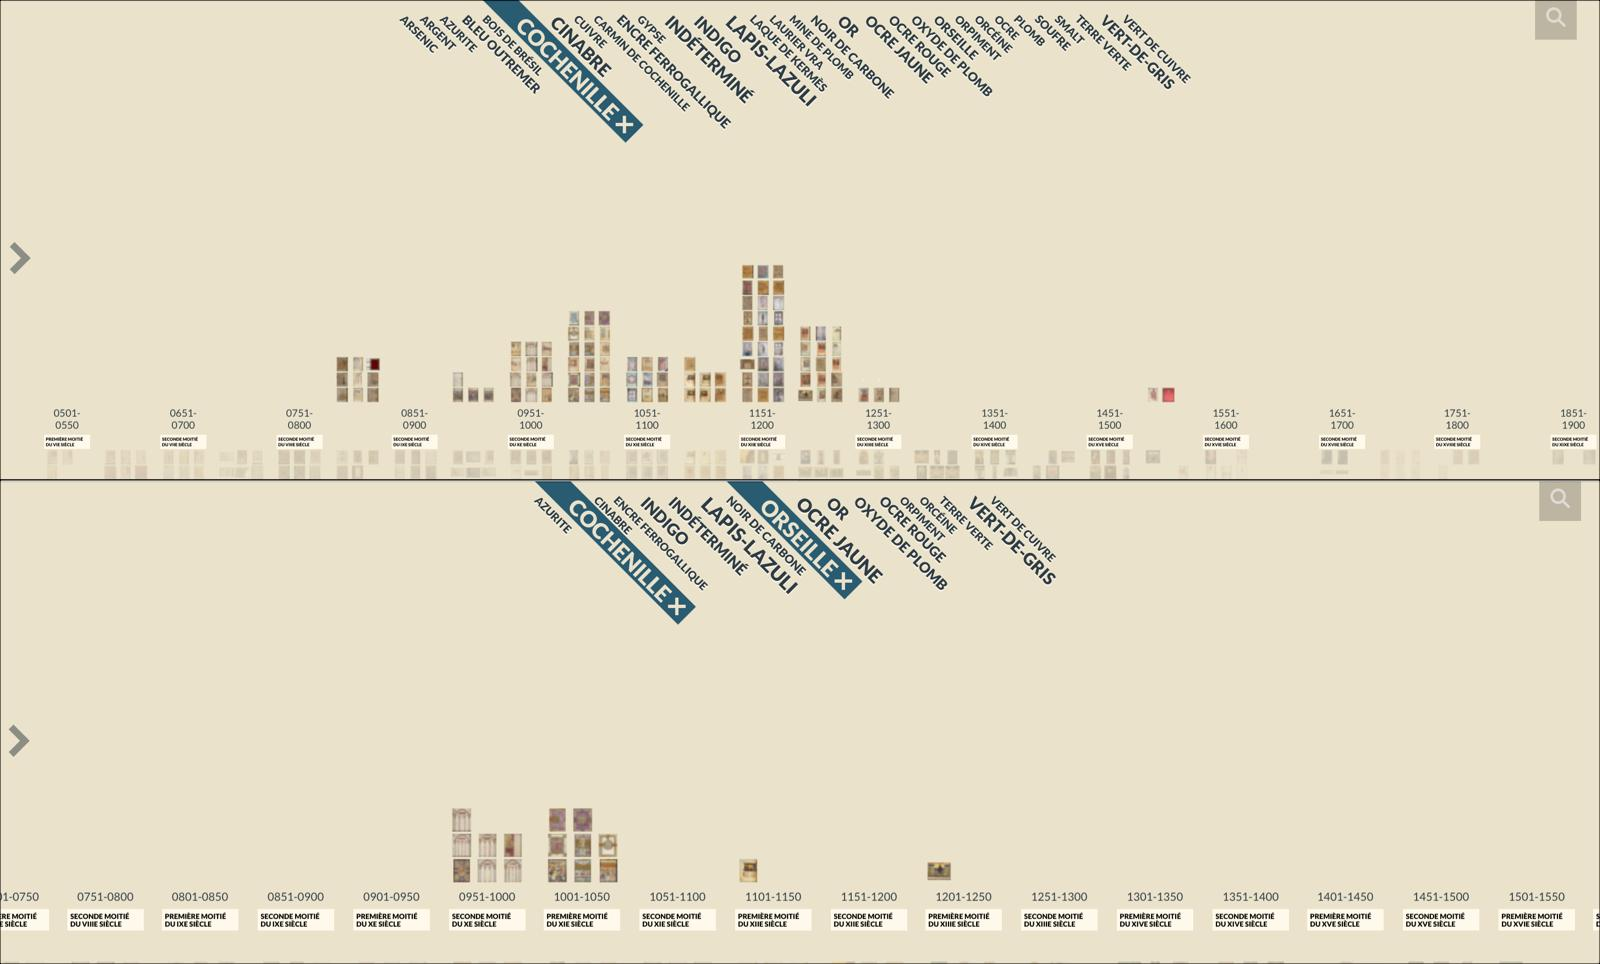
\includegraphics[width=\textwidth]{./textes/chap3/vikus-double.jpg}
	\caption{Co-présence de matériaux}
	\label{fig:info}
\end{figure}

Les \textit{artefacts}, comme les appelle Christopher Pietsch, qui sont traités par le logiciel, prennent l’apparence de l’image du feuillet. Elles se déplacent sur l’ensemble de l’interface selon le paramétrage du filtre. Avec un niveau de zoom suffisant ou avec un clic, l’interface fait apparaître une barre latérale à côté de l’image. Elle reprend les informations essentielles du feuillet. J’y fais figurer le titre de l’œuvre, les matériaux qui sont utilisés pour sa réalisation, les résultats des différentes analyses, son lieu de création ainsi que sa localisation actuelle. L’utilisateur a à sa disposition toutes les informations essentielles pour appréhender le manuscrit.\par

\begin{figure}[H]
	\centering
	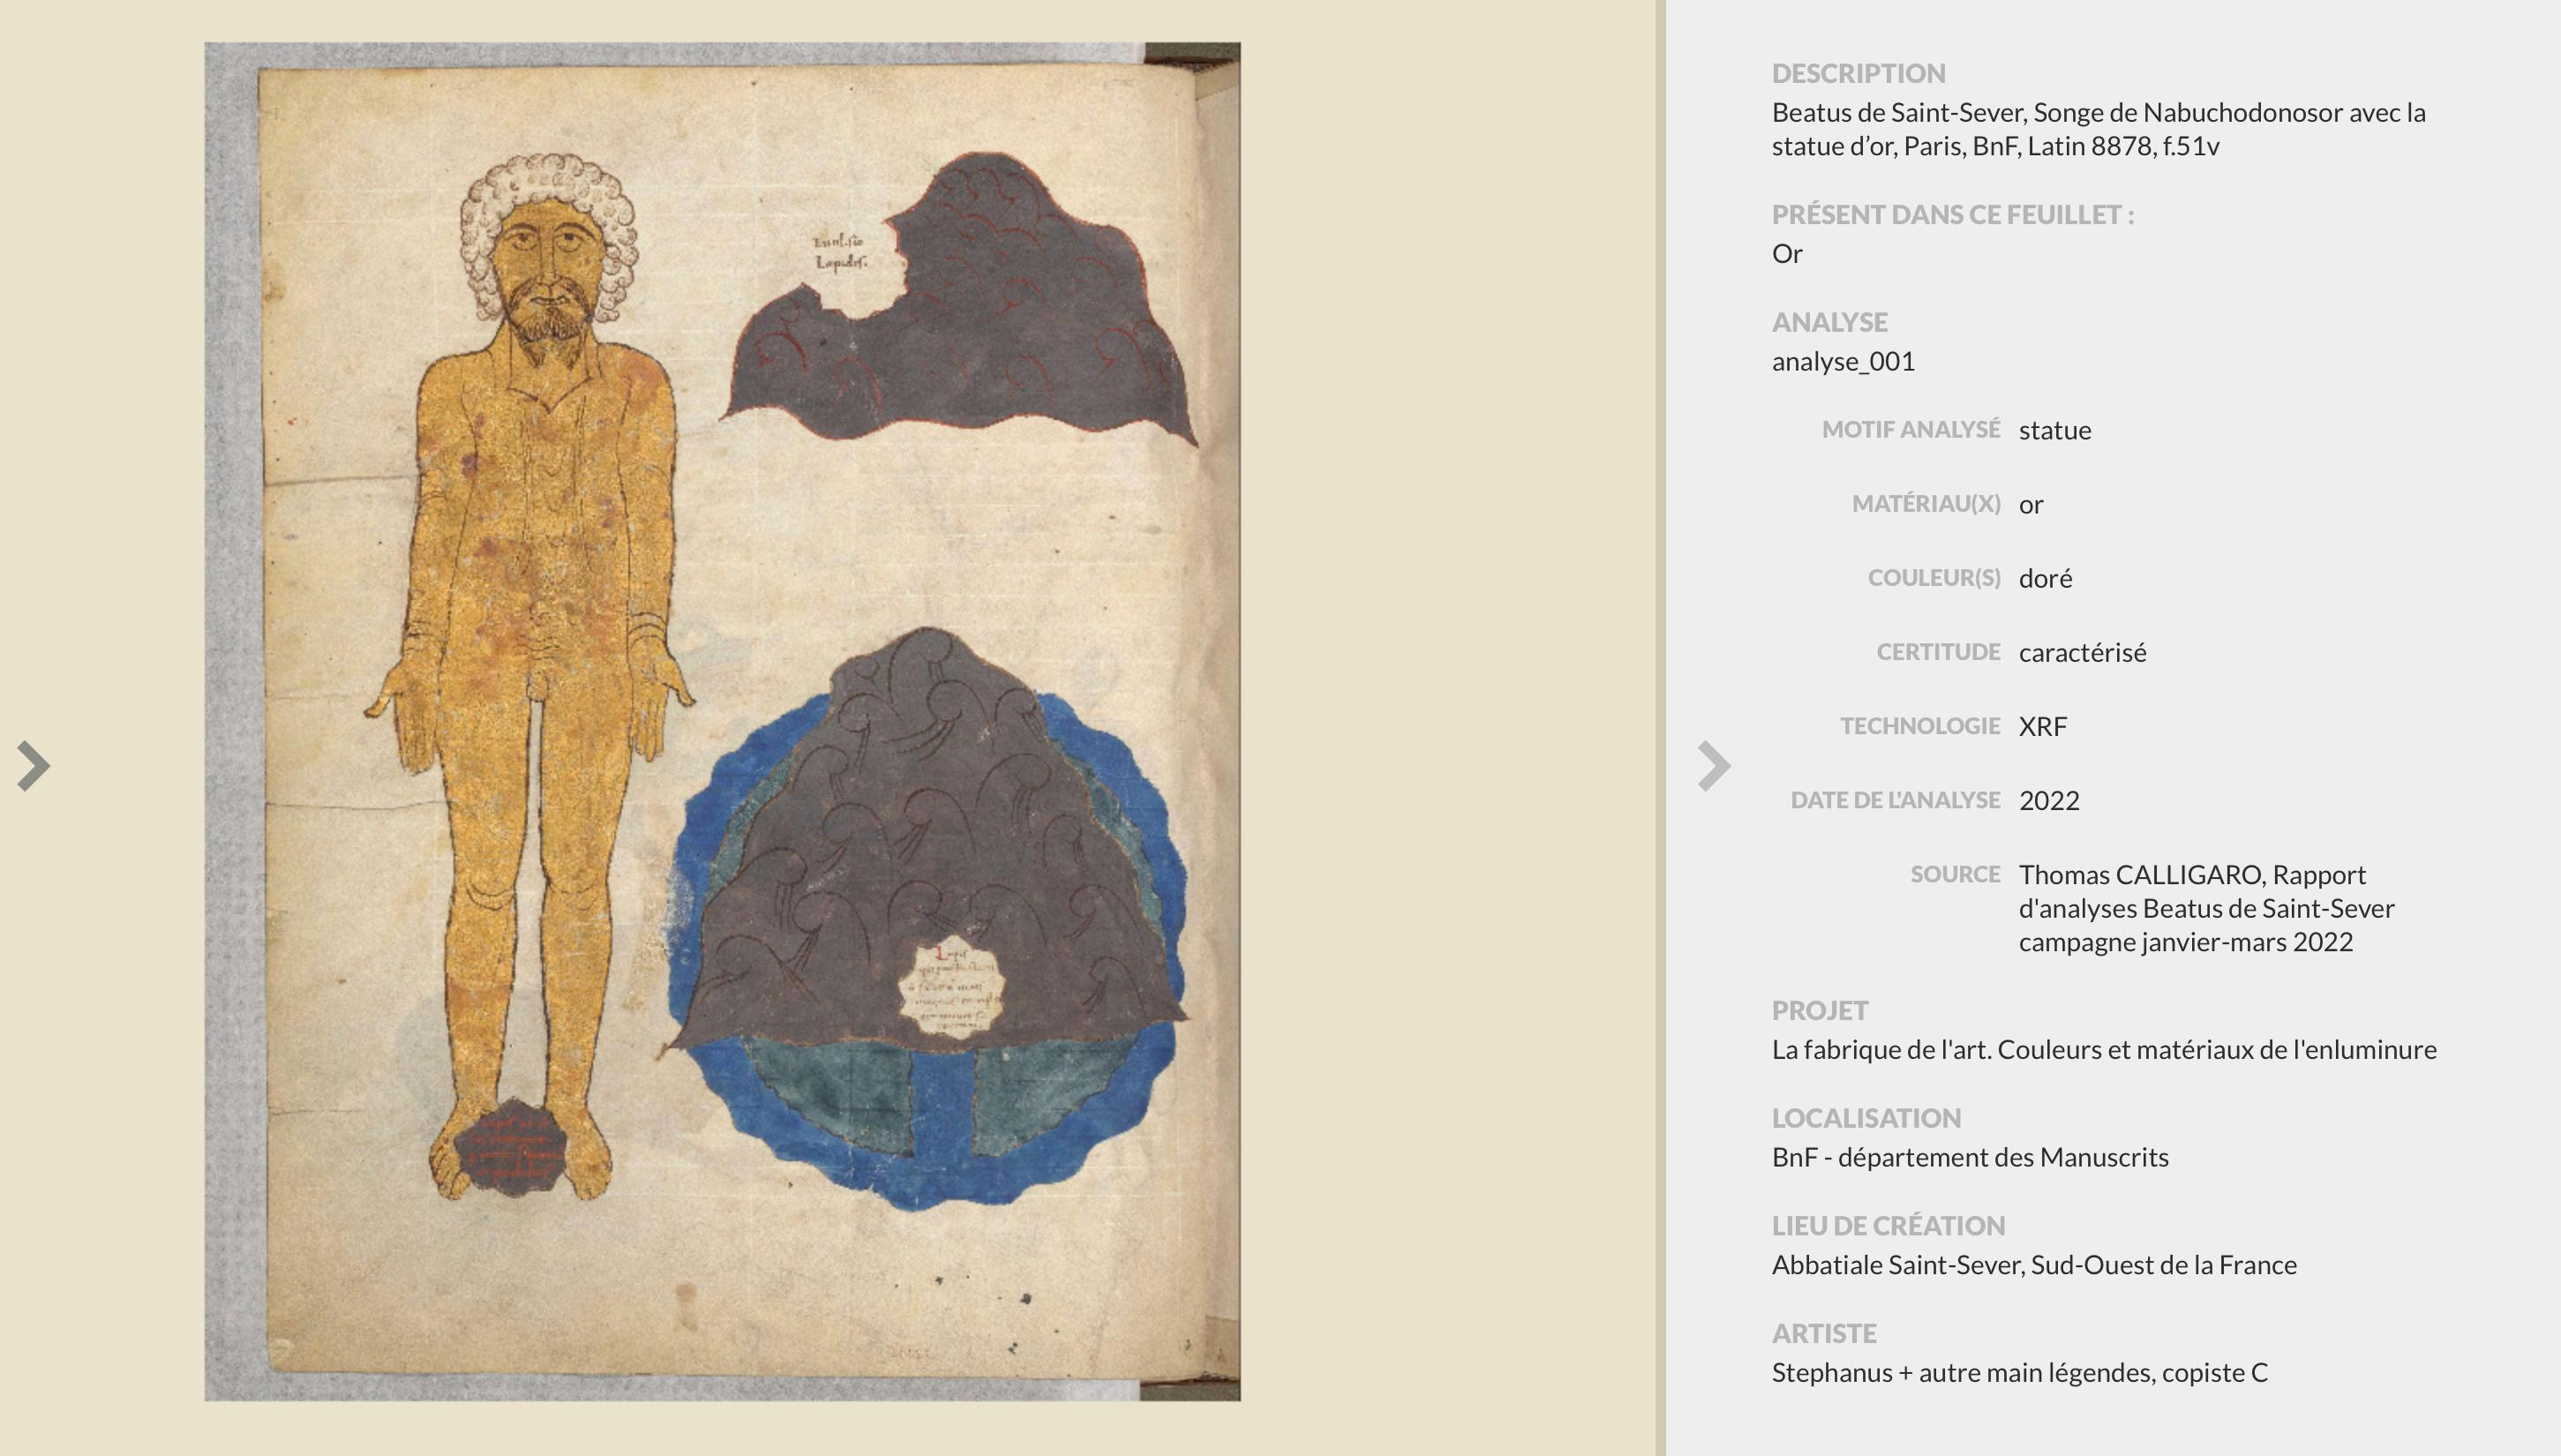
\includegraphics[width=\textwidth]{./textes/chap3/vikus-barre.jpg}
	\caption{Présentation des données sous Vikus}
	\label{fig:info}
\end{figure}

\indexmot{VIKUS} Viewer permet de travailler à partir de toutes les données entrées dans les deux bases du projet, materiality88 et 89. Celles-ci sont accessibles dans le champ supérieur de la fenêtre, qui permet la recherche en texte libre, que ce soit par le nom du manuscrit, de la couleur, du lieu de création ou de toute autre information. Si la \indexmot{visualisation} nécessite un certain appauvrissement de la \indexmot{chronologie}, toutes les autres données peuvent être encodées et reportées sans difficulté. Comme pour la cartographie interactive, l’essentiel de la transformation repose sur le langage Python.\newpage

\section{Traitement des données}

La \indexmot{visualisation} repose sur un fichier HTML qui est relié à des dossiers contenant du code JavaScript et du CSS\footnote{Le clonage du dépôt GitHub inclut également un dossier \enquote{font} pour les polices et un \enquote{image} pour les icônes utiles pour la mise en page.}. À cette architecture, il faut produire et ajouter un dossier \enquote{data}, qui est lu par les codes JavaScript et qui contient toutes les données qui sont traitées. La réalisation du dossier \enquote{data}, nous l’avons vu, se fait essentiellement à partir d’une imitation des exemples proposés. Dans le cas présent, je me suis inspiré du modèle réalisé pour les peintures de Van Gogh.\\\par 
Le travail repose sur la création de quatre fichiers de métadonnées qui décrivent la collection et les objets, et qui configurent la \indexmot{visualisation}. Il convient d’ajouter à ces fichiers une collection d’images, qui représentent les artefacts. Le premier fichier se nomme config.json. Il s'agit du fichier de configuration qui définit le nom du projet, les lien de données, les colonnes des artefacts, les styles et le contenu de la barre latérale qui détaille la collection.\par
Le data.csv contient toutes les informations de métadonnées pour chaque objet de la collection. Il a des champs obligatoires qui permettent de faire le lien avec les autres données. Les lignes doivent contenir au moins un identifiant, un mot-clef et une année. L’identifiant doit correspondre au nom de l’image qui sera produite par la suite. Par exemple, dans notre cas, l’identifiant fd106807-3864-4227-87ef-1ff82988616d correspond à l’image des \textit{Épîtres de saint Paul} (lettre ornée, Paris, BnF, Latin 10440, f.20r, f.20v). La complexité de l’identifiant peut surprendre, mais elle correspond en réalité à une simplification des données. Pour la préparation du fichier data.csv, je m’appuie sur le fichier préparé pour la cartographie. Afin de faire apparaître les résultats par feuillets, et non par analyses, je réalise un pivot de ces dernières sur chaque première ligne des feuillets, tout en les ordonnant selon une nouvelle numérotation. Ensuite, il suffit de procéder à un téléchargement des images en leur assignant le numéro de l’identifiant comme nom. En ce qui concerne les mots-clés, qui portent sur les matériaux, une concaténation des différentes analyses des feuillets, toutes présentes maintenant sur les mêmes lignes, permet de constituer la colonne. Il convient de réaliser un nettoyage des entrées ensuite, afin qu’elles puissent être correctement reconnues par le code JavaScript. Ensuite, la colonne ‘year’, elle aussi obligatoire, correspond à l’approximation par demi-siècle que je dois réaliser afin de proposer une \indexmot{visualisation} intelligible. Les autres colonnes du fichier data.csv correspondent à différents champs de métadonnées qui peuvent être personnalisés. Ici, nous retrouvons les informations qui correspondent au titre du feuillet, aux différentes analyses, aux lieu de création et de conservation, ainsi qu’au projet de recherche auquel il se rattache.\par
Le timeline.csv contient les informations pour la \indexmot{chronologie} affichée sous les années. Si l’année peut être un nombre ou une chaîne de caractère, elle correspond ici aux demi-siècles de la colonne ‘year’. Ensuite, le fichier doit contenir d’autres renseignements~: un titre de présentation sous les séquences chronologiques, un texte détaillé lorsqu’il y a un premier niveau de zoom, puis un texte supplémentaire lorsqu’il est zoomé au maximum. Ces éléments doivent contribuer à fournir un contexte historique à l’utilisateur lors de son exploration de la base. Cependant, avec une \indexmot{chronologie} \textit{artificielle} comme la nôtre, il n’est pas évident d’apporter des compléments d’informations sous les séquences chronologiques. J’ai simplement opté pour le fait de mettre en toutes lettres la période considéré~; ainsi la colonne \textit{0951-1000} est accompagnée de la précision \textit{Seconde moitié du Xe siècle}.\par
Enfin, le dernier fichier de métadonnées, info.md concerne les informations affichées sur le côté gauche lors de l'ouverture de la \indexmot{visualisation}. D’une écriture simple en Markdown, j’y fais apparaître une présentation simple et concise du projet de recherche et de la prise en main de l’interface.\\\par
À côté de ces quatre fichiers, la \indexmot{visualisation} repose sur la préparation et la configuration d’une collection d’images. Ces dernières doivent être téléchargées dans un seul dossier et nommées selon l’identifiant qui leur est assigné dans le fichier data.csv. Le traitement consiste en l’application du script vikus-viewer qui génère des sprites et des textures pour les différents niveaux de zoom.\par
En premier lieu, il faut cloner le dépôt et installer les dépendances~:\par
git clone https://github.com/cpietsch/vikus-viewer-script
cd vikus-viewer-script\par
npm install\\\par
Ensuite, le script est exécuté pour générer les textures et les sprites~:\par
vikus-viewer-script \enquote{/chemin/vers/les/images/*.+(jpg|jpeg|png)}\\\par
Le script crée un dossier de données pour les textures (1024 et 4096) ainsi qu'un dossier de sprites pour les spritesheets à l'intérieur du dossier actuel. \\\par
Les créations doivent être copiées à l’intérieur du dossier data, à côté des autres fichiers présentés précédemment.\par
Une fois que tous les liens sont bien vérifiés dans le config.json, il est possible de débuter la \indexmot{visualisation} avec un serveur web sur le fichier index.html.\newpage

\section{Chronologie et interprétation}

L'un des principaux avantages de l'utilisation de la \indexmot{chronologie} est qu'elle permet aux utilisateurs de comprendre les objets dans leur contexte historique. Les manuscrits sont, dans le cas présent, ordonnancés selon l’époque à laquelle ils ont été créés. La \indexmot{géographie}, les sujets iconographiques, les artistes et mêmes les couleurs ne jouent ici aucun rôle dans le classement. C’est une distribution temporelle stricte. Il s’agit, avec \indexmot{VIKUS}, de donner la primauté à une analyse historique du corpus. Nous pouvons en proposer quelques exemples.\par
Si nous revenons au cas de notre \indexmot{bleu égyptien} déjà évoqué au cours de ce mémoire, la \indexmot{frise chronologique} fait apparaître trois séquences à son utilisation dans les enluminures. La première est datée de la seconde moitié du VIe siècle, avec le \textit{Pentateuque dit d’Ashburnham}. Une deuxième séquence est très circonstanciée à la fin du VIIIe siècle, dans l’\textit{Évangéliaire de Charlemagne}. Sa dernière apparition est au XIe siècle, principalement dans le \textit{\indexmot{Beatus de Saint-Sever}}. Ces trois temps apparaissent sur la frise, sans qu’ils soient rapportés à d’autres variables que la date de réalisation et le matériau. La \indexmot{chronologie}, plus que toute autre forme de \indexmot{visualisation}, permet de représenter les discontinuités temporelles de l’emploi du \indexmot{bleu égyptien}. Les interruptions et les reprises successives dans l’utilisation du matériau apparaissent et invitent le chercheur à s’interroger sur les raisons artistiques, culturelles et matérielles de ces retours et disparitions au cours du temps.\par

\begin{figure}[H]
	\centering
	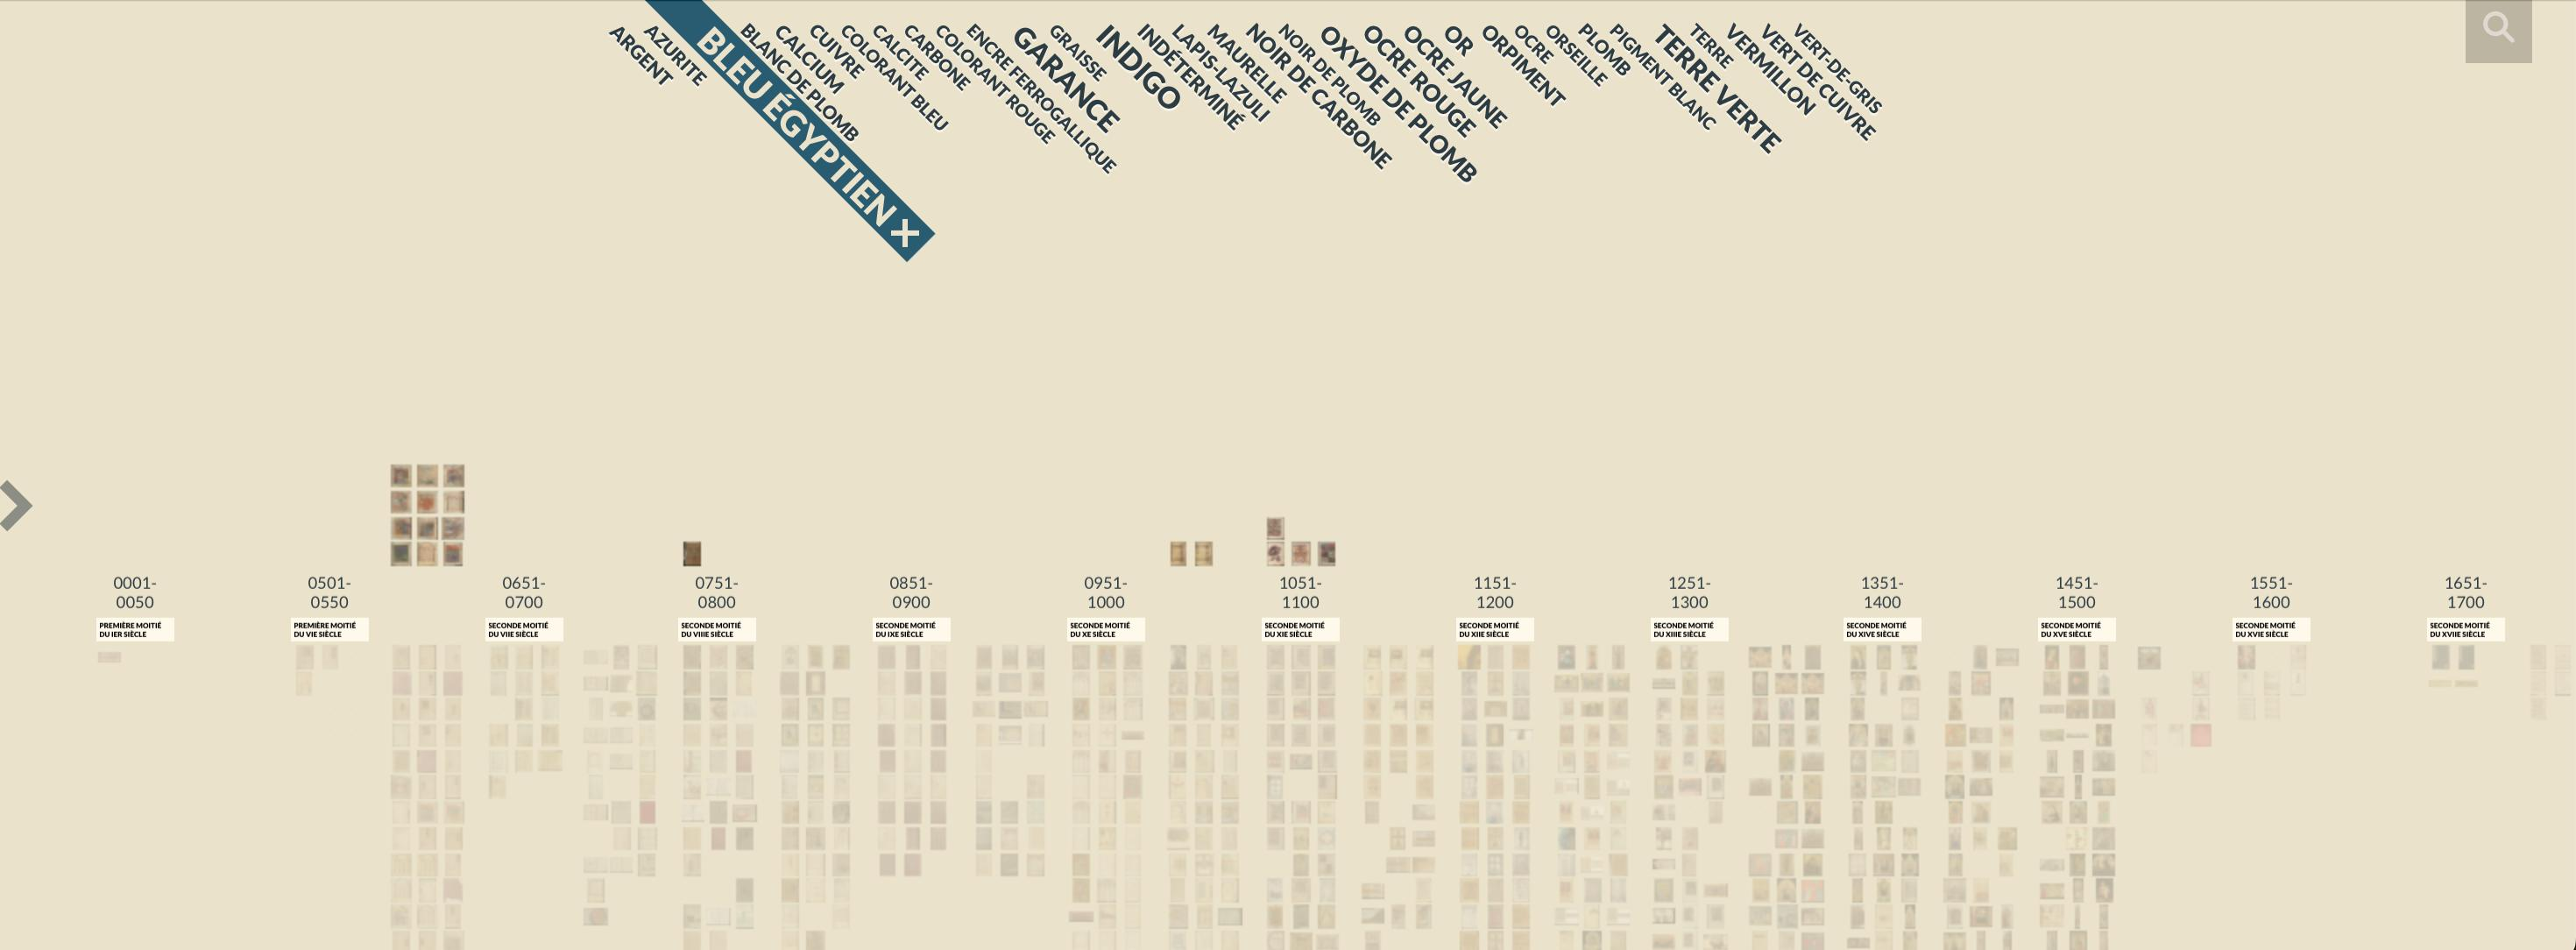
\includegraphics[width=\textwidth]{./textes/chap3/vikus-bleu-egy.jpg}
	\caption{Distribution temporelle du bleu égyptien}
	\label{fig:info}
\end{figure}

La \indexmot{chronologie} permet d'observer les évolutions et les tendances au fil du temps. Le deuxième exemple se sert de la recherche en texte libre que propose \indexmot{VIKUS} viewer pour porter un regard sur les contextes de production des enluminures. Ce champ permet d’interroger l’ensemble des données du fichier data.csv construit précédemment. En visualisant les occurrences du mot \textit{abbaye}, le résultat fait apparaître une longue séquence chronologique allant du VIIe siècle au XIe, avec une petite reprise aux alentours de l’année 1400. Une première hypothèque qui pourrait être formulée est celle de la mise en évidence, par la \indexmot{chronologie}, d’un déplacement dans le contexte de production du corpus analysé. Je n’évoque qu’une hypothèse, la base de données n’étant pas suffisamment fournie pour parvenir à une conclusion, mais la \indexmot{visualisation} invite à porter notre regard vers d’autres collections, afin de constater une même délocalisation de la production artistique, une même sortie des abbayes vers le monde.\par
La \indexmot{visualisation} reproduite ci-dessous rappelle que la \indexmot{chronologie} est aussi un discours sur le temps\footcite{toubkis_ordre_2004}. Les séquences de production des enluminures que nous avons définies, par demi-siècle, renvoie peut-être trop la \indexmot{chronologie} à un instrument taxinomique\footcite{certeau_ecriture_1975}. Avec une étude plus poussée des contextes de production de ces enluminures, il serait alors possible de proposer des \indexmot{chronologie}s-typologies sur \indexmot{VIKUS}, comme des emboîtements thématisés. Serait-il dès lors possible de recomposer un récit temporel et de concevoir comme séquence chronologique un \textit{temps de production abbatiale} par exemple?\par

\begin{figure}[H]
	\centering
	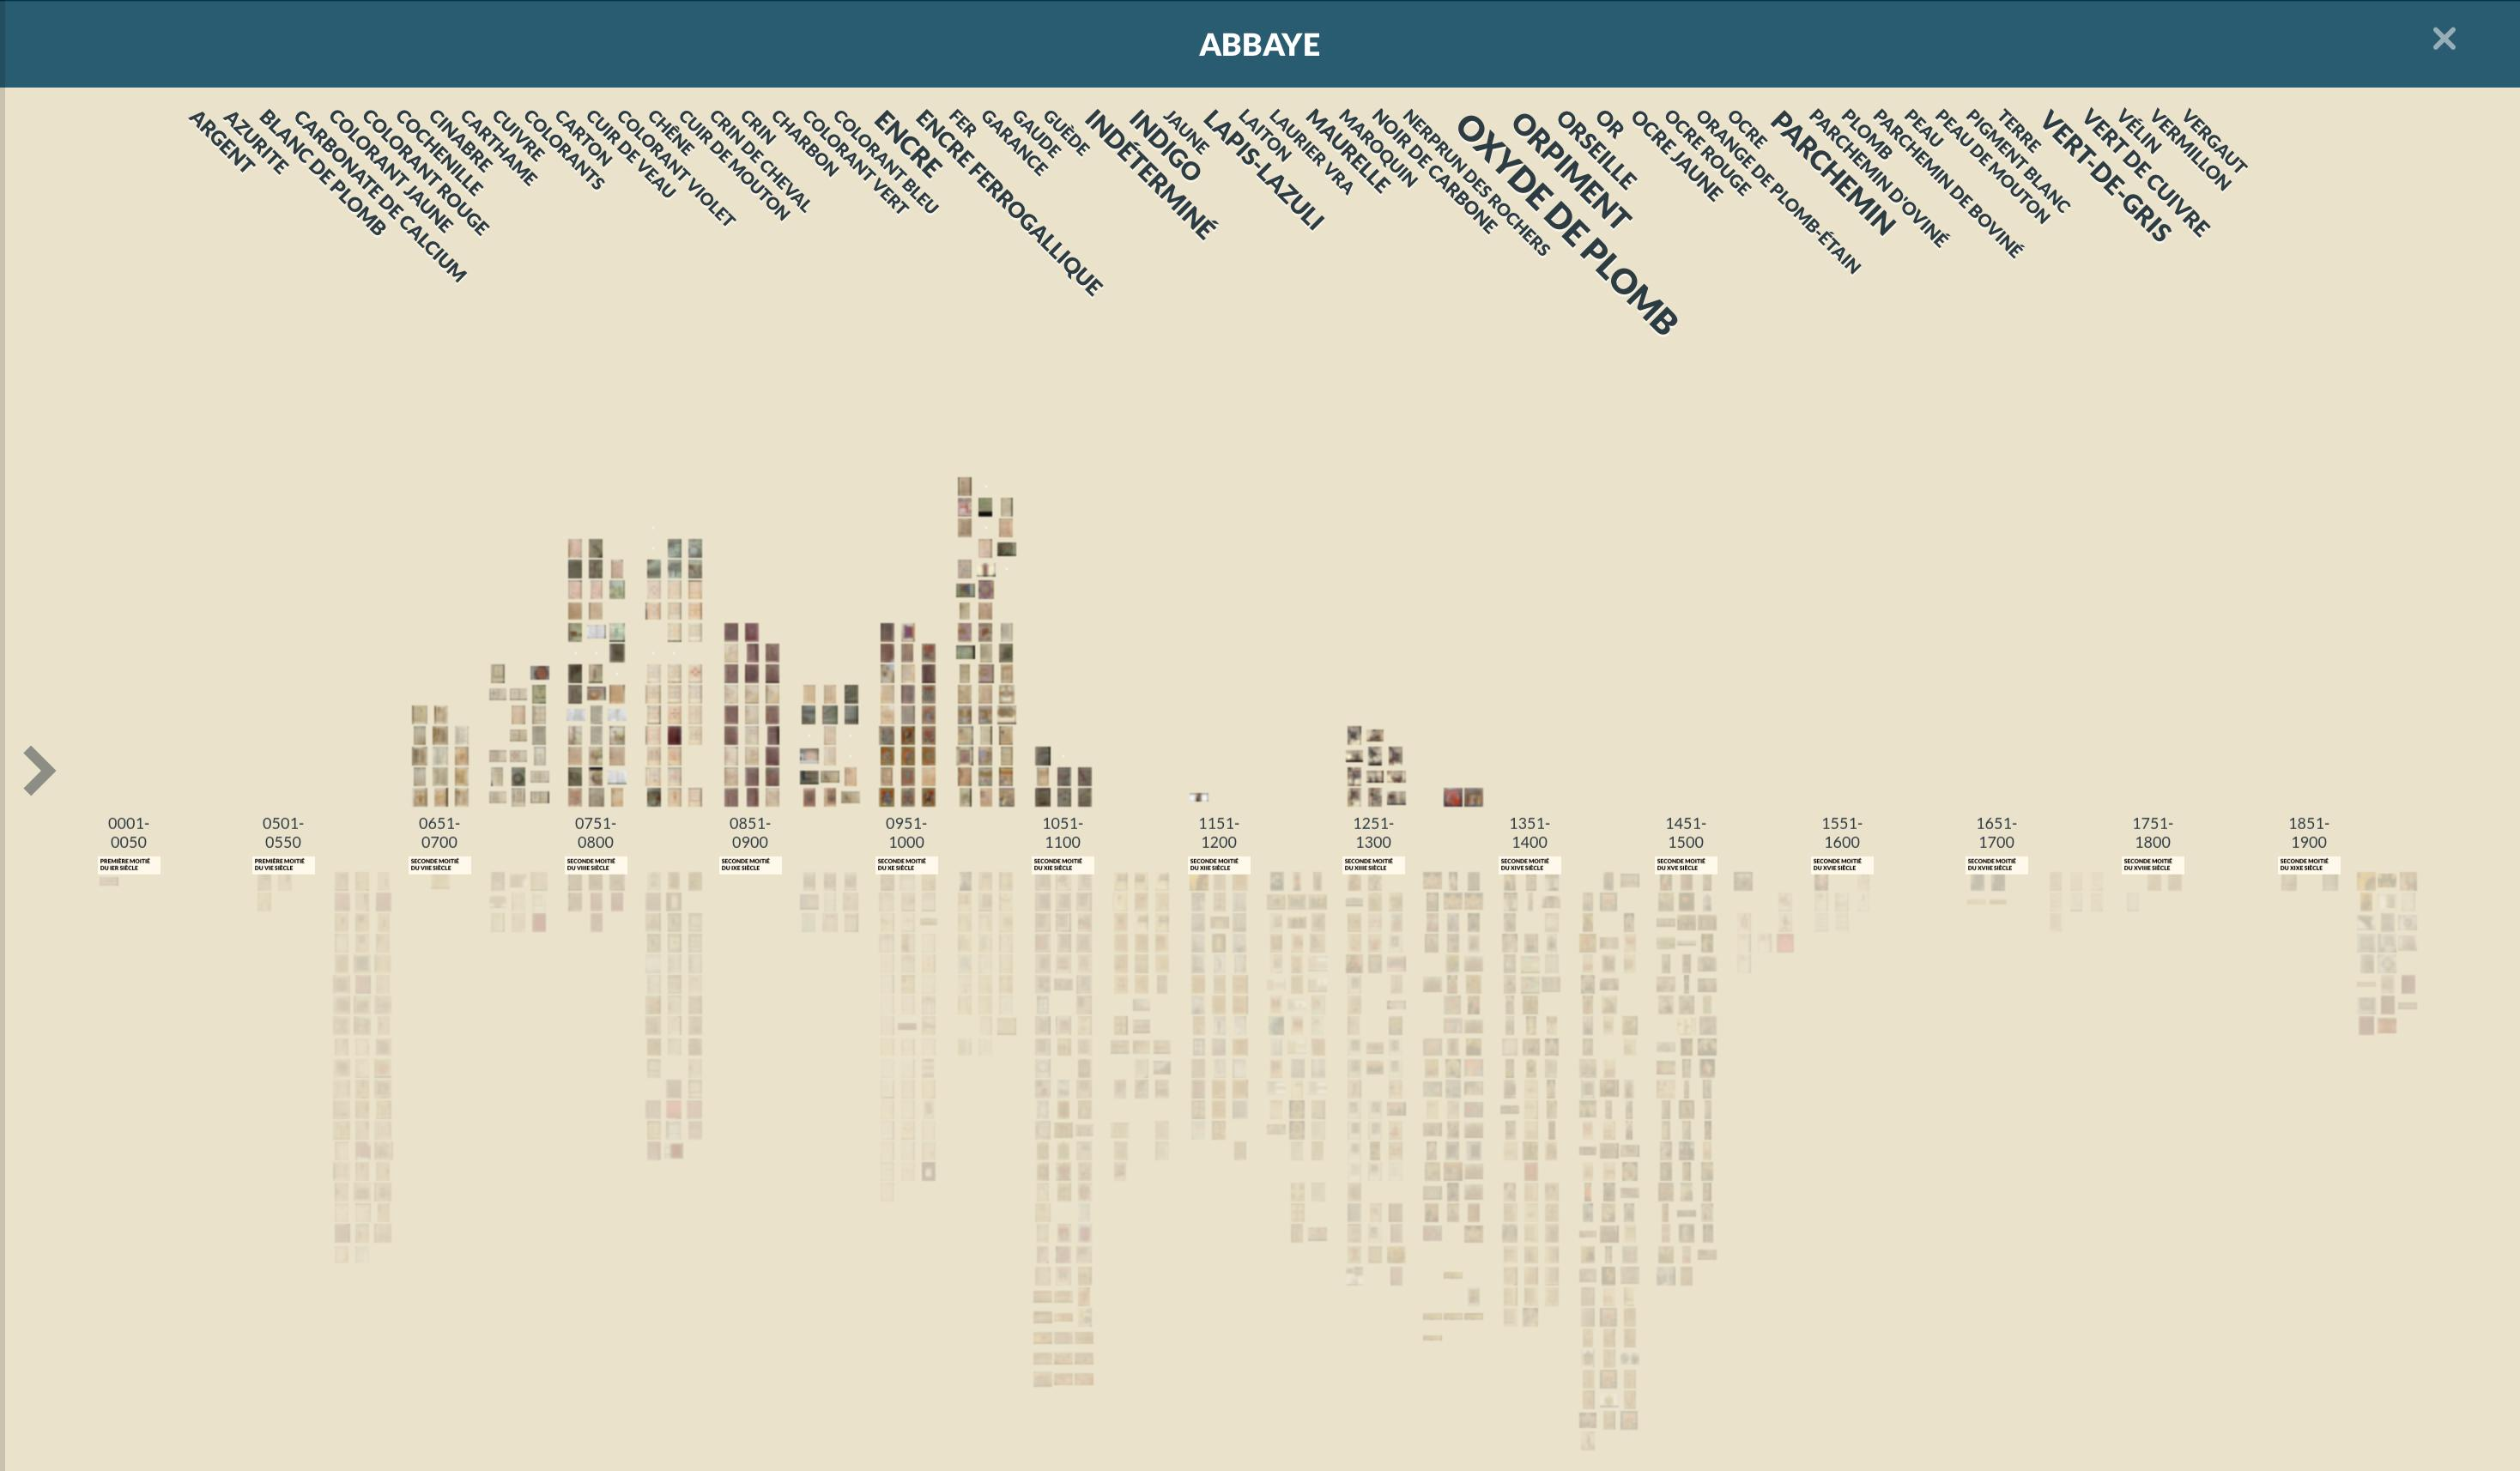
\includegraphics[width=\textwidth]{./textes/chap3/vikus-abbaye.jpg}
	\caption{Chronologie de la production abbatiale}
	\label{fig:info}
\end{figure}

\newpage
*\\\par
Ces exemples sont des parfaites illustrations des vertus heuristiques de certaines formes de \indexmot{visualisation} évoquées au cours de ce mémoire. Le brassage des données, selon des critères tantôt géographiques, tantôt chronologiques, permet l’observation de disjonctions et de continuités. Ces observations sont à la source de nouvelles analyses pour les chercheurs. \par
En somme, l'utilisation d'une \indexmot{chronologie} enrichie par des mots-clés, à l’image de celle proposée par \indexmot{VIKUS} Viewer, permet une exploration plus approfondie et contextuelle des données de la recherche. Elle offre une compréhension temporelle du corpus, elle met en lumière les évolutions et les tendances historiques, et elle facilite la comparaison selon des thèmes au fil du temps, ce qui peut être particulièrement précieux pour les chercheurs, les historiens et le grand public.


	
	\chapter{Annotations sémantiques d'images}
	Les deux projets de recherche, \enquote{La couleur~: artefacts, matière et cognition} et \enquote{La fabrique matérielle du visuel~: panneaux peints en Méditerranée}, ont chacune des entrées de leur base de données reliée à une image numérique. Il s'agit d'une photographie, en haute résolution, du feuillet de manuscrit ou du panneau qui est l'objet des analyses. Il y en a plus de mille cent. C'est un atout majeur du projet~: elles permettent non seulement de faire connaître au grand public des chefs-d'œuvre conservés dans les manuscrits, mais également de servir de supports aux analyses pour les chercheurs.\par
Le musée d’art et d'antiquités de l'université de Cambridge, le Fitzwilliam Museum, a proposé une valorisation de ses manuscrits enluminés à l'adresse suivante~: \url{https://www.fitzmuseum.cam.ac.uk/illuminated/}. À partir d'une petite sélection, les équipes du musée présentent les enluminures en haute résolution, avec des métadonnées descriptives et des points d'analyse sous forme d'annotations. Il me semble que le travail réalisé ici peut servir de modèle pour d'autres projets de recherche, comme ceux qui nous concernent aujourd'hui. Il est, d'une certaine façon, question de faire au cours de ce stage une démarche similaire avec des manuscrits sélectionnés par le département des manuscrits.\newpage

\section{Un fac-similé numérique}

L’idée est de travailler à partir des images numérisées des feuillets et de proposer des annotations qui pourront servir aux chercheurs. Une annotation est une information supplémentaire ajoutée à l'image, soit pour la décrire, soit pour y apporter des informations. Dans notre cas, il s’agit d’y renseigner les données de la base sur les analyses réalisées. Ces annotations se superposent à des images qui s’inscrivent dans un ensemble de protocoles, appelé IIIF.\par
L'International Image Interoperability Framework (IIIF) a été développé pour répondre à la nécessité d'un accès standardisé et interopérable aux images numériques dans le domaine des bibliothèques, archives et musées\footcite{noauthor_international_2024}. L’idée de ce consortium\footnote{Parmi les premières institutions à travailler sur les protocoles IIIF, nous pouvons citer la Bibliothèque Bodleian de l'Université d'Oxford, la Bibliothèque de l'Université de Stanford ou encore la British Library.}, fondé au cours de la décennie précédente, est de changer la manière dont les images numériques sont partagées et utilisées. Les images seront numérisées une seule fois en haute résolution par une institution, et elles seront déposées sur une plateforme, d’où elles pourront être appelées par n’importe quel utilisateur, selon son besoin spécifique. Ainsi, pour ce qui est des images des manuscrits que nous souhaitons valoriser, il suffit d’appeler les images numériques présentes sur la plateforme Gallica. L’interopérabilité permet de ne plus se soucier du processus de numérisation, déjà assuré par d’autres services.\\\par
Avec les protocoles qui définissent IIIF, les images sont non seulement consultables par n’importe quelle application ou logiciel compatible, mais elles sont également manipulables et annotables\footcite[La présentation de IIIF qui suit doit beaucoup à deux sites internet de vulgarisation. Le premier est le workbench de Glen Robson, le second est la documentation proposée Régis Robineau pour Biblissima][]{robson_iiif_nodate,biblissima_quest-ce_nodate}. Pour ce faire, il faut passer par des interfaces de programmation d’application (API). Dans le cadre de IIIF, ces dernières sont doubles. Elles concernent aussi bien l’image en elle-même, appelée l’API image, que sa présentation, c’est-à-dire avec ses métadonnées, appelée l’API présentation.\par
L’API image permet d’appeler les pixels d’une image et de manipuler cette dernière à distance à travers une syntaxe d’URL standardisée. Le modèle de toute API image suit ce schéma~:\par
{scheme}://{server}{/prefix}/{identifier}/{region}/{size}/{rotation}/{quality}.{format}\par
Pour les images que j’appelle sur Gallica pour les manifestes du projet, elles deviennent par exemple~:\par 
https://gallica.bnf.fr/iiif/ark:/1214/btv1b6000718s/f1/full/full/0/native.jpg\par
Il est dès lors possible de changer de région, de taille, de rotation, de qualité et de format selon les besoins spécifiques.\par
De son côté l’API présentation est décrite par Régis Robineau comme celle qui \enquote{spécifie les métadonnées (descriptives, structurelles, techniques) nécessaires à la présentation d’un objet numérique dans une interface. Toutes ces informations sont contenues dans un fichier appelé \enquote{manifeste}, une sorte d’enveloppe virtuelle formant l’unité de distribution élémentaire dans l’univers IIIF\footnote{https://doc.biblissima.fr/iiif/introduction-iiif/\#principe}. C’est en général ce fichier que vont manipuler les logiciels pour interagir avec une ressource, la visualiser, ou la transférer vers un autre outil.}\par
Un manifeste IIIF peut être un fac-similé numérique d’un objet physique (livre, manuscrit, périodique, carte, peinture, photographie, partition, monnaie, objet archéologique, archive sonore, captation vidéo, etc.), mais aussi un objet virtuel et composite constitué d’une série d’images ou d’autres médias rassemblés à des fins scientifiques ou pédagogiques, et pouvant provenir de différentes collections\footnote{https://doc.biblissima.fr/iiif/introduction-iiif/\#principe}. Dans le cas présent, les manifestes produits pour le stage s’apparentent à la première catégorie. Il s’agit d’un fac-similé numérique de manuscrit avec quelques annotations supplémentaires.\par
Le schéma ci-dessous, qui est proposé dans la documentation Biblissima, reprend les principales composantes d’un manifeste IIIF et permet de s’en faire une idée plus juste.

\begin{figure}[H]
	\centering
	\includegraphics[scale=0.19]{./textes/chap4/schema-iiif.jpg}
	\caption{Structure d'un manifeste IIIF}
	\label{fig:info}
\end{figure}

Les manifestes peuvent être affichés avec des visualiseurs IIIF. Ils proposent à l’utilisateur une expérience de \indexmot{visualisation} riche, s’appuyant sur l’ensemble des informations contenues dans les manifestes, au format JSON-LD. Les deux images ci-dessous permettent d’illustrer où sont mobilisées les deux API image et présentation dans un visualiseur comme Mirador~2. \par

\begin{figure}[H]
	\centering
	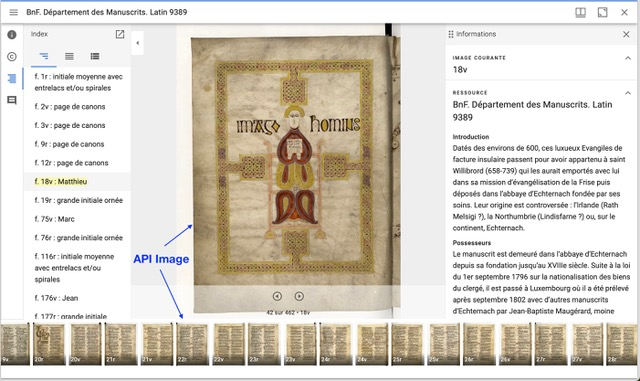
\includegraphics[scale=0.6]{./textes/chap4/mirador-api-image.jpeg}
	\caption{API Image}
	\label{fig:info}
\end{figure}
\begin{figure}[H]
	\centering
	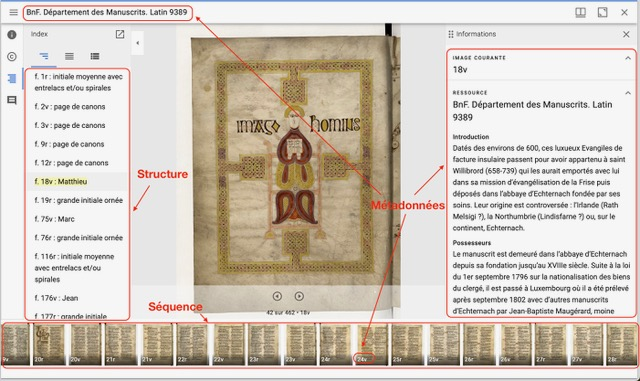
\includegraphics[scale=0.6]{./textes/chap4/mirador-api-presentation.jpeg}
	\caption{API Présentation}
	\label{fig:info}
\end{figure}

\newpage

\section{Enrichir une image numérique}

Les manifestes édités sont, je l’ai écrit précédemment, en quelque sorte un fac-similé numérique de manuscrit, avec quelques annotations supplémentaires. L’édition doit se faire au plus près de la version d’origine du manuscrit. Pour ce faire, et pour nos manuscrits, le point de départ est la bibliothèque numérique Gallica. La plateforme Gallica contient non seulement la numérisation de millions de documents de la \indexmot{Bibliothèque nationale de France}, mais elle donne également accès à une API qui permet de récupérer des manuscrits numérisés avec leur manifeste IIIF. Ces derniers permettent de récupérer tous les feuillets du document en haute résolution, ainsi que ses métadonnées descriptives et de séquences. Si je prends l’exemple du manuscrit Arabe~5847, Gallica propose l’intégralité de sa numérisation (avec les pages de couverture, pages de garde, contreplats et même le dos) dans le manifeste https://gallica.bnf.fr/iiif/ark:/12148/btv1b8422965p/manifest.json. Ce dernier contient également toutes les séquences du manuscrit, un titre pour tous les feuillets renseignés, qu’ils soient recto ou verso. Cette récupération auprès de Gallica permet de disposer du manuscrit Arabe~5847 en haute résolution et de travailler à la personnalisation du manifeste à partir de 9~292 lignes de JSON-LD déjà écrite par la plateforme.\par
Pour personnaliser le fac-similé numérique, il faut lui attribuer un nouvel identifiant unique. Chaque manifeste ne peut avoir qu’un seul identifiant. Pour différencier le travail qui sera réalisé sur le manuscrit de ce que propose Gallica, il convient donc de le rééditer sous un autre nom. La Bibliothèque Bodleian de l'Université d'Oxford met à la disposition du public un outil en ligne pour aider à la réédition. Il se trouve à l’adresse~: https://digital.bodleian.ox.ac.uk/manifest-editor/\#/?\_k=xjzu5x. L’éditeur permet de travailler soit à partir d’un nouveau manifeste, soit de reprendre un préexistant en le modifiant et en lui attribuant un nouvel identifiant. Dans notre cas, il suffit d’importer le canevas du manuscrit qui est renseigné sur Gallica. Ensuite, il est possible de personnaliser les métadonnées directement sur le site internet. Si les métadonnées descriptives de notre fac-similé numérique sont proches de celles de la plateforme de la BNF quant au titre, son introduction, son historique ou encore sa description technique, elles diffèrent au moment de les relier aux deux projets de recherche. Un paragraphe sur les matériaux utilisés dans le manuscrit est ainsi ajouté. En conséquence, lorsqu’une visionneuse IIIF interprétera le manifeste, il y aura, parmi les informations personnalisées, un premier résumé des résultats de la recherche.\newpage
\begin{figure}[H]
	\centering
	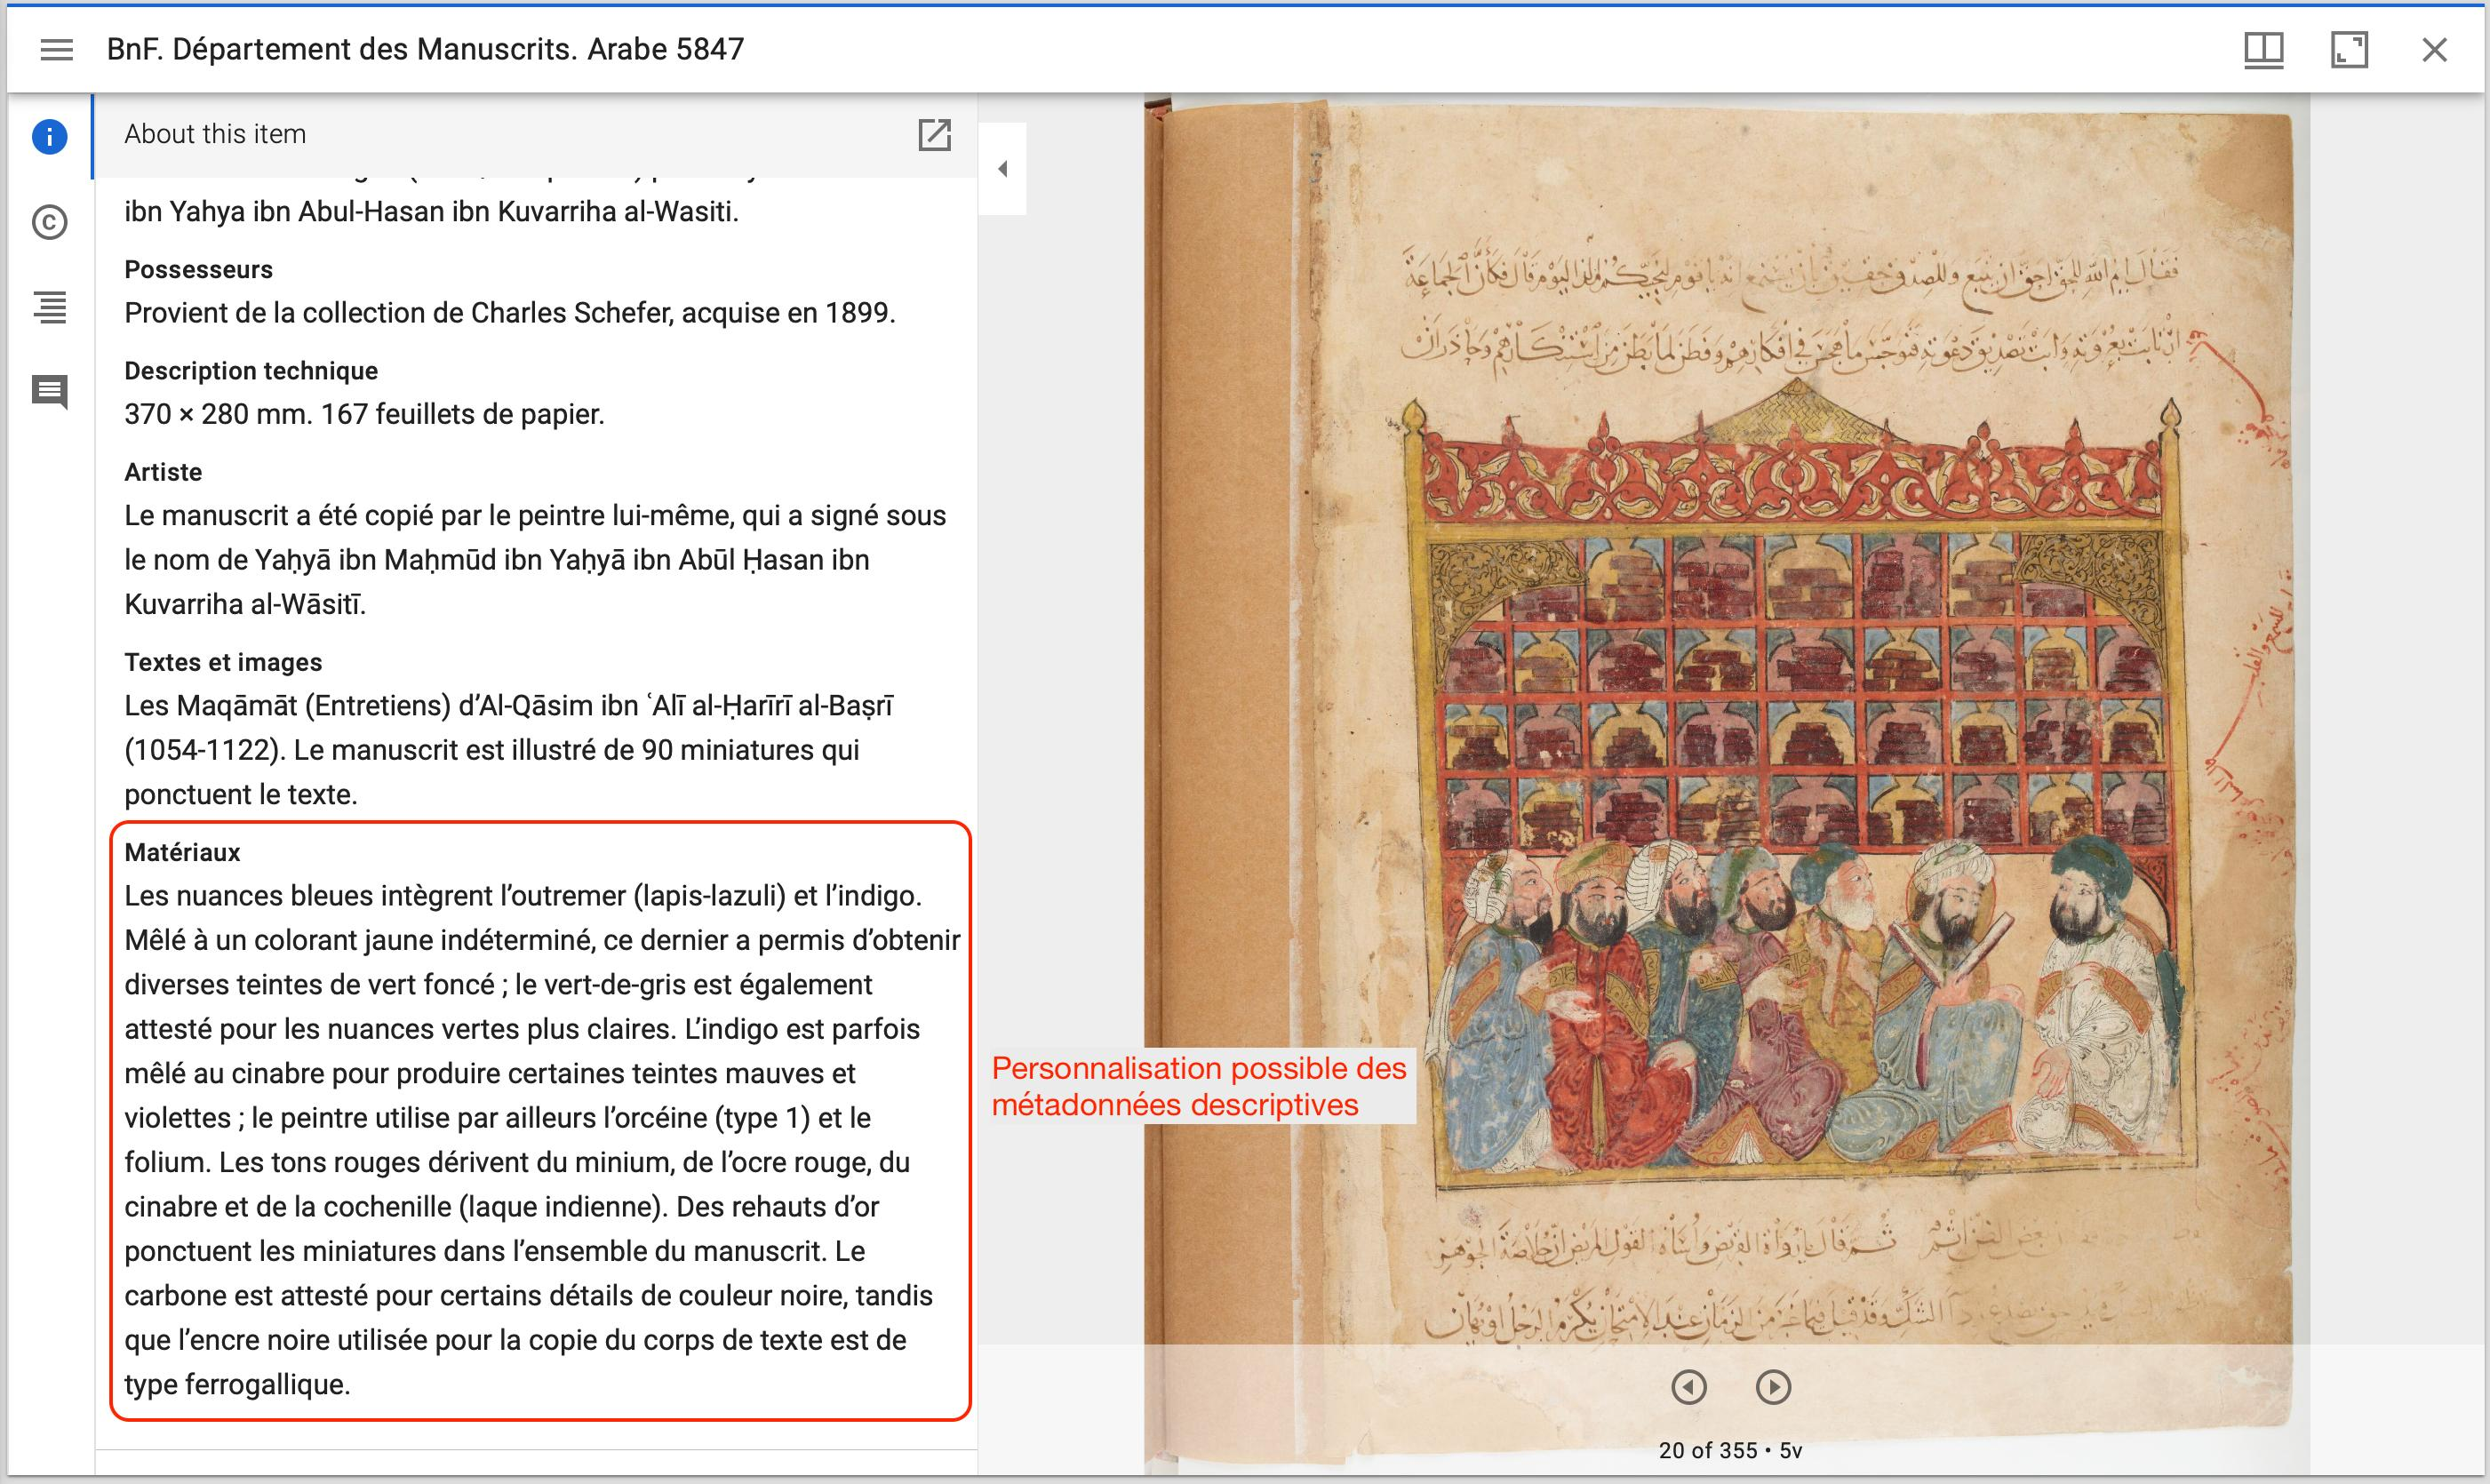
\includegraphics[width=\textwidth]{./textes/chap4/mirador-materiau.jpg}
	\caption{Personnalisation des métadonnées descriptives}
	\label{fig:info}
\end{figure}
Le fac-similé numérique peut être enrichi d’annotations\footnote{Il existe actuellement une dizaine de serveurs d’annotations IIIF. Les principales possibilités sont listées à l’adresse suivante~: https://github.com/IIIF/awesome-iiif?tab=readme-ov-file\#annotation-servers. Dans le cadre de ce stage, les annotations sont réalisées avec SimpleAnnotationServer (SAS), un serveur écrit en Java et développé par Glen Robson ( https://github.com/glenrobson/SimpleAnnotationServer).}. Ces dernières peuvent être invisibles, n’altérant pas la première lecture du manuscrit, ou visibles, permettant d’apporter des compléments d’informations. Les enrichissements possibles sur une image numérique sont nombreux. Il peut aussi bien s’agir de la transcription d’un document, d’un commentaire ou d’une analyse de contenu, ou encore de la mise en évidence d’une zone. Dans notre cas, il s’agit d’y renseigner les données de la base sur les analyses réalisées.\par
Les annotations IIIF suivent le Web Annotation Data Model\footcite{noauthor_web_2017}. Elles sont composées de deux parties. L’une renseigne le contenu de l’annotation, ce qui sera reporté sur l’image numérique~; l’autre indique la cible de l’annotation, le manifeste dont il est question et sa partie concernée par le commentaire. Une annotation simple a une structure standardisée composée de six points.\par
Structure d'une annotation~:
\begin{enumerate}
	\item @context~: il spécifie le contexte JSON-LD utilisé pour interpréter les données d'annotation.
	\item id~: un identifiant unique pour l'annotation.
	\item type~: le type de l'annotation, généralement il suffit d’indiquer "Annotation".
	\item motivation : la raison derrière l'annotation (par exemple, \enquote{commentaire}).
	\item target~: la ressource ou la partie de la ressource qui est annotée.
	\item body~: le contenu de l'annotation.
\end{enumerate}\par
De façon simplifiée, parce que celles réalisées sont finalement un peu plus complexes, une annotation sur le manuscrit Arabe 5847 peut répondre au schéma suivant~:
\begin{lstlisting}[language=json]
	{
		"@context": "http://iiif.io/api/presentation/2/context.json",
		"@id": "http://localhost:8888/annotation/1719318035104",
		"@type": "oa:Annotation",
		"motivation": ["oa:commenting"],
		"on": {
			"full": "https://gallica.bnf.fr/iiif/ark:/12148/btv1b8422965p/canvas/f34",
			"@id": "http://744902fa-f92b-4edf-b593-f9260051c14d"
		},
		"resource": {
			"chars": "<p>Motif : v&ecirc;tement, chausse dextre</p>\n<p>Couleur : rouge</p>\n<p>Mat&eacute;riau : ocre rouge</p>"
		}
	}
\end{lstlisting}

Ces annotations permettent des reports d’informations. Elles enrichissent les facs-similés numériques avec le travail réalisé lors des projets de recherche. Les données de la base, qui concernent les résultats sur les couleurs et les matériaux, peuvent être reportées et figurer directement sur les feuillets. Ainsi, le chercheur a sous les yeux les correspondances, sans avoir besoin de passer d’un document à l’autre. Mais un manifeste \indexmot{IIIF} a encore d’autres possibilités d’enrichissement qui, combinées avec les annotations, permettent de croître encore l’intérêt d’un fac-similé numérique. L’appel d’un feuillet de manuscrit pour son affichage peut être inclus dans un système de claques. Autrement dit, d’autres images numériques sont superposables à la première appelée.\par
La Bibliothèque du Congrès propose un bel exemple de l’intérêt d’une combinaison de calques avec des images \indexmot{IIIF}. Lorsqu’elle a récemment numérisé les papiers d’Alexander Hamilton, une lettre à Elizabeth Schuyler (datée du 6 septembre 1780, deux mois avant leur mariage), non éditée, avec quatorze lignes effacées par l’auteur, est devenue visible pour la première fois. Pour savoir ce qui se trouvait sous les rayures, la Bibliothèque du Congrès a utilisé l'imagerie hyperspectrale. Une analyse non invasive qui utilise la lumière à différentes longueurs d'onde pour capturer des informations non visibles à l'œil. Cette technologie a permis de révéler le contenu. La bibliothèque a réalisé un manifeste \indexmot{IIIF} de la lettre, pour permettre aux utilisateurs d’en découvrir la teneur par eux-mêmes en jouant sur le niveau d’opacité des calques\footnote{https://dvp.prtd.app/hamilton/manifest.json}.
\begin{figure}[H]
	\centering
	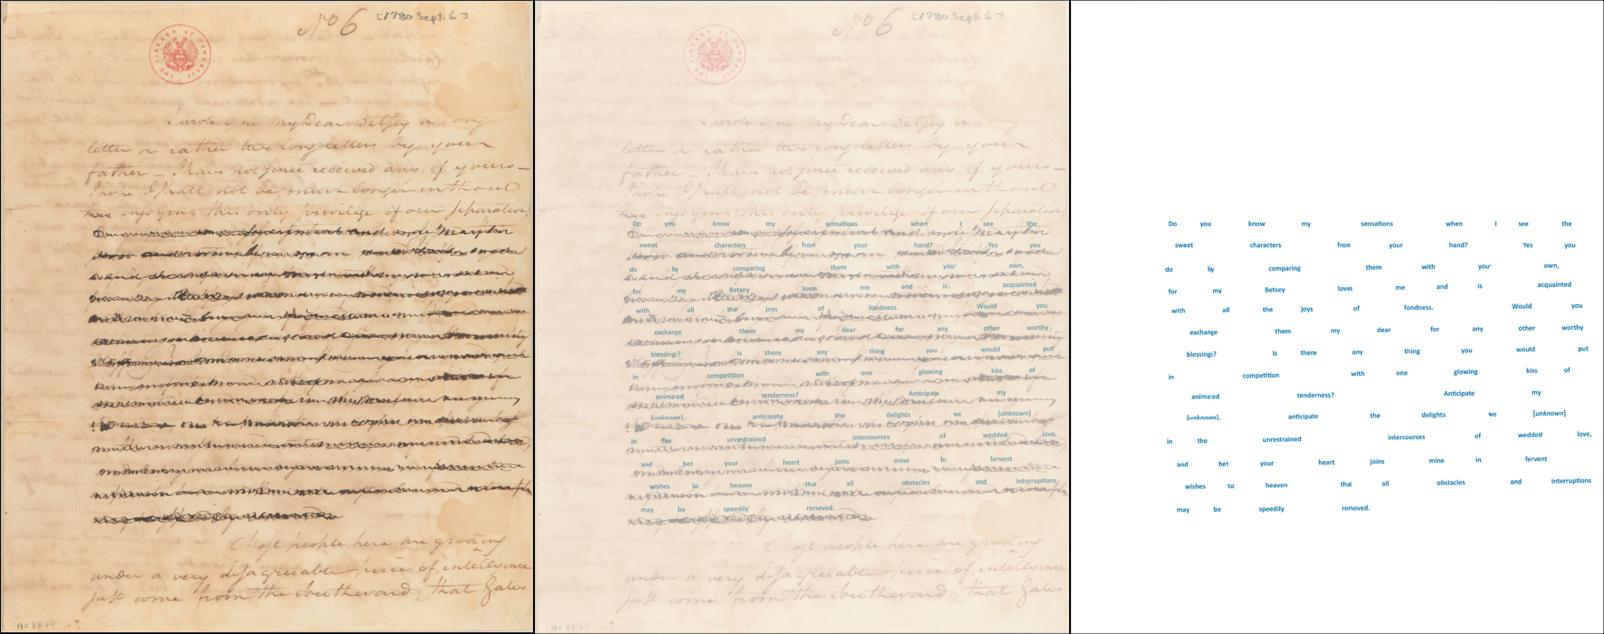
\includegraphics[width=\textwidth]{./textes/chap4/iiif-calque.jpg}
	\caption{Lettre d'Alexander Hamilton}
	\label{fig:info}
\end{figure}
Le projet de recherche \enquote{La couleur~: artefacts, matière et cognition} possède également des images numériques issues d’analyses hyperspectrales. Les laboratoires en charge des rapports d’analyses physico-chimiques ont fourni, au moment de leurs résultats, des doubles numériques au commanditaire. Il est ainsi possible d’envisager, à l’image de ce qu’a proposé la Bibliothèque du Congrès, de réaliser des claques sur les feuillets de manuscrit, permettant de découvrir les images hyperspectrales correspondantes et donc les résultats.\newpage

\section{La sélection du département des manuscrits}

Le fac-similé numérique produit est considérablement enrichi au regard de simples reproductions numériques d’images habituellement disponibles. Douze manuscrits ont fait l’objet d’une transformation en manifeste \indexmot{IIIF}\footnote{Les liens des manifestes \indexmot{IIIF} sont reportés en annexe.}. Ils sont retenus en raison de la qualité exceptionnelle de leurs enluminures. Une fois les sites Omeka~S accessibles au public, ils constitueront une petite sélection pour les utilisateurs, un modèle du travail effectué au cours des années du projet de recherche.\\\par
\begin{tabular}{>{\raggedright}p{0.5cm} >{\raggedright\arraybackslash}p{14cm}}
	1. & Le Psautier de Paris (BnF. Département des Manuscrits. Grec 139) \\[10pt]
	2. & L’Evangéliaire dit de Charlemagne ou de Godescalc (BnF. Département des Manuscrits. NAL 1203) \\[10pt]
	3. & Le Beatus a Liebana, Commentarius in Apocalypsin (BnF. Département des Manuscrits. Latin 8878) \\[10pt]
	4. & Les Evangiles dits d'Echternach ou de Saint Willibrord (BnF. Département des Manuscrits. Latin 9389) \\[10pt]
	5. & L’Ancien Testament et quelques feuillets du Nouveau Testament en syriaque (BnF. Département des Manuscrits. Syriaque 341) \\[10pt]
	6. & Le Tétraévangile (BnF. Département des Manuscrits. Copte 13) \\[10pt]
	7. & Les Makamat de Hariri (BnF. Département des Manuscrits. Arabe 5847) \\[10pt]
	8. & Le Codex Xolotl (BnF. Département des Manuscrits. Mexicain 1-10) \\[10pt]
	9. & L’Évangéliaire dit de Poussay (BnF. Département des Manuscrits. Latin 10514) \\[10pt]
	10. & Le Codex Sinopensis (BnF. Département des Manuscrits. Supplément Grec 1296) \\[10pt]
	11. & Le Psautier dit de saint Louis (BnF. Département des Manuscrits. Latin 10525) \\[10pt]
	12. & Un recueil d'œuvres en prose et en vers, probablement toutes dues à Naṣīr al-Dīn Muḥ. b. Ibrāhīm b. ʿAbd-ullāh al-Rammāl al-Muʿazzim al-Sāʿatī al-Haykalī (BnF. Département des Manuscrits. Persan 174) \\[10pt]
\end{tabular}

Les manuscrits sont tous enrichis de métadonnées descriptives. Ils offrent une première approche avec le manuscrit dans une courte introduction, puis quelques phrases qui retracent son historique, suit ensuite une petite fiche technique, puis un commentaire sur le texte et les images, une note sur le ou les artistes et, enfin, quelques grandes lignes sur les matériaux découverts lors des analyses. \par
Ci-dessous, l’exemple de la présentation du manuscrit Latin 10514 telle que visible dans Mirador~:\par

\begin{mdframed}[style=graybox]
	LIBELLÉ~:\par
	BnF. Département des Manuscrits. Latin 10514\par
	DESCRIPTION~:\par
	Évangéliaire dit de Poussay\par
	INTRODUCTION~:\par
	Réalisé dans l’abbaye de Reichenau à la fin du Xe siècle, vers 980, l’Évangéliaire de Poussay fait partie du groupe des manuscrits dit \enquote{de Ruodprecht}, d’après le copiste du Psautier d’Egbert, également originaire de Reichenau. Il s’agit d’un évangéliaire festif contenant des enluminures sur fond pourpre. Sa destination est incertaine, mais il a été offert vers 1036 à l’abbaye de Poussay par Brunon d’Eguisheim-Dagsbourg, alors évêque de Toul et devenu pape entre 1049-1054 sous le nom de Léon~IX.\par
	POSSESSEURS~:\par
	Trésor de l’abbaye de Poussay jusqu’à la Révolution française (?)~; bibliothèque de la Ville de Mirecourt~; acquis en 1844 par la Bibliothèque royale contre des livres imprimés.\par
	DESCRIPTION TECHNIQUE~:\par
	285 x 205 mm 133 feuillets de parchemin\par
	TEXTES ET IMAGES~:\par
	13 peintures en pleine page~: f.~3v Ecclésiastique offrant son livre, conduit par 2 anges~; f.~4r Christ trônant, main étendue vers le donateur~; f.~5v saint Luc inspiré par le bœuf~; f.~6r saint Marc inspiré par le lion~; f.~7v saint Jean examinant sa plume~; f.~8r saint Matthieu écrivant~; f.~9v Nativité~; f.~18v Adoration des mages~; f.~35v crucifixion~; f.~46v le lavement des pieds~; f.~50v deux saintes femmes au Tombeau~; f.~66v Ascension~; f.~69v Pentecôte~; 16 pages d’initia ornées~: f.~10r~; f.~13r~; f.~19r~; f.~25r~; f.~36r~; f.~49r~; f.~51r~; f.~67r; f.~70r~; f.~81r~; f.~84r~; f.~95r~; f.~97r~; f.~102r~; f.~119r~; 7~pages d’incipit ornées~: f.~12v~; f.~48v~; f.~80v~; f.~94v ~; f.~96v~; f.~101v~; f.~118v.\par
	ARTISTES~:\par
	Le décor est de la main d’un seul artiste, dont le style se caractérise par la monumentalité des personnages représentés et la densité de certaines compositions. Son style a été rapproché de celui du Psautier d’Egbert (Cividale, Museo Archaeologico Nazionale, cod. 136) qui fut évêque de Trèves à partir de 977.\par
	MATÉRIAUX~:\par
	Les fonds des enluminures à pleines pages sont pourprés. La palette utilisée est large mais délimitée~: rouge, vert, jaune, doré, violet, des touches de bleus et des nuances de bruns et de gris. Le bleu est réalisé à partir d’outremer (lapis-lazuli)~; les tons de rouge, de violet et parfois de brun contiennent de l’orseille, pigment obtenu à partir de lichen, mélangé parfois avec de l’oxyde de plomb pour le marron. Le jaune contient de l’ocre jaune, qui est associé au vert-de-cuivre pour obtenir les teintes de couleur verte.\\\par
\end{mdframed}

En deuxième lieu, les manifestes sont annotés selon les points d’analyses qui sont renseignés dans les données de la base. Il faut faire un choix pour le commentaire des annotations, trois informations sont retenues~: le motif analysé, la couleur et les matériaux découvert. Ces trois données sont celles qui correspondent le mieux au principe de l’annotation, puisqu’elles concernent des points d’analyses précis, là où d’autres concernent le feuillet ou le manuscrit. Si je reprends le cas du manuscrit Latin 9389, les informations de la base sont reportées selon le modèle ci-dessous, à gauche. Seuls les commentaires du Latin 8878 ont une autre présentation, comme visible à droite.\par
\begin{figure}[H]
	\centering
	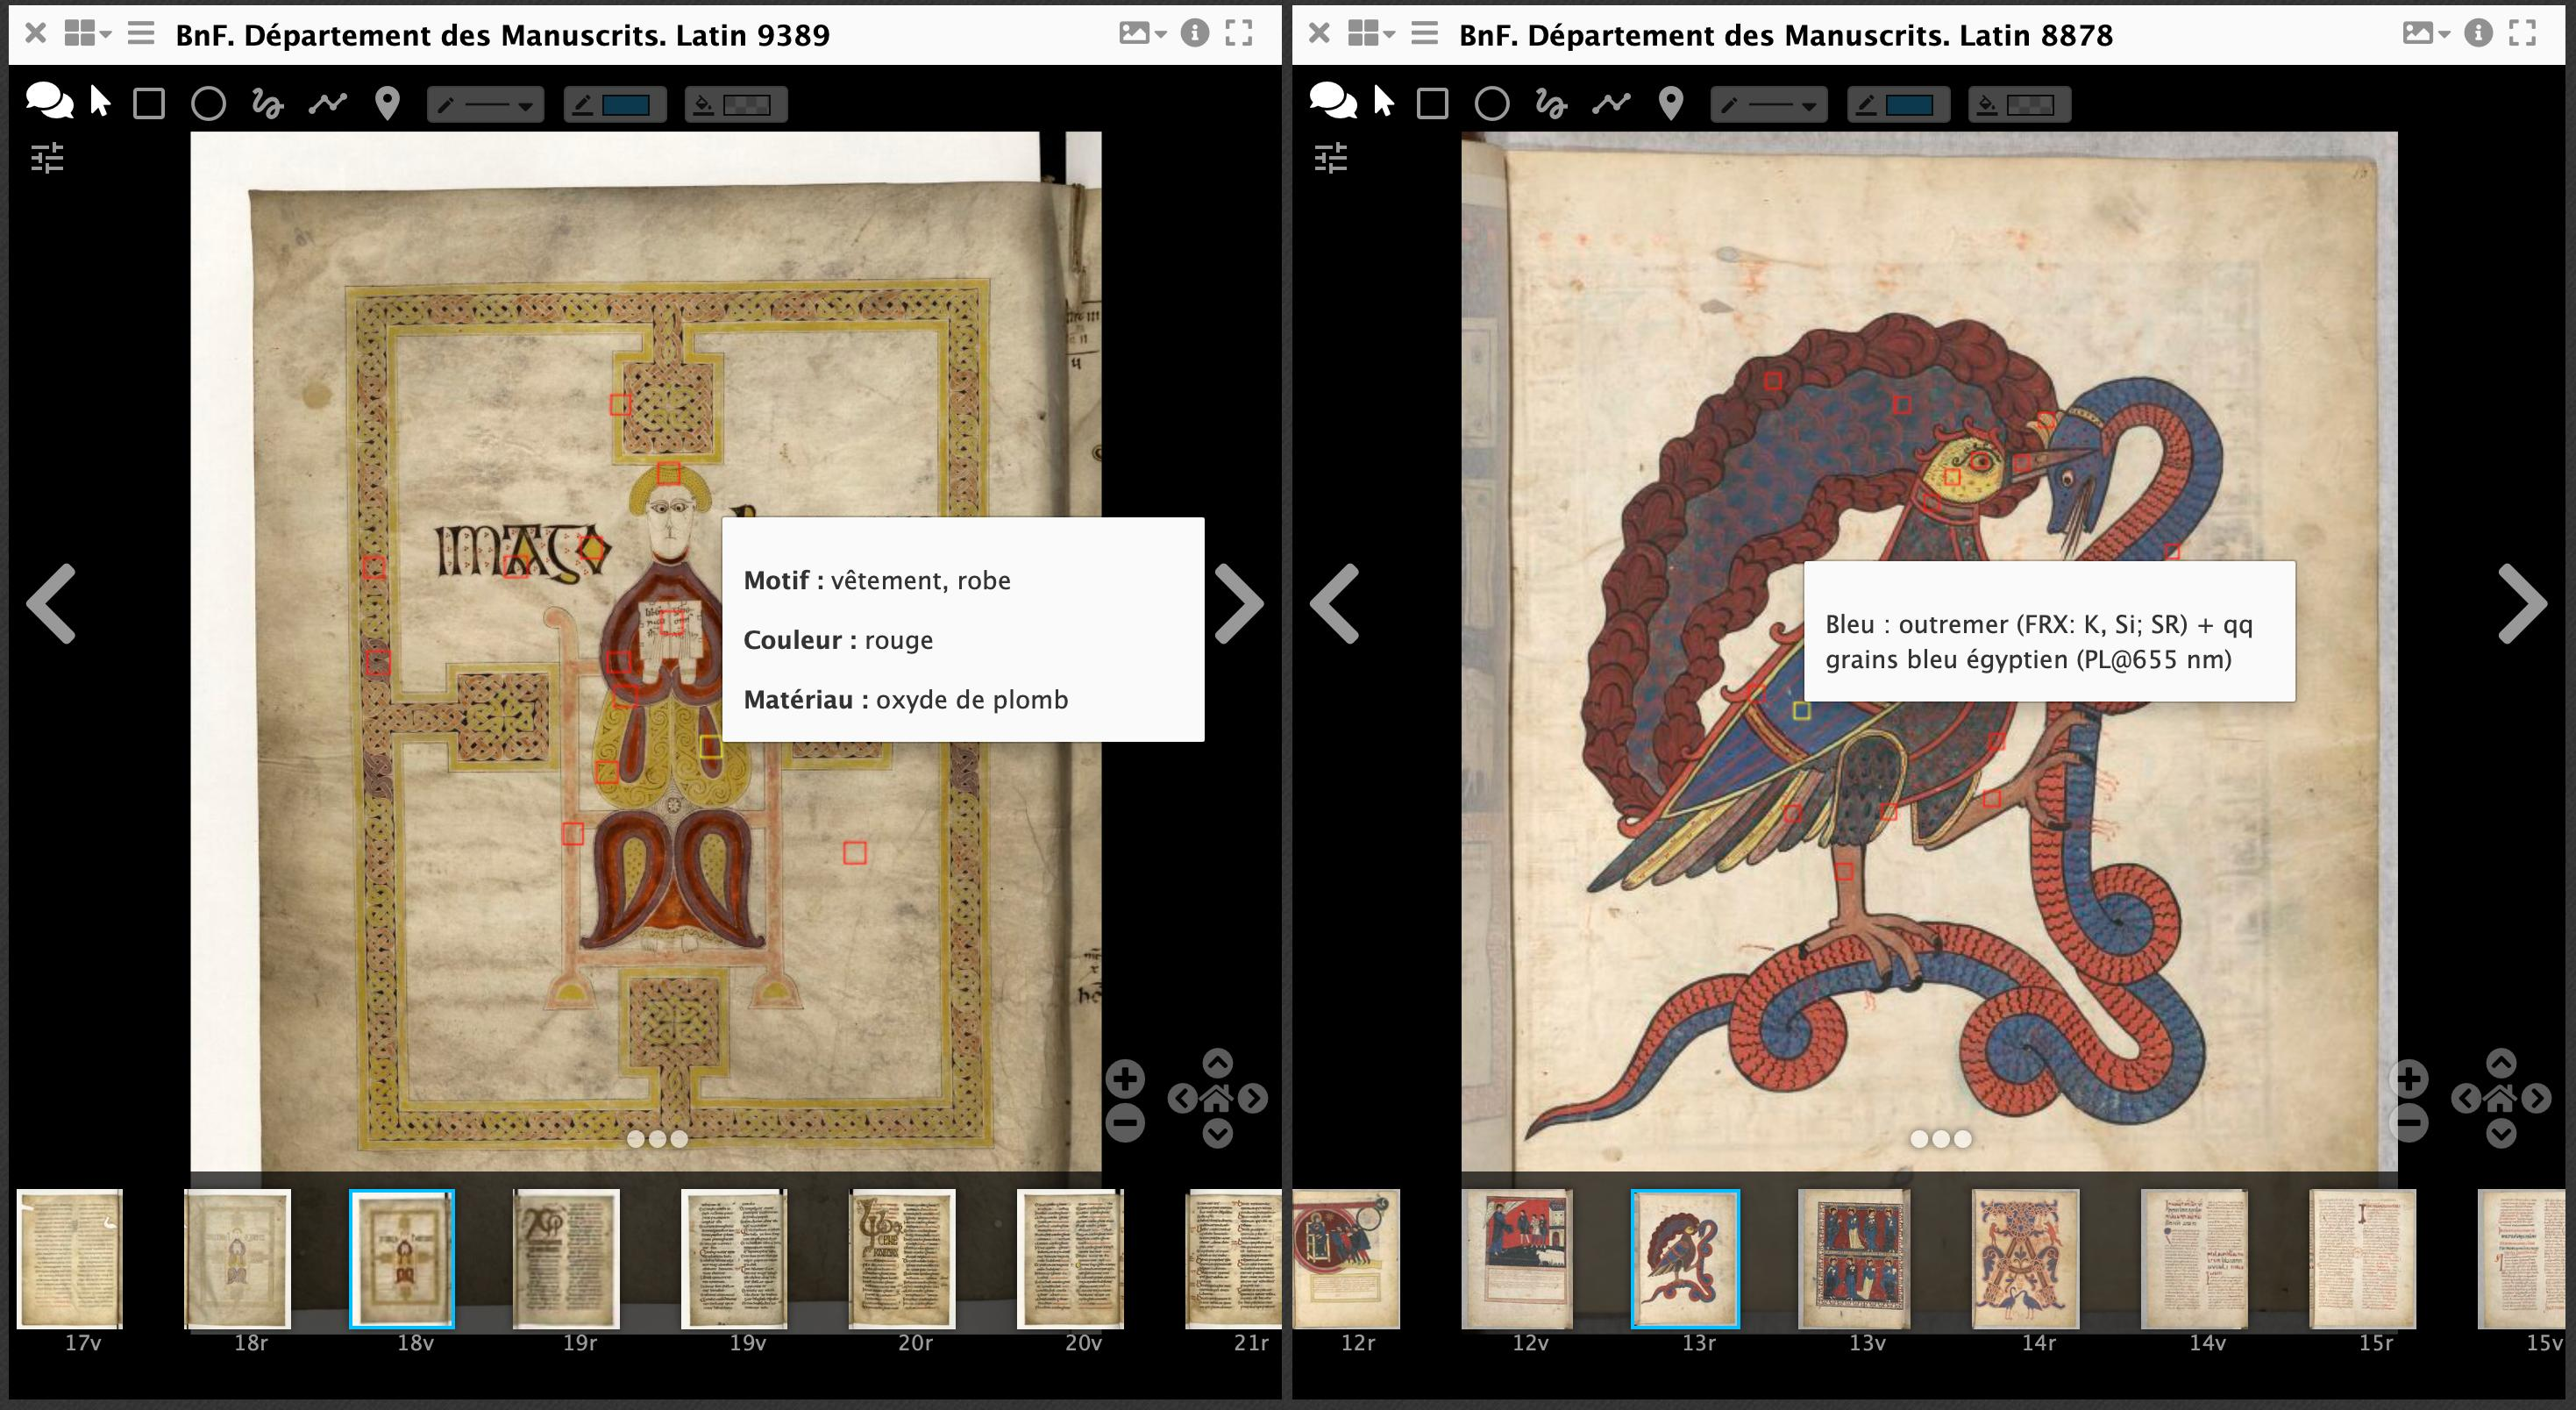
\includegraphics[width=\textwidth]{./textes/chap4/iiif-annot.jpg}
	\caption{Annotations dans Mirador}
	\label{fig:info}
\end{figure}
Enfin, un système de calque vient mettre en complément de l’image numérique du feuillet les résultats obtenus par les analyses hyperspectrales. Ils sont invisibles au chargement de la page, mais ils apparaissent une fois sélectionnés dans la barre latérale. L’affichage sous Mirador permet de cumuler l’affichage des calques à celles des annotations. Ainsi, il est permis d’additionner les résultats de différentes analyses pour avoir toutes les informations nécessaires sur le feuillet en question.\par
\begin{figure}[H]
	\centering
	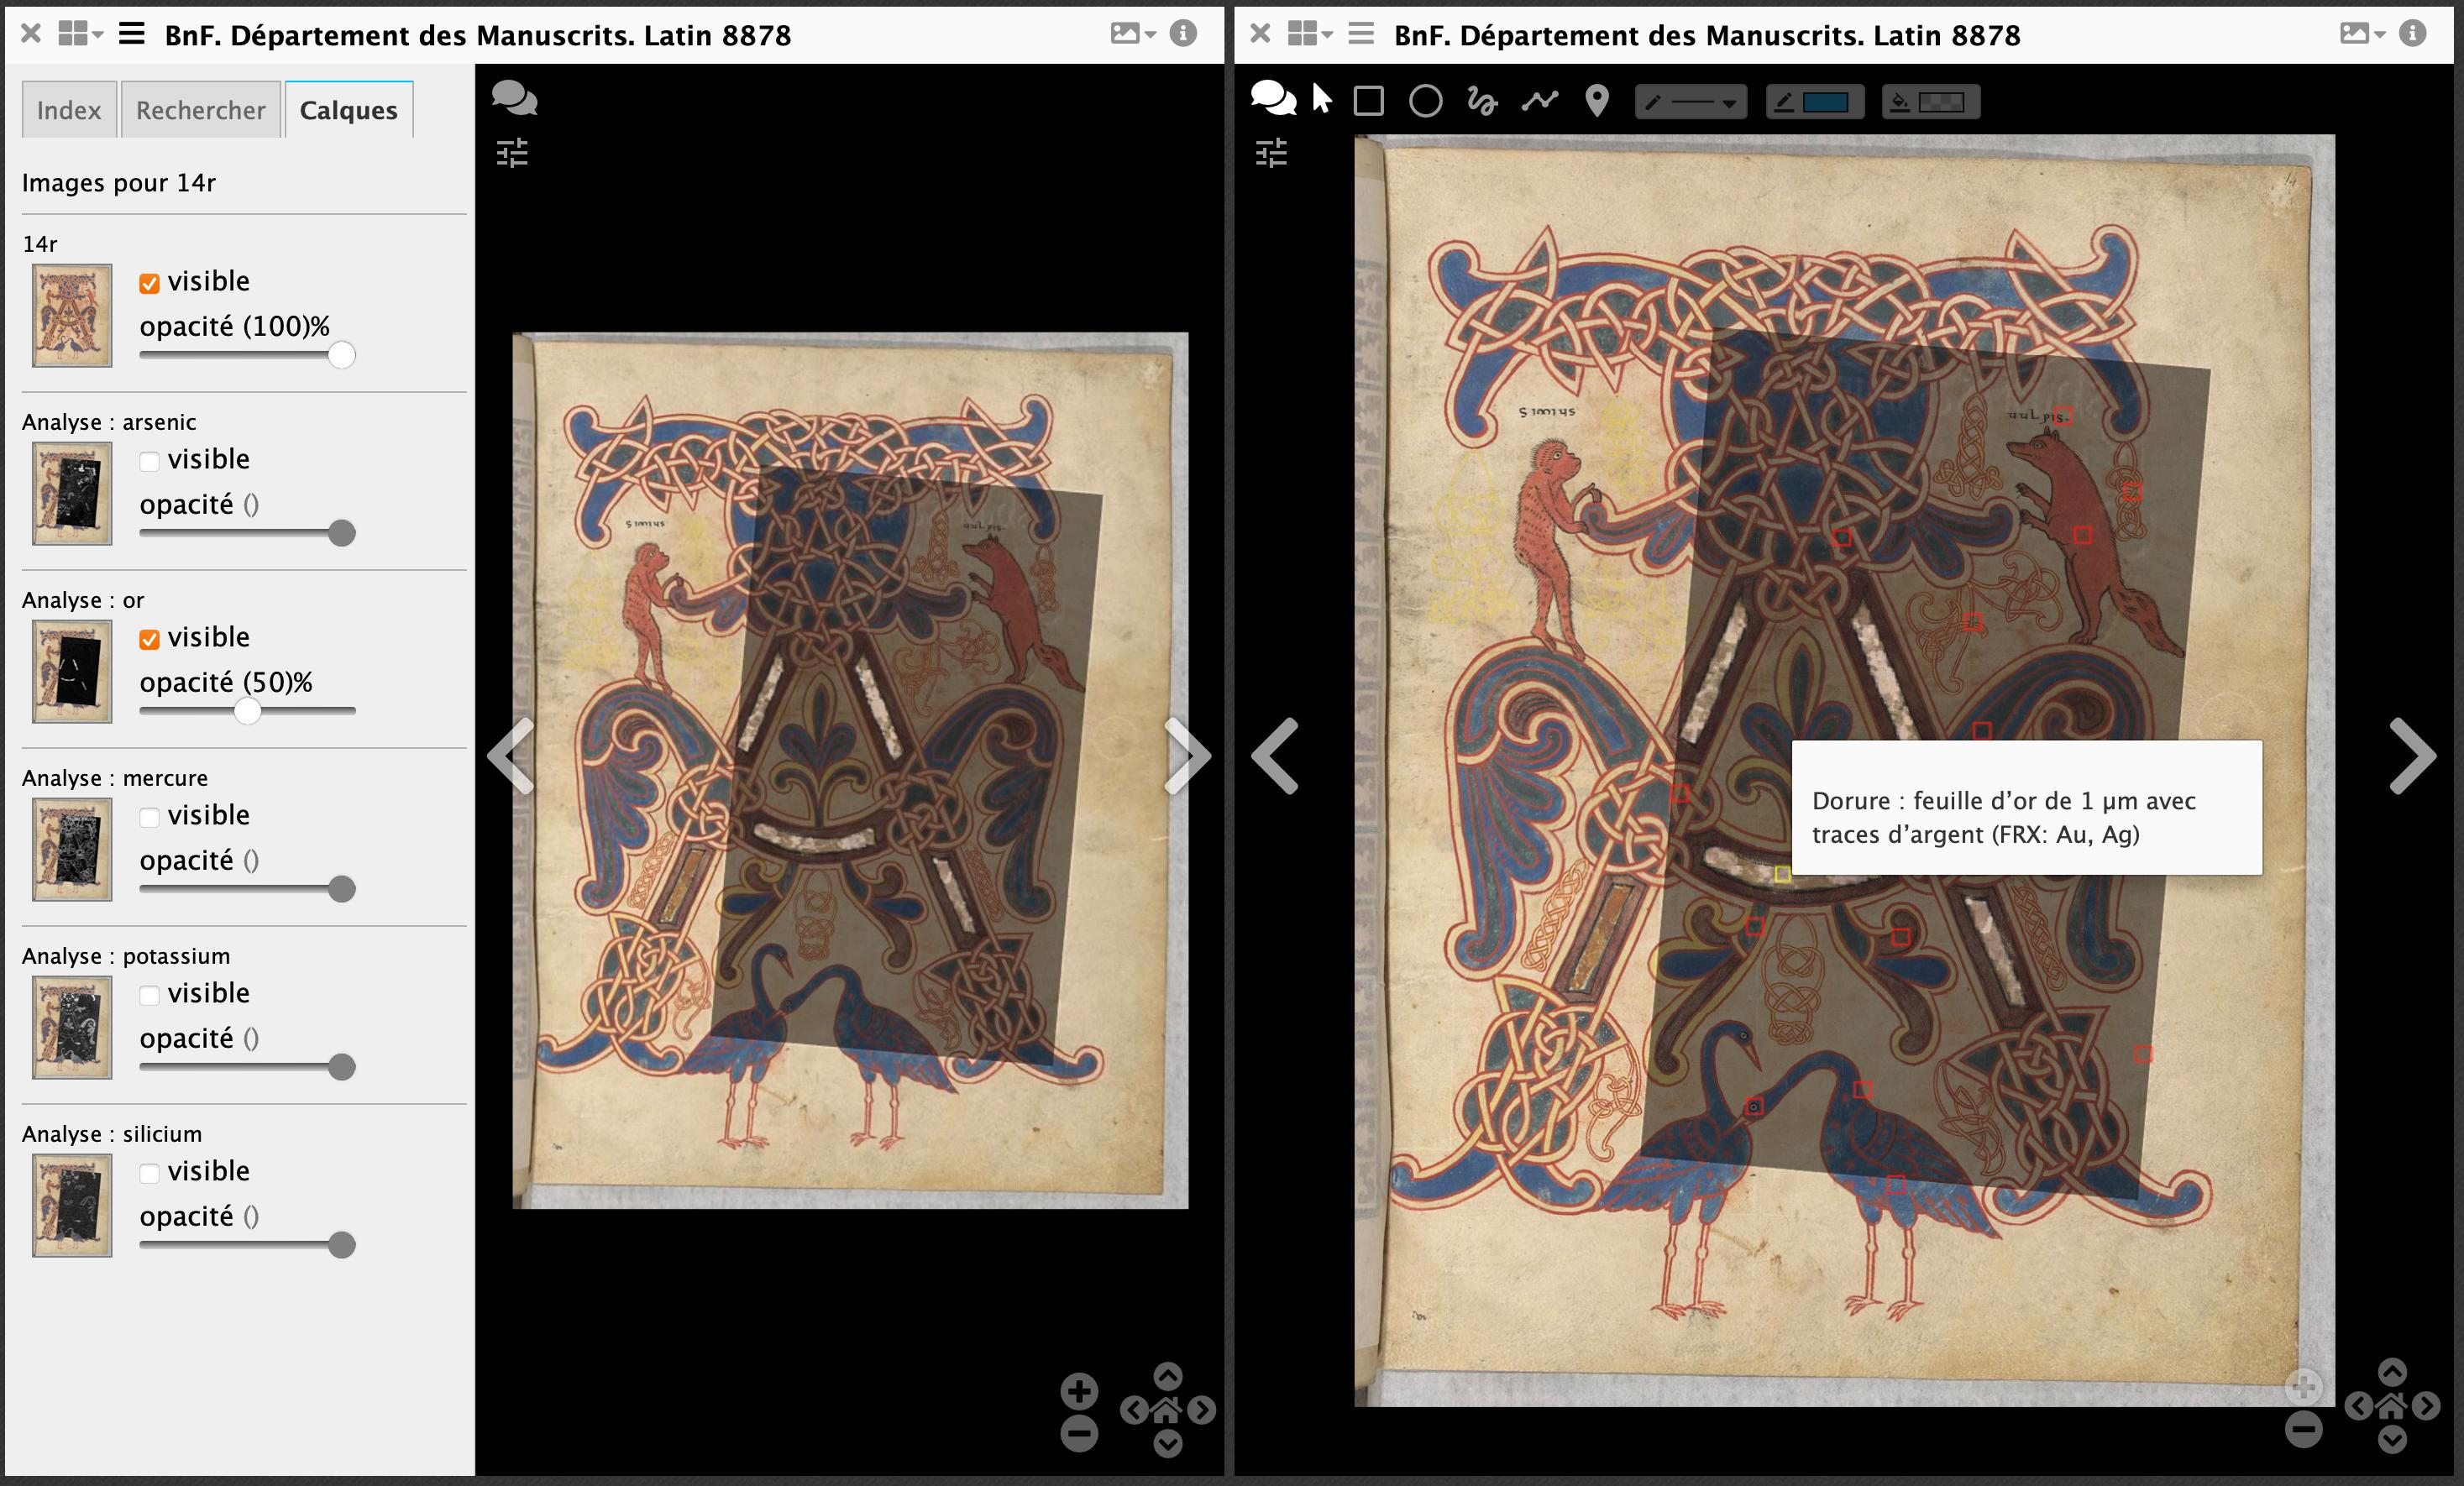
\includegraphics[width=\textwidth]{./textes/chap4/iiif-calque-annot.jpg}
	\caption{Addition d'un calque et d'une annotation}
	\label{fig:info}
\end{figure}
Un fac-similé de cette nature facilite la communication et la médiation de la recherche. Les chercheurs ont à leur disposition les images numériques en haute résolution des feuillets, la présentation du manuscrit, ainsi que le résultat des analyses menées dans le cadre du projet de recherche. Les données de la base sont à la disposition du public, mais elles sont également intelligibles parce que contextualisées sur la source même du travail. Elles ne sont plus inscrites dans des CSV à plusieurs milliers de lignes, mais sur l’objet même de la recherche. \par
Le fac-similé numérique permet aussi d’instaurer un langage commun entre des cultures scientifiques diverses. Ainsi, le scientifique et les historiens, historiens de l’art, spécialistes des textes anciens ont sous les yeux le document qui est l’objet de leur discussion. Ils peuvent y rapporter directement leurs commentaires, leurs analyses et leurs résultats. Des étapes de traductions scientifiques, qui peuvent être parfois à la source d’erreurs, non plus lieu d’être et les processus de communication sont simplifiés.\newpage

*\\\par
Le projet détaillé ici n’a pu trouver son aboutissement dans le cadre de ce stage. Les deux projets scientifiques sont hébergés à partir de l’automne sur un site Omeka~S. En conséquence, et en anticipation de la migration, un essai d’implémentation d’une visionneuse dans Omeka~S\footnote{Pour l’implémentation de Mirador dans Omeka S, voir annexe 3.} a été réalisé. Cet essai a également pour objectif de s’assurer de la bonne conformité des manifestes~\indexmot{IIIF} précédemment cités. Cependant, il s’est avéré que le module Mirador proposé pour Omeka est appauvri par rapport aux versions de la visionneuse qui peuvent être trouvées sur le web. Si une solution a été trouvée pour la gestion des annotations, il n’en est pas de même pour les calques d’images\footnote{Cf annexe 4.}. Les manifestes qui seront proposés à l’automne sur les sites Omeka~S ne proposeront donc pas ce dernier enrichissement pour les fac-similés. Néanmoins, les facs-similés numériques produits demeurent de nouveaux outils de recherche mis à la disposition du public et utiles pour la communication de la recherche. 
	\cleardoublepage
		
	\chapter*{Conclusion}
	\addcontentsline{toc}{chapter}{Conclusion}
	\markboth{\small\textit{Conclusion}}{}
	Les programmes de recherche sur \enquote{La couleur~: artefacts, matière et cognition} et sur \enquote{La fabrique matérielle du visuel~: panneaux peints en Méditerranée} ont abouti à trois projets de \indexmot{visualisation}~: une \indexmot{carte interactive}, une \indexmot{frise chronologique} et une édition de fac-similés numériques. Ces \indexmot{visualisation}s prolongent et enrichissent les recherches des années précédentes. Elles permettent de réexaminer les données collectées et les résultats obtenus, elles facilitent la communication et la médiation de la recherche, et elles instaurent un langage commun entre diverses cultures scientifiques. Ainsi, une politique de \indexmot{visualisation} des données doit être intégrée dans la réflexion du chercheur dès le lancement d’un programme de recherche.\\\par
Ce mémoire a démontré que les \indexmot{visualisation}s ne sont pas simplement des outils à disposition du chercheur, mais qu'elles produisent et reflètent également des connaissances historiques. La cartographie interactive et la \indexmot{frise chronologique} proposent ainsi une mise en ordre du temps et de l’espace selon l’histoire des enluminures des manuscrits et des panneaux peints. Chaque réalisation est située par rapport aux autres, en fonction d’un système de repérage constitué de coordonnées ou de dates. Il s’agit de représenter, de distinguer ou de regrouper une réalisation par rapport à une autre, selon leur contexte géographique ou temporel.\par
Ces \indexmot{visualisation}s sont à l’origine d’un discours sur l’espace et sur le temps pour le chercheur. Elles permettent d’identifier des tendances historiques et des contextes de production, autrement dit des alignements de données, qui doivent être explorés. Le chercheur, parfois submergé par les milliers de lignes d’un fichier~CSV, peut perdre de vue l’ensemble des données. Les \indexmot{visualisation}s redonnent un sens aux analyses produites, les orientant selon des préoccupations chronologiques et géographiques. Elles permettent également de faire ressortir les données essentielles et de reléguer les autres à leur place accessoire ou complémentaire, grâce à des politiques d’éditorialisation de la base, qui, comme nous l’avons vu, est avant tout un encodage de filtres sur les \indexmot{thésaurus} constitués.\par
Les fac-similés numériques, troisième et dernier volet des \indexmot{visualisation}s, facilitent la communication et la médiation de la recherche. Les données de la base sont reportées sur des images numériques en haute résolution avec des métadonnées de présentation. Les analyses menées, qui constituent le travail scientifique des chercheurs lors du projet de recherche, deviennent intelligibles au public parce que contextualisées sur la source même du travail. Le fac-similé numérique permet aussi d’instaurer un langage commun entre des cultures scientifiques diverses. Ainsi, le scientifique et les historiens, historiens de l’art, spécialistes des textes anciens ont sous les yeux le document qui est l’objet de leur discussion. Ils peuvent y rapporter directement leurs commentaires, leurs analyses et leurs résultats. Des étapes de traduction scientifique, qui peuvent parfois être à la source d’erreurs, n'ont plus lieu d’être et les processus de communication sont simplifiés.\\\par
Ce mémoire fait apparaître que la \indexmot{visualisation} n’est plus seulement la représentation de l’analyse d’un chercheur avec des outils informatiques. Dans un certain sens, une logique s’inverse~: la \indexmot{visualisation} n’est plus une fin, mais tend à devenir un moyen, une étape de la recherche. Avec cette redéfinition, le public de la \indexmot{visualisation} change aussi. Elle ne se réduit plus au grand public, à des fins de communication de la recherche, mais elle devient un service de la recherche, désormais en soutien aux chercheurs.\par
Cette évolution conduit à repenser les différentes séquences des projets de recherche. D’un schéma en trois temps, où se succèdent \enquote{recherche}, \enquote{analyse} et \enquote{publication (dont \indexmot{visualisation})}~; il conviendrait de passer à une nouvelle articulation \enquote{recherche}, \enquote{traitement informatique (dont \indexmot{visualisation}) et analyse}, puis \enquote{publication}. La réunion de l’analyse et du traitement informatique est déjà une réalité dans les projets de recherche actuels et ne cesse de se renforcer, en témoigne la place croissante prise par les ingénieurs d’étude et de recherche à côté des chercheurs dans le monde de la recherche.
	\newpage{\pagestyle{empty}\cleardoublepage}
	
	%%%%%%%%%%%%%%%%%%
	\appendix
	
	\chapter[Analyse du Beatus]{Analyse du combat du paon et du serpent dans le Beatus de Saint-Sever}
	\begin{figure}[H]
	\centering
	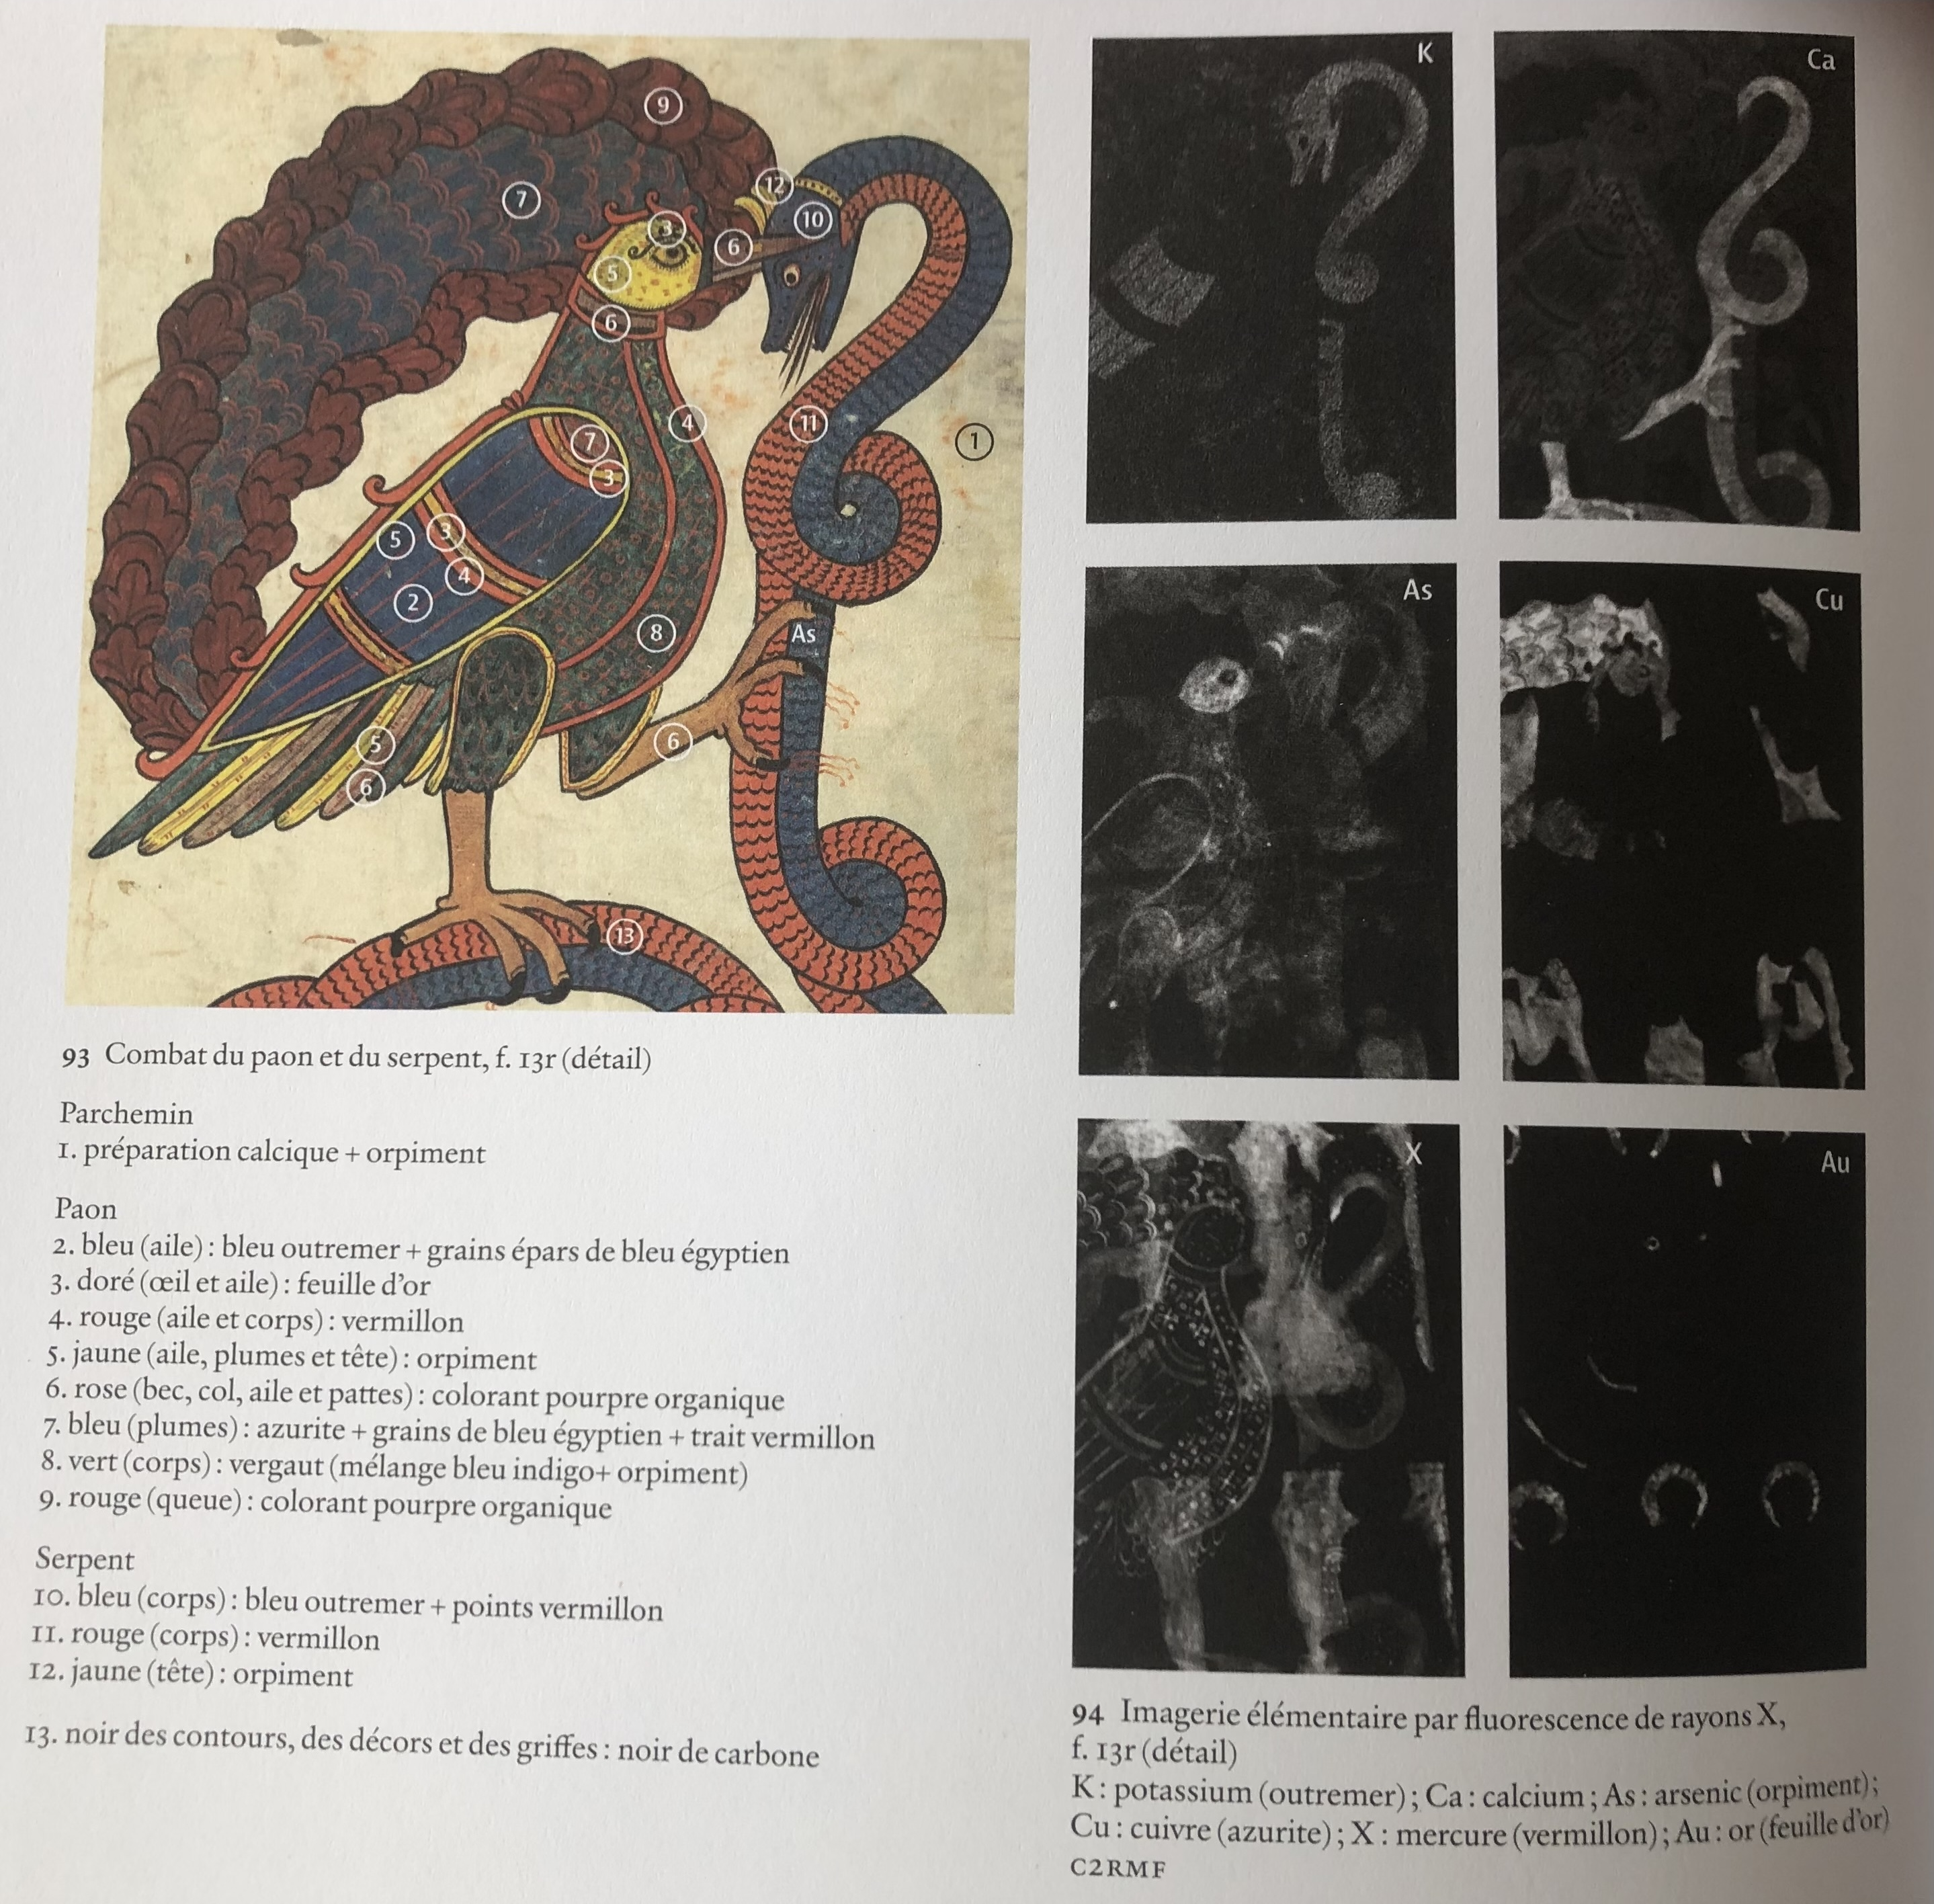
\includegraphics[scale=0.15]{./textes/annexe/analyse-beatus.jpeg}
	\label{fig:info}
\end{figure}
	\chapter[Analyse en JSON]{Exemple d’analyse de feuillet en JSON}
	\begin{lstlisting}[language=json]
	{
		"geometry": {
			"type": "Point",
			"coordinates": [
			6.95,
			50.93333
			]
		},
		"properties": {
			"Titre": "Sacramentaire de Saint-Géréon de Cologne, Monogramme VD avec la Croix, Paris, BNF, ms. Latin 817, f. 14v",
			"Parent": "02389266-ee27-48ea-be1e-0b40e5e0144e",
			"Type": "manuscrit – sacramentaire – enluminure",
			"Attribution": "?",
			"Lieu_de_creation": "Cologne – Allemagne",
			"Realisation": "1051 – 1000",
			"Identifiant": "02389266-ee27-48ea-be1e-0b40e5e0144e_001",
			"Image": "https://agorha.inha.fr/ark:/54721/ce34ce88-1066-452d-8732-1640d085e348/doc/802fb768-aec9-4d2f-a45a-c409bb9dab1b/original.PNG",
			"Type_description": "Couche colorée",
			"Caracteristique": "Couche picturale",
			"Motif": "décor",
			"Technique": "enluminé – gouache",
			"Couleur": "rouge – rouge foncé",
			"Materiaux": "orseille",
			"Certitude": "supposé",
			"Technologie": "FORS – XRF",
			"Mesure": "?",
			"Date": "2023",
			"Rapport": "?",
			"Source": "?",
			"Localisation": "BnF - département des Manuscrits",
			"Cote": "Latin 817",
			"Date_filtre": "1051",
			"Projet": "La fabrique de l'art. Couleurs et matériaux de l'enluminure"
		},
		"type": "Feature"
	}
\end{lstlisting}
	\chapter[Mirador dans Omeka ~S]{Mirador dans Omeka~S}
	Une visionneuse, comme Mirador, s’implémente par un module propre à Omeka. Plus qu’un module, il convient plus précisément d’en télécharger trois pour que la visionneuse soit en capacité d’afficher convenablement un manifeste IIIF~:
\begin{itemize}
	\item \texttt{le module Common\footnote{https://gitlab.com/Daniel-KM/Omeka-S-module-Common}}~: qui permet de gérer les fonctionnalités internes utilisées dans divers modules (fonctions en bloc, éléments de formulaire, assistants de vue, tâches uniques pour l'installation et les paramètres, etc.), de sorte qu'il évite au développeur de copier-coller du code commun entre les modules.\par
	\item \texttt{le module IIIF Server\footnote{https://gitlab.com/Daniel-KM/Omeka-S-module-IiifServer}}~: qui intègre les spécifications IIIF pour permettre de traiter et de partager instantanément des images de toute taille et de tout support (pdf, audio, vidéo, 3D...) dans les formats souhaités.\par
	\item \texttt{le module Mirador\footnote{https://gitlab.com/Daniel-KM/Omeka-S-module-Mirador}~:} une visionneuse en ligne avancée, qui affiche des images, des livres, des cartes, etc. via la norme IIIF. La visionneuse est multi-fenêtres, avec la possibilité de zoomer, d'afficher, de comparer et d'annoter des images.
\end{itemize}\par

Les deux derniers modules doivent être paramétrés pour qu’ils puissent lire un manifeste tiers. Il faut, pour ce faire, définir pour propriété du \enquote{Dublin Core~: A un format}.\par
\begin{figure}[H]
	\centering
	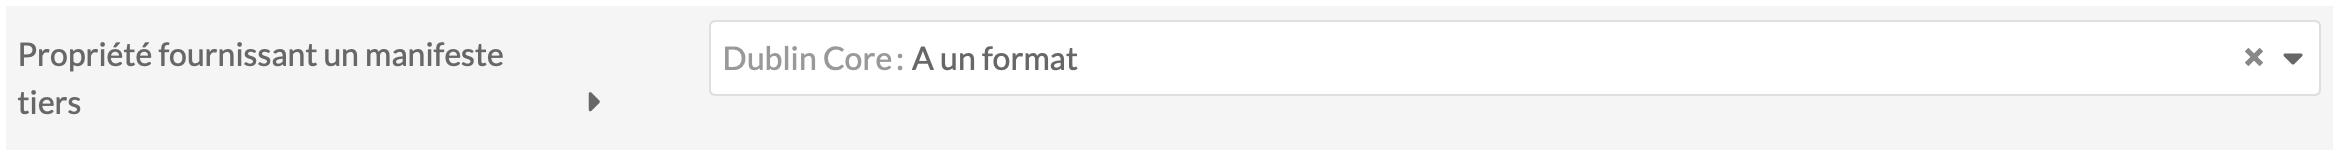
\includegraphics[width=\textwidth]{./textes/annexe/omeka-format.jpg}
	\label{fig:info}
\end{figure}

Pour ajouter un manifeste à une collection sur Omeka, il faut se rendre dans l’onglet \enquote{ressources}, \enquote{contenus}, puis \enquote{ajouter un contenu}.\par Ensuite, tout se fait dans l’onglet \enquote{valeurs}. Après avoir attribué un titre à l’objet, il convient de rechercher la propriété \enquote{a un format} de Dublin Core pour ajouter le manifeste.\par

\begin{figure}[H]
	\centering
	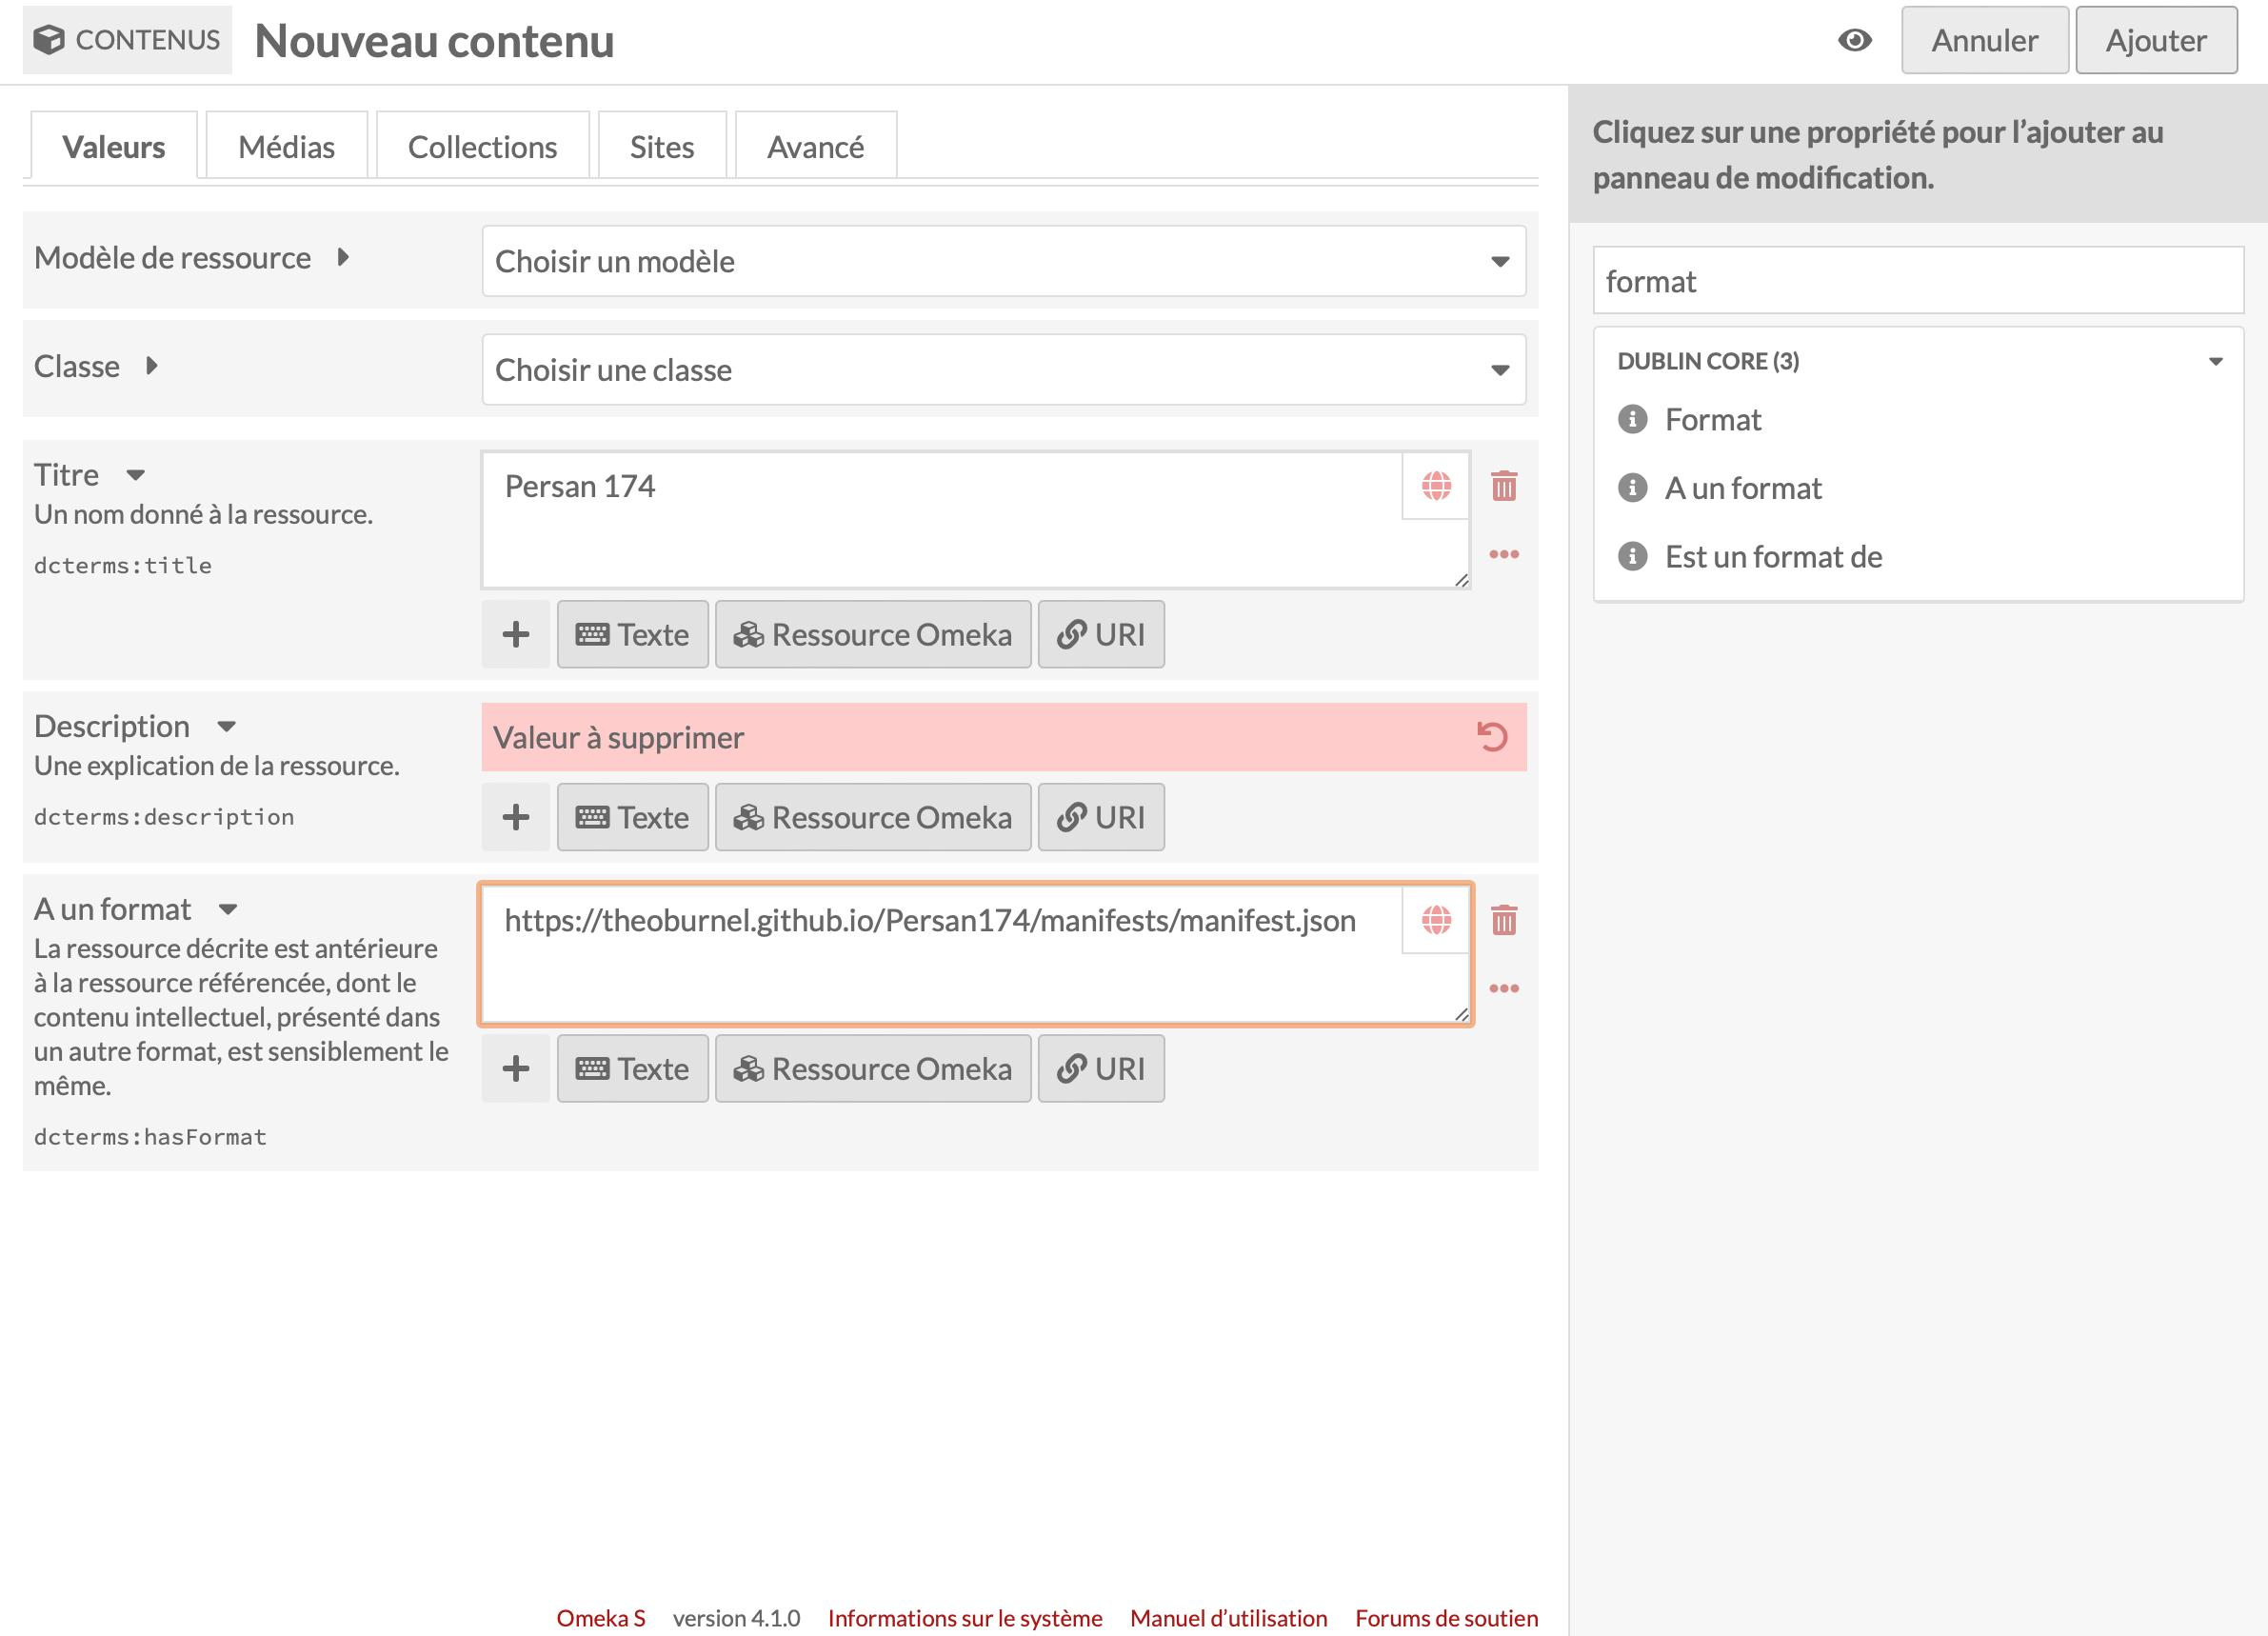
\includegraphics[scale=0.15]{./textes/annexe/omeka-item.jpg}
	\label{fig:info}
\end{figure}

Pour faire apparaître le manifeste IIIF sur la page internet, il suffit d’ajouter un bloc \enquote{Mirador Viewer} et de mettre comme pièce jointe le manifeste souhaité. Après l’enregistrement, le manifeste et les annotations apparaissent.\par

\begin{figure}[H]
	\centering
	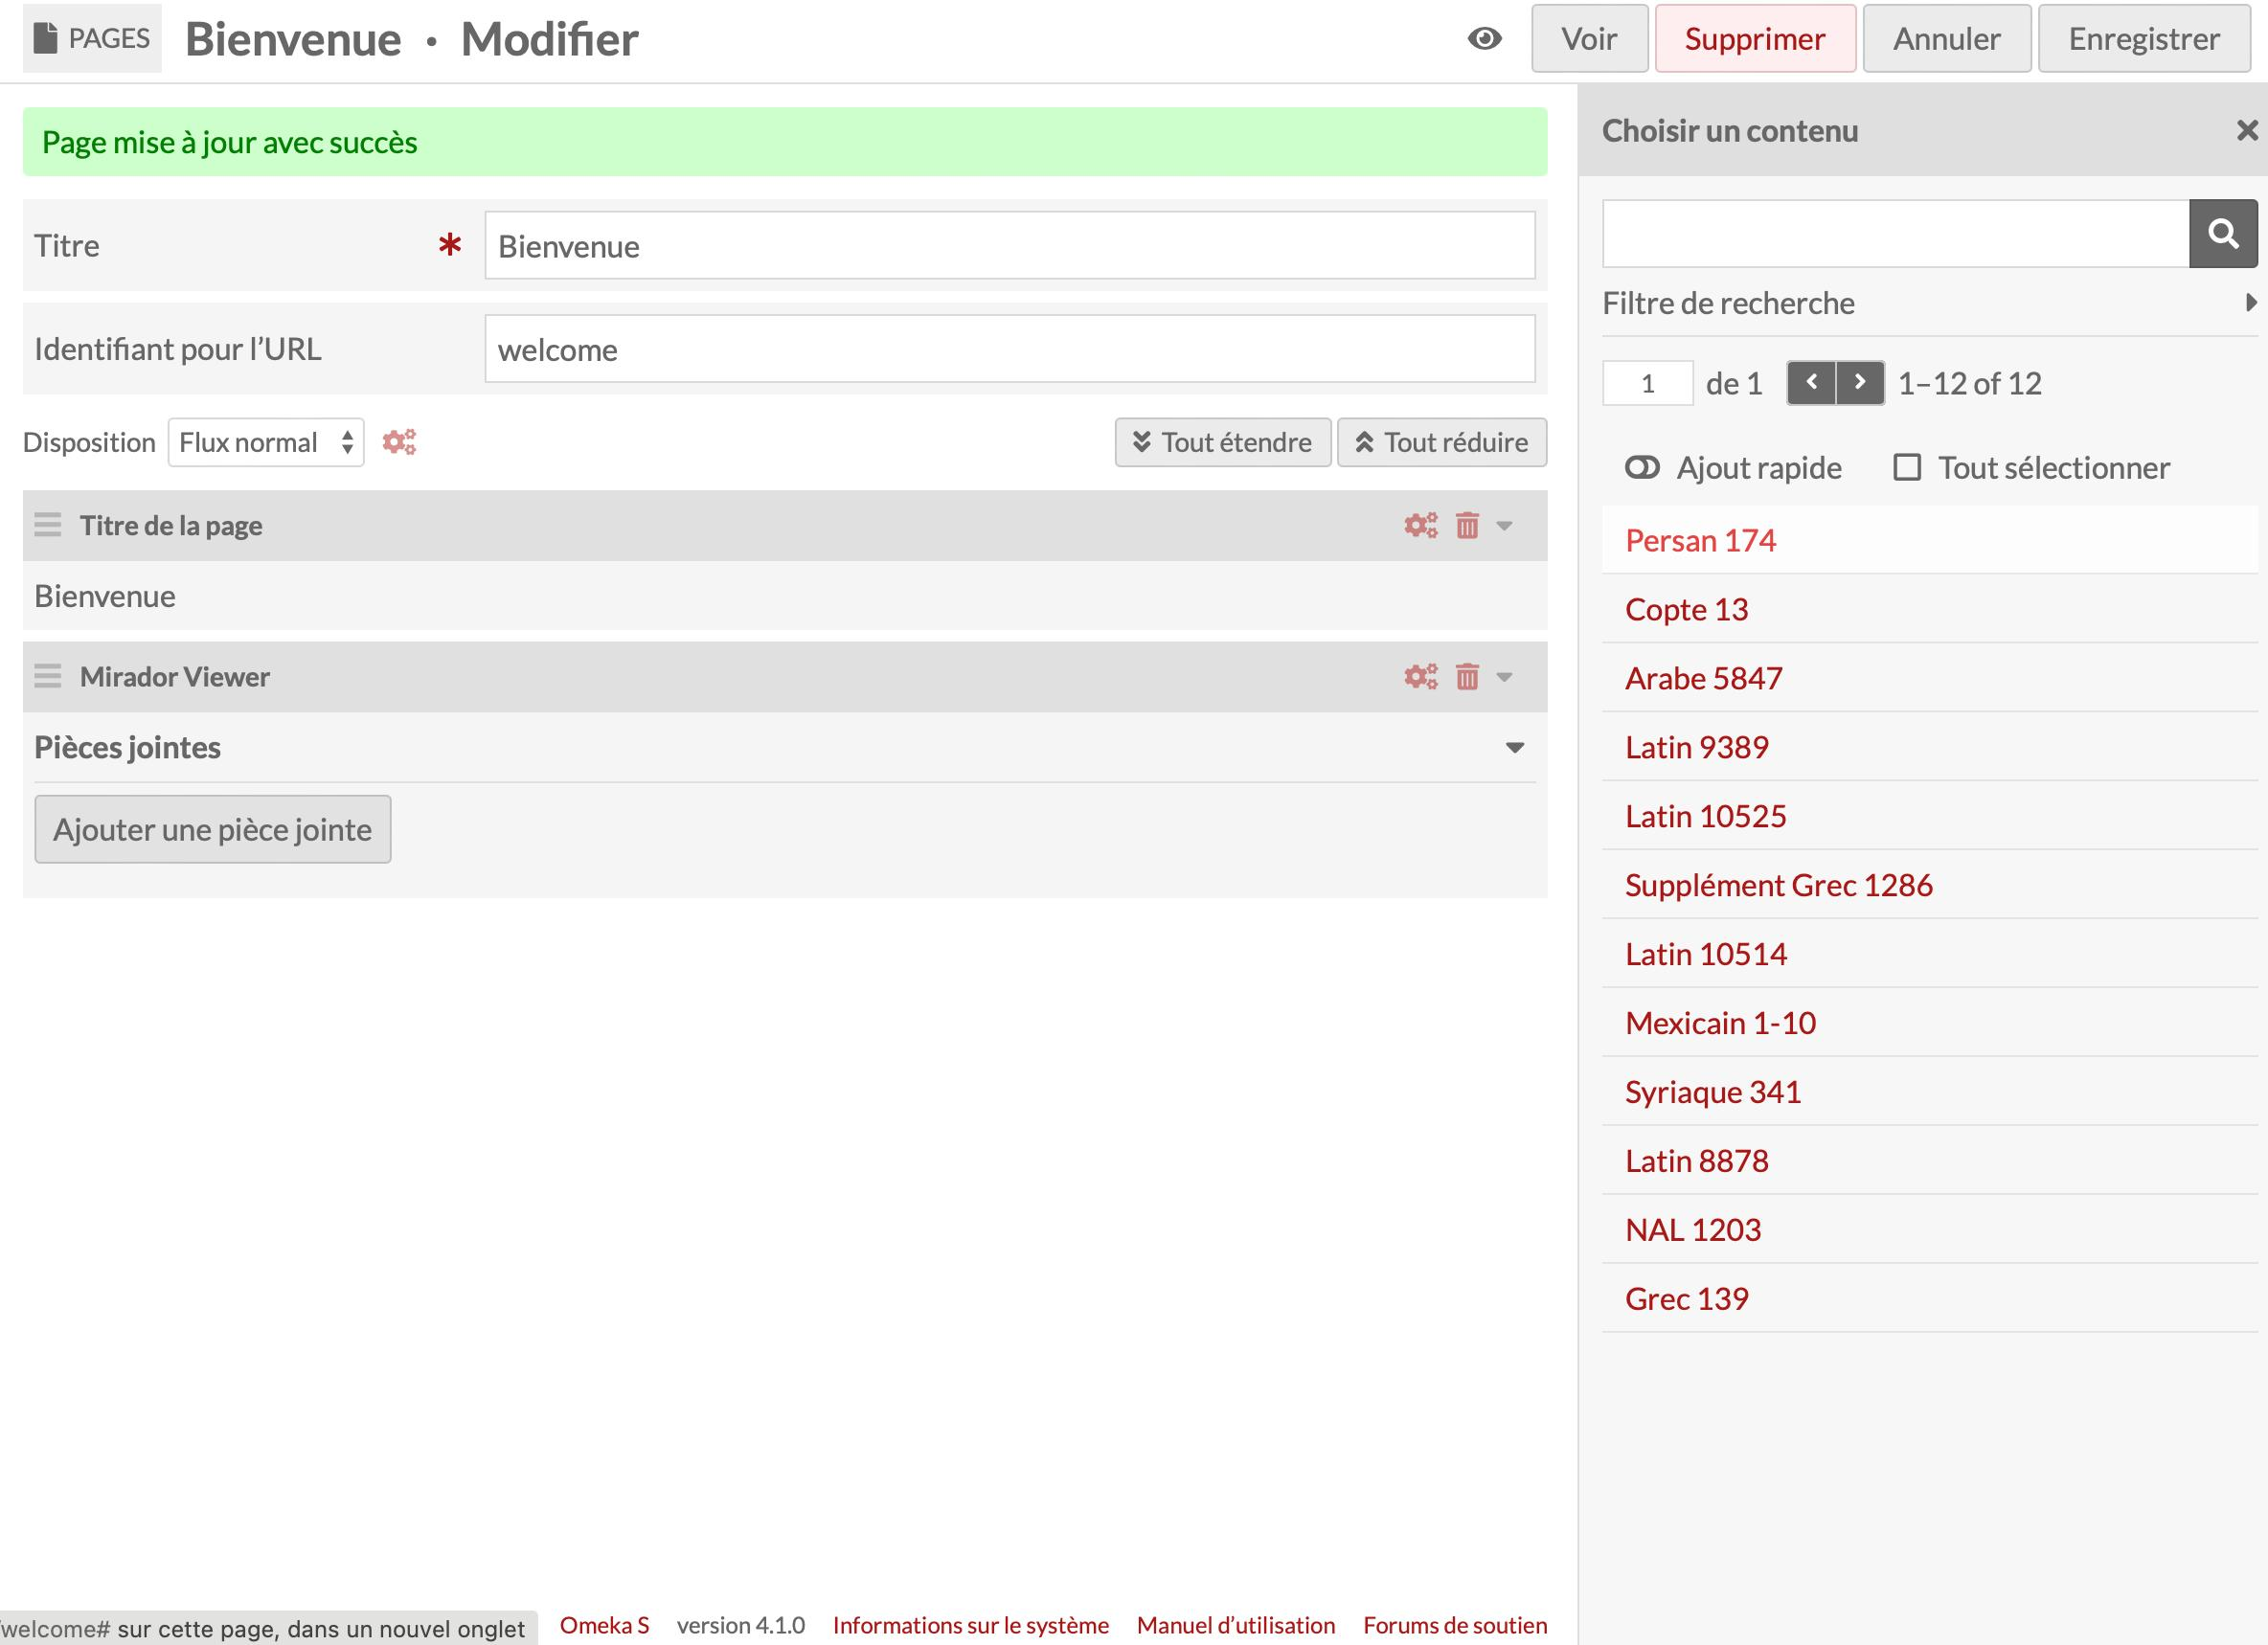
\includegraphics[scale=0.15]{./textes/annexe/omeka-visu.jpg}
	\label{fig:info}
\end{figure}

Ci-dessous, un exemple d’une visualisation d’une image IIIF sur Omeka S avec la visionneuse Mirador.

\begin{figure}[H]
	\centering
	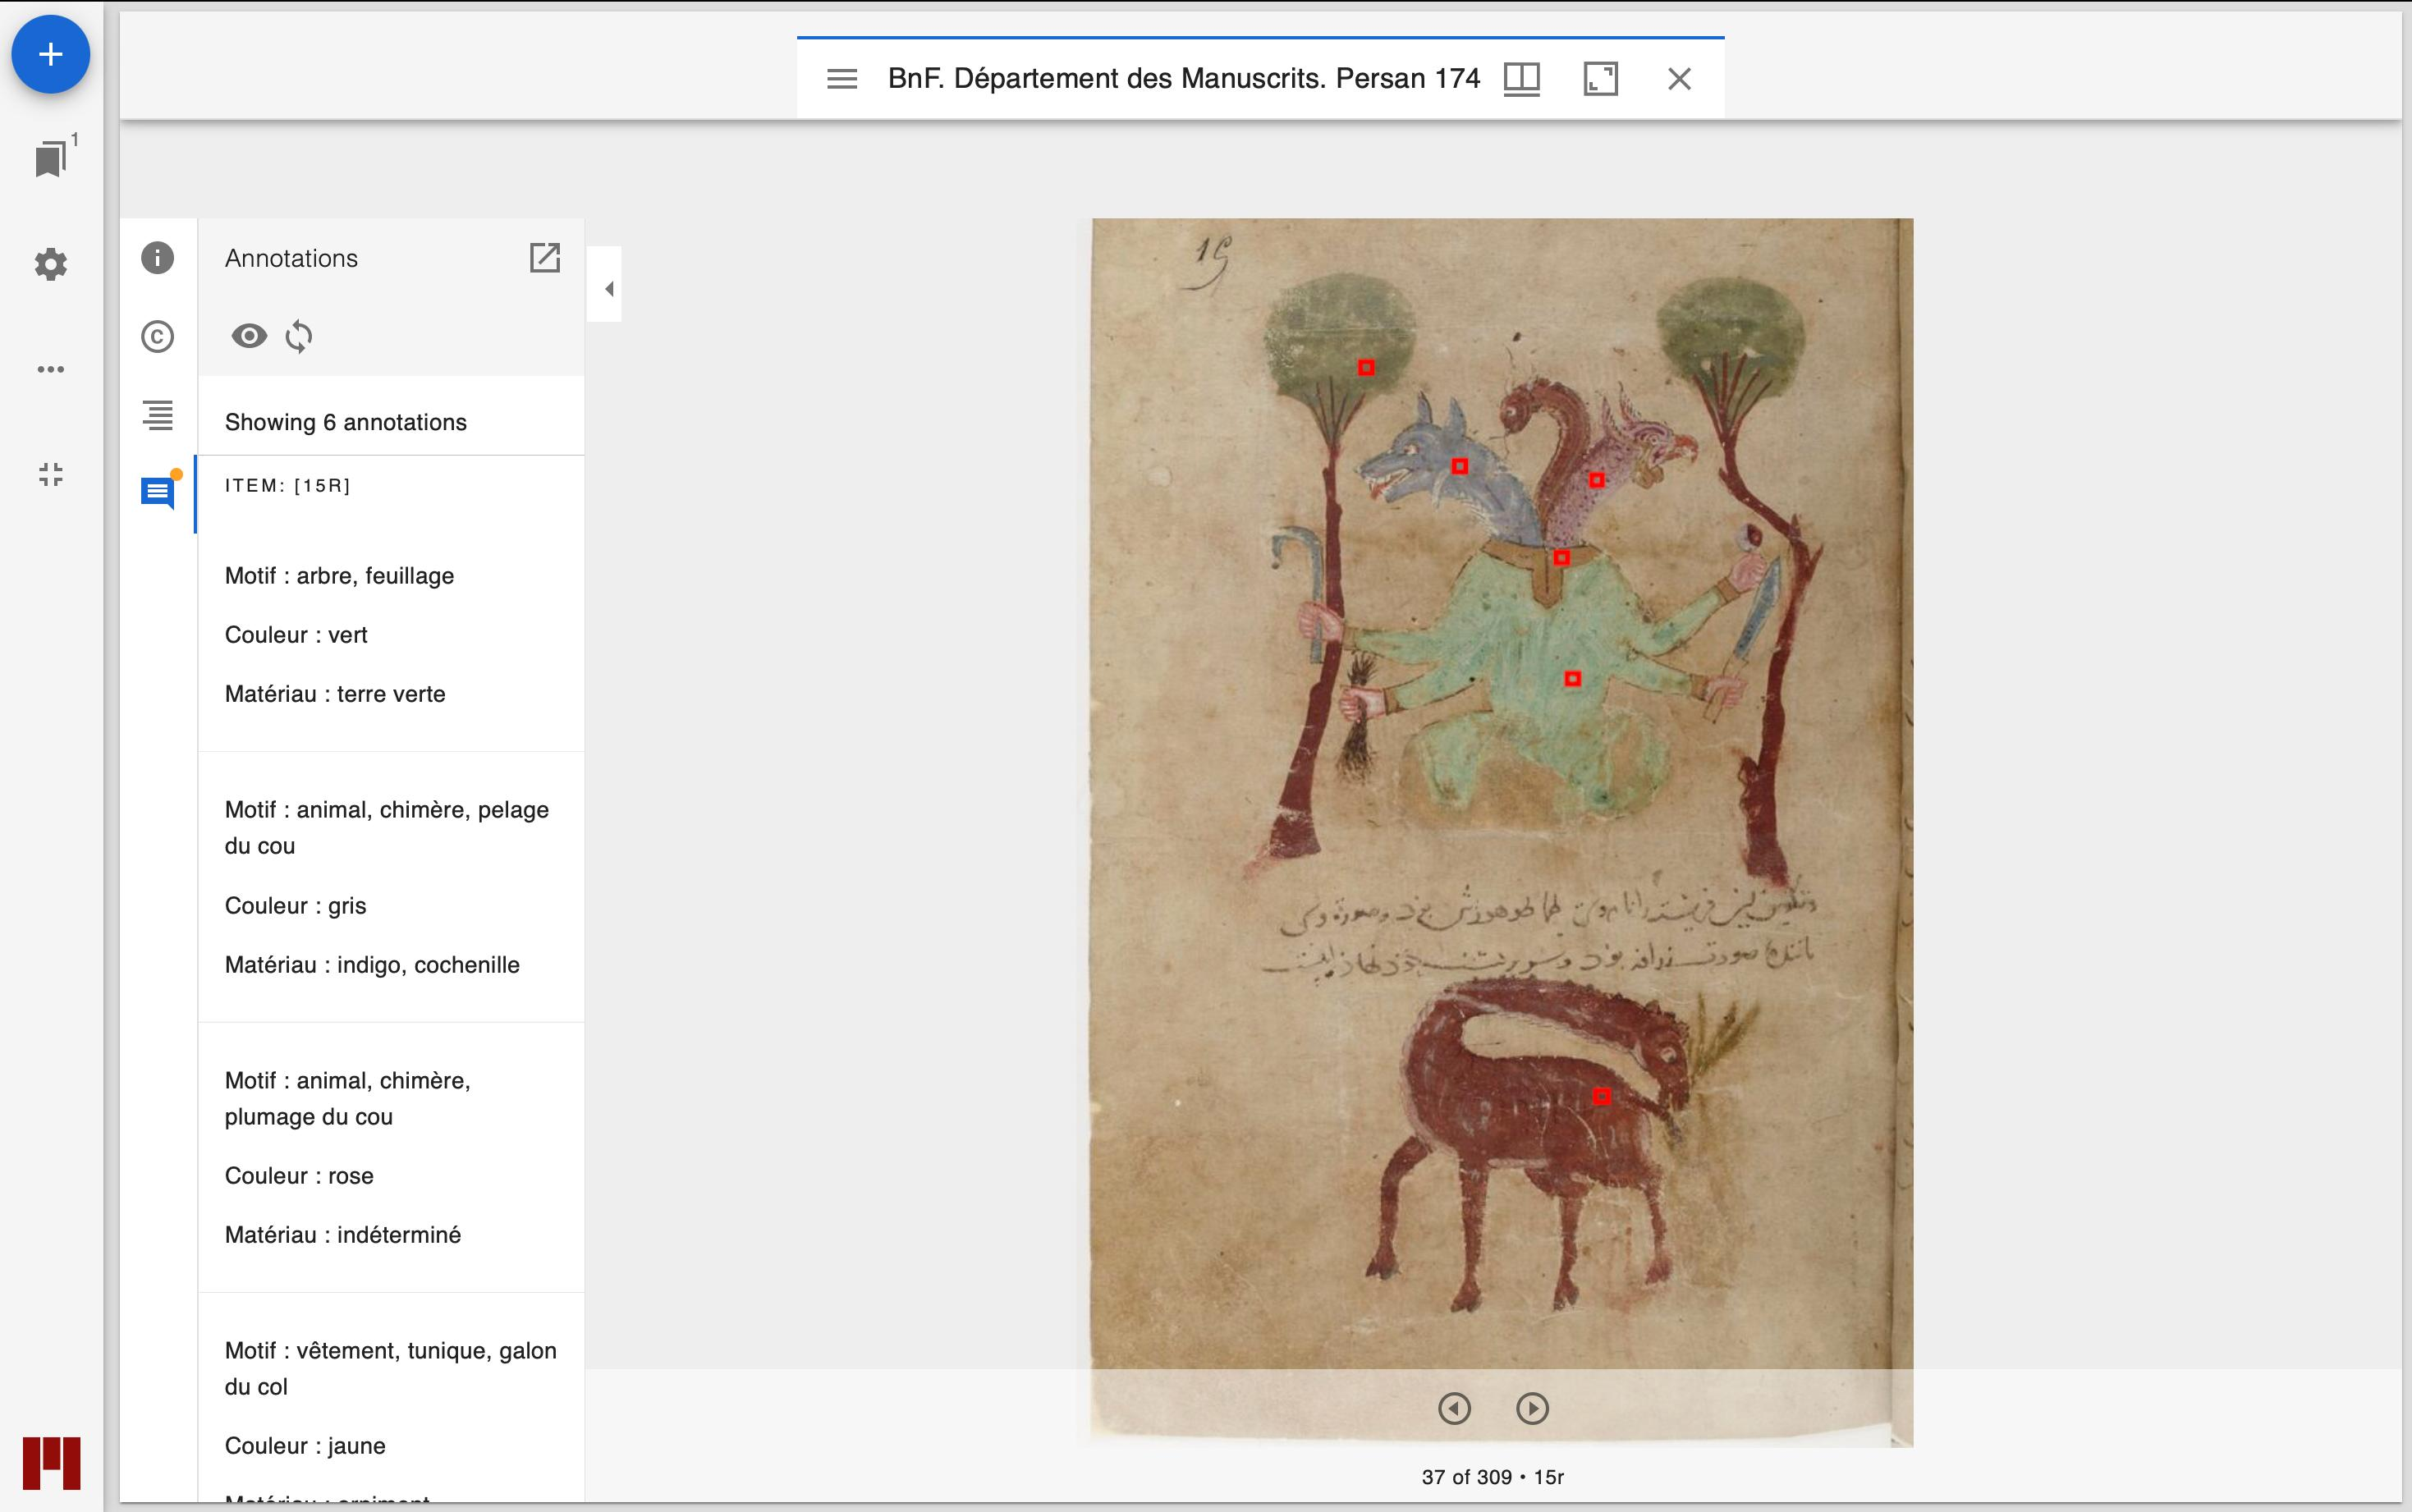
\includegraphics[width=\textwidth]{./textes/annexe/omeka-exemple.jpg}
	\label{fig:info}
\end{figure}
	\chapter[Retour critique]{Retour critique et problèmes techniques}
	\texttt{Leaflet}\par
La carte interactive proposée avec la bibliothèque JavaScript Leaflet fonctionne sans aucun défaut. Toutes ses fonctionnalités sont opérationnelles, qu'il s'agisse de l'affichage de la carte, des différents marqueurs et de leurs informations dans le carrousel et la barre latérale, ou de la combinaison des différents filtres. Cependant, je crois qu'une option supplémentaire aurait pu améliorer encore l'expérience de navigation et d'exploration des résultats. Actuellement, la carte interactive dévoile les résultats par feuillet, alors que les filtres portent sur les analyses. Ainsi, si le résultat d’un filtre ne correspond qu’à la troisième analyse d’un feuillet, il est nécessaire de faire défiler le carrousel jusqu’à l’apparition de la bonne analyse. Cet inconvénient ralentit quelque peu l’exploration de la carte, bien que les informations affichées demeurent correctes.\par
J'aurais souhaité, si la durée du stage me l’avait permis, de réaliser une seconde bascule dans les données, semblable à celle proposée pour le projet. Cette fois-ci, l’utilisateur aurait eu le choix de consulter les résultats par feuillet ou par manuscrit. Le carrousel aurait alors défilé les différentes pages analysées du manuscrit correspondant. Cette option aurait permis à l’utilisateur d’avoir une idée plus précise du nombre de manuscrits répondant à ses critères de sélection, ce qui est peut-être plus pertinent que d’obtenir le résultat par feuillet analysé.\\\par
\texttt{VIKUS Viewer}\par
La frise chronologique développée avec VIKUS Viewer présente un défaut majeur lors de son utilisation. Bien que l’articulation entre les différents paramètres fonctionne correctement et que les images apparaissent comme prévu lors de l'application des filtres, la cohérence de la barre latérale avec le feuillet affiché peut poser problème après un certain temps d’utilisation. Après une période indéterminée de navigation, les informations contenues dans la barre latérale se figent et ne correspondent plus à celles du feuillet sélectionné. Il est alors nécessaire de rafraîchir la visualisation. Ce dysfonctionnement est problématique pour les utilisateurs : non seulement ils doivent à nouveau renseigner leurs paramètres de recherche, mais ils doivent également faire preuve d'une grande vigilance pour éviter de recopier des informations erronées. J'ai inclus un avertissement dans le guide d’utilisation de la visionneuse à ce sujet. Cependant, ce défaut persiste et pose un réel problème. Il me semble qu'il pourrait être dû à la manière dont VIKUS déclare les variables et les met à jour. Malheureusement, dans le cadre de mon stage de trois mois, je n'ai pas eu l'occasion de pousser plus loin l’investigation ni de proposer une correction aux développeurs.\\\par
\texttt{Annotations IIIF}\par
Les annotations présentes dans les manifestes IIIF ne correspondent pas à celles initialement prévues. Le serveur d’annotations SAS permet de sélectionner un type de marqueur qui me semble bien plus précis que les carrés retenus et qui seront déployés sur le site Omeka~S. Après une phase de tests pour quelques annotations, j’ai constaté que les données~SVG (Scalable Vector Graphics) qui définissent ce marqueur étaient trop complexes pour la version de Mirador prévue pour Omeka~S. J’ai donc dû simplifier ces données et opter pour la représentation des analyses par petits carrés. De même, la version~3 de Mirador affiche le contenu des annotations dans une barre latérale, contrairement à la version précédente où elles apparaissaient dans une info-bulle. Cette modification rend l’information moins lisible.\par
De plus, l’implémentation de la visionneuse dans Omeka~S pose un problème quant à la gestion de certaines fonctionnalités de IIIF. Comme déjà souligné au cours de ce mémoire, il m’était impossible de proposer un affichage par calques, tel que je l’aurais souhaité initialement. Tous les calques se superposaient, et la seule solution a été d’abandonner cette possibilité. En revanche, la migration des données a été satisfaisante et toutes les informations qui devaient apparaître y figurent bien.
	\chapter[Liste des manifestes IIIF]{Liste des manifestes IIIF}
	Tous les manifestes IIIF et leurs annotations sont déposés sur le compte Github \url{https://workbench.gdmrdigital.com/login.xhtml}. Ils sont reliés à mon compte personnel, mais ils sont tous attribués à la Bibliothèque nationale de France. Ils peuvent être appelés par tout le monde à ces adresses~:\\\par
\texttt{Grec 139}~:\par
https://theoburnel.github.io/Grec139-v3/manifests/manifest\_3b.json\\\par
\texttt{NAL 1203}~:\par
https://theoburnel.github.io/NAL1203-v2/manifests/manifest2.json\\\par
\texttt{Latin 8878}~:\par
https://theoburnel.github.io/Latin8878-v2/manifests/manifest-3.json\\\par
\texttt{Latin 9389}~:\par
https://theoburnel.github.io/Latin9389-v4/manifests/manifest2.json\\\par
\texttt{Syriaque 341}~:\par
https://theoburnel.github.io/Syriaque341-v2/manifests/manifest2.json\\\par
\texttt{Copte 13}~:\par
https://theoburnel.github.io/Copte13-v2/manifests/manifest2.json\\\par
\texttt{Arabe 5847}~:\par
https://theoburnel.github.io/Arabe5847-v2/manifests/manifest2.json\\\par
\texttt{Mexicain 1-10}~:\par
https://theoburnel.github.io/Mexicain1-10/manifests/manifest.json\\\par
\texttt{Latin 10514}~:\par
https://theoburnel.github.io/Latin10514/manifests/manifest.json\\\par
\texttt{Supplément Grec 1296}~:\par
https://theoburnel.github.io/SupplementGrec-1286/manifests/manifest.json\\\par
\texttt{Latin 10525}~:\par
https://theoburnel.github.io/Latin10525/manifests/manifest.json\\\par
\texttt{Persan 174}~:\par
https://theoburnel.github.io/Persan174/manifests/manifest.json
	\chapter[Liens des projets]{Liens vers la carte interactive et la frise chronologique}
	\begin{itemize}
	\item Lien vers la carte Leaflet~:\par \url{https://github.com/TheoBurnel/Stage.git}\\
	\item Lien vers la frise VIKUS~:\par \url{https://github.com/TheoBurnel/vikus_bnf.git}
\end{itemize}

	\newpage{\pagestyle{empty}\cleardoublepage}
	
	%%%%%%%%%%%%%%%%%%
	\backmatter
	
	\printindex
	\listoffigures
	\tableofcontents
\end{document}